\documentclass[a4paper]{article}
\usepackage[T1]{fontenc}			% pacchetto per \chapter
\usepackage[italian]{babel}
\usepackage[italian]{isodate}  		% formato delle date in italiano
\usepackage{lipsum}
\usepackage{graphicx}				% gestione delle immagini
\usepackage{amsfonts}
\usepackage{booktabs}				% tabelle di qualità superiore
\usepackage{amsmath}				% pacchetto matematica
\usepackage{amsthm}					% teoremi migliorati
\usepackage{enumitem}				% gestione delle liste
\usepackage{pifont}					% pacchetto con elenchi carini
\usepackage{listings}				% pacchetto per i codici
\usepackage{caption}
\usepackage{cancel}
\usepackage[x11names]{xcolor}		% pacchetto colori RGB
% Link ipertestuali per l'indice
\usepackage{xcolor}
\usepackage[linkcolor=black, citecolor=blue, urlcolor=cyan]{hyperref}
\hypersetup{
	colorlinks=true
}

\definecolor{codegreen}{rgb}{0,0.6,0}
\definecolor{codegray}{rgb}{0.5,0.5,0.5}
\definecolor{codepurple}{rgb}{0.58,0,0.82}
\definecolor{backcolour}{rgb}{0.95,0.95,0.92}
\lstdefinestyle{mystyle}{
	backgroundcolor=\color{backcolour},   
	commentstyle=\color{codegreen},
	keywordstyle=\color{magenta},
	numberstyle=\tiny\color{codegray},
	stringstyle=\color{codepurple},
	basicstyle=\ttfamily\footnotesize,
	breakatwhitespace=false,         
	breaklines=true,                 
	captionpos=b,                    
	keepspaces=true,                 
	numbers=left,                    
	numbersep=5pt,                  
	showspaces=false,                
	showstringspaces=false,
	showtabs=false,                  
	tabsize=2
}
\lstset{style=mystyle}

\definecolor{maroon}{rgb}{0.5,0,0}
\definecolor{darkgreen}{rgb}{0,0.5,0}
\lstdefinelanguage{XML}
{
	basicstyle=\ttfamily\footnotesize,
	morestring=[s]{"}{"},
	morecomment=[s]{?}{?},
	morecomment=[s]{!--}{--},
	commentstyle=\color{darkgreen},
	moredelim=[s][\color{black}]{>}{<},
	moredelim=[s][\color{red}]{\ }{=},
	stringstyle=\color{blue},
	identifierstyle=\color{maroon}
}

%\usepackage{showframe}				% visualizzazione bordi
%\usepackage{showkeys}				% visualizzazione etichetta

\newcommand{\longline}{\noindent\rule{\textwidth}{0.4pt}}
\newcommand{\dquotes}[1]{``#1''}
\renewcommand{\qedsymbol}{QED}

\begin{document}
	\author{VR443470}
	\title{Esami - Basi di dati}
	\date{\printdayoff\today}
	\maketitle

	\newpage
	
	% indice
	\tableofcontents
	
	\newpage
		
	\section{Domande di teoria - Primo parziale}
	
	Le domande più frequenti che si possono incontrare nel primo parziale di Basi di dati sono:
	\begin{enumerate}
		\item Si illustri il concetto/costrutto di \textbf{entità} nel modello Entità-Relazione.
		
		\item Si illustri il concetto/costrutto di \textbf{relazione} nel modello Entità-Relazione.
		
		\item Si illustri il concetto/costrutto di \textbf{generalizzazione} nel modello Entità-Relazione.
		
		\item Si illustri il concetto/costrutto di \textbf{identificatore} nel modello Entità-Relazione.
		
		\item Si illustri il concetto/costrutto di \textbf{superchiave} nel modello Entità-Relazione.
		
		\item Si illustri il concetto/costrutto di \textbf{attributo multivalore} nel modello Entità-Relazione.
	\end{enumerate}
	La risposta, per essere considerata perfetta, deve includere le seguenti caratteristiche:
	\begin{itemize}
		\item Semantica
		\item Sintassi grafica con esempio
		\item Istanza
		\item Eventuali proprietà
	\end{itemize}
	Qui di seguito vengono date le possibili risposte alle domande di teoria:
	\begin{enumerate}
		\item \textcolor{Green4}{\emph{Si illustri il concetto/costrutto di \textbf{entità} nel modello Entità-Relazione.}}
		
		\textbf{Semantica}. L'entità rappresenta una classe di oggetti che hanno proprietà comuni ed esistenza \dquotes{autonoma} ai fini dell'applicazione di interesse. Il nome dato ad ogni entità è identificativo di quella determinata classe di oggetti e deve essere univoco all'interno dello schema.\newline
		\textbf{Sintassi grafica}. Per esempio, l'entità studenti rappresenta la classe di oggetti degli studenti di un'università e gli attributi possibili possono essere: matricola, nome, cognome, data di nascita, ecc. La sintassi grafica è la seguente:
		\begin{figure}[!htp]
			\centering
			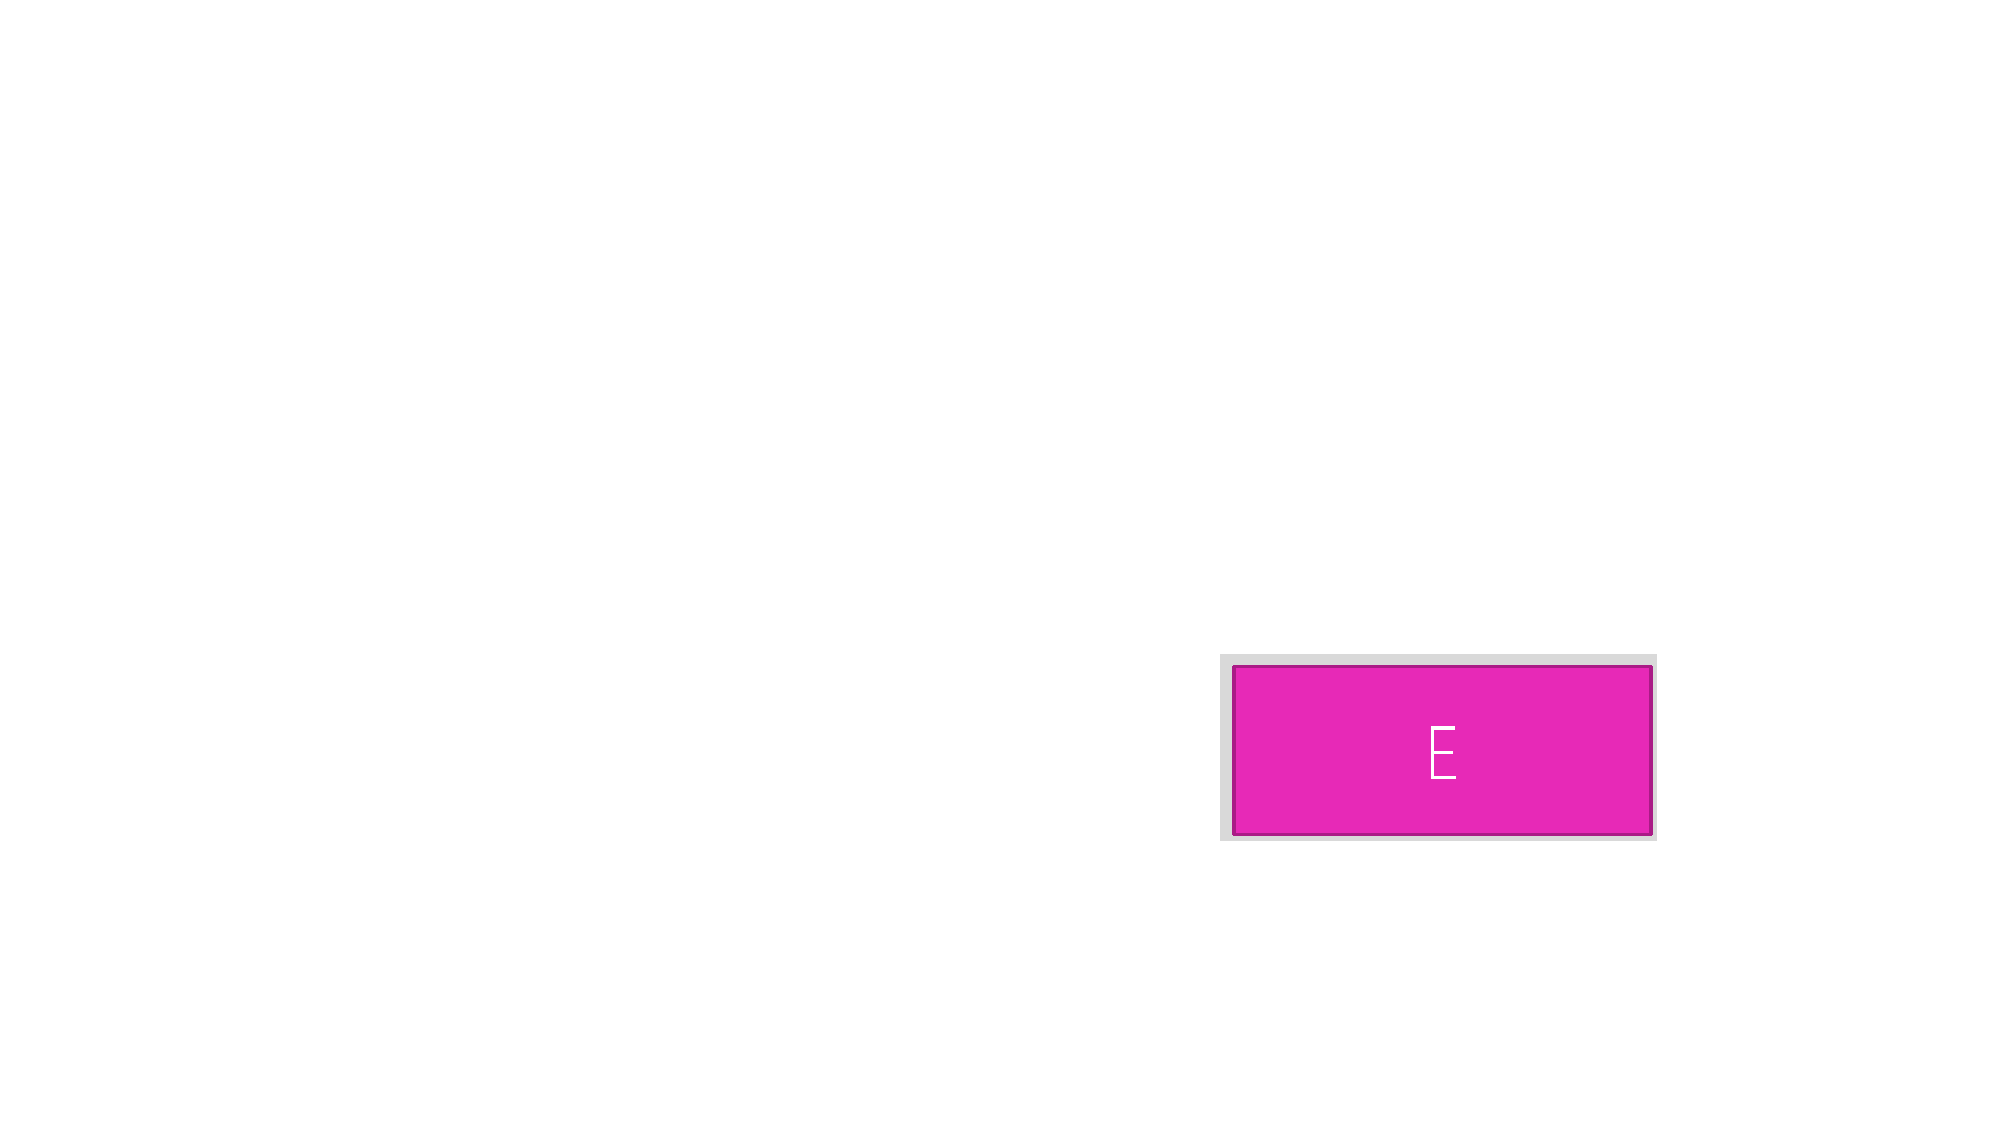
\includegraphics[width=.3\textwidth]{img/entita_def.pdf}
		\end{figure}
		
		\noindent
		\textbf{Istanza}. L'istanza di un'entità è un oggetto della classe che lo rappresenta e non un unico valore. Per esempio, nell'entità studenti, lo studente Mario Rossi (in carne ed ossa) rappresenta un'istanza dell'entità.
		\newpage
		
		
		\item \textcolor{Green4}{\emph{Si illustri il concetto/costrutto di \textbf{relazione} nel modello Entità-Relazione.}}
		
		\textbf{Semantica}. La relazione rappresenta legami logici tra una o più entità. Ogni relazione deve avere un nome univoco all'interno dello schema e non può avere identificatori. Esistono due tipi di relazioni: \emph{ricorsive}, cioè in cui è coinvolta una sola entità, \emph{n-arie}, in cui sono coinvolte \emph{n} entità. Esse nascono solo quando le entità coinvolte contengono almeno una tupla.\newline
		\textbf{Sintassi grafica}. Un esempio di relazione è la \dquotes{Residenza} tra le entità \dquotes{Città} e \dquotes{Impiegato}. La sua sintassi grafica è un rombo:
		\begin{figure}[!htp]
			\centering
			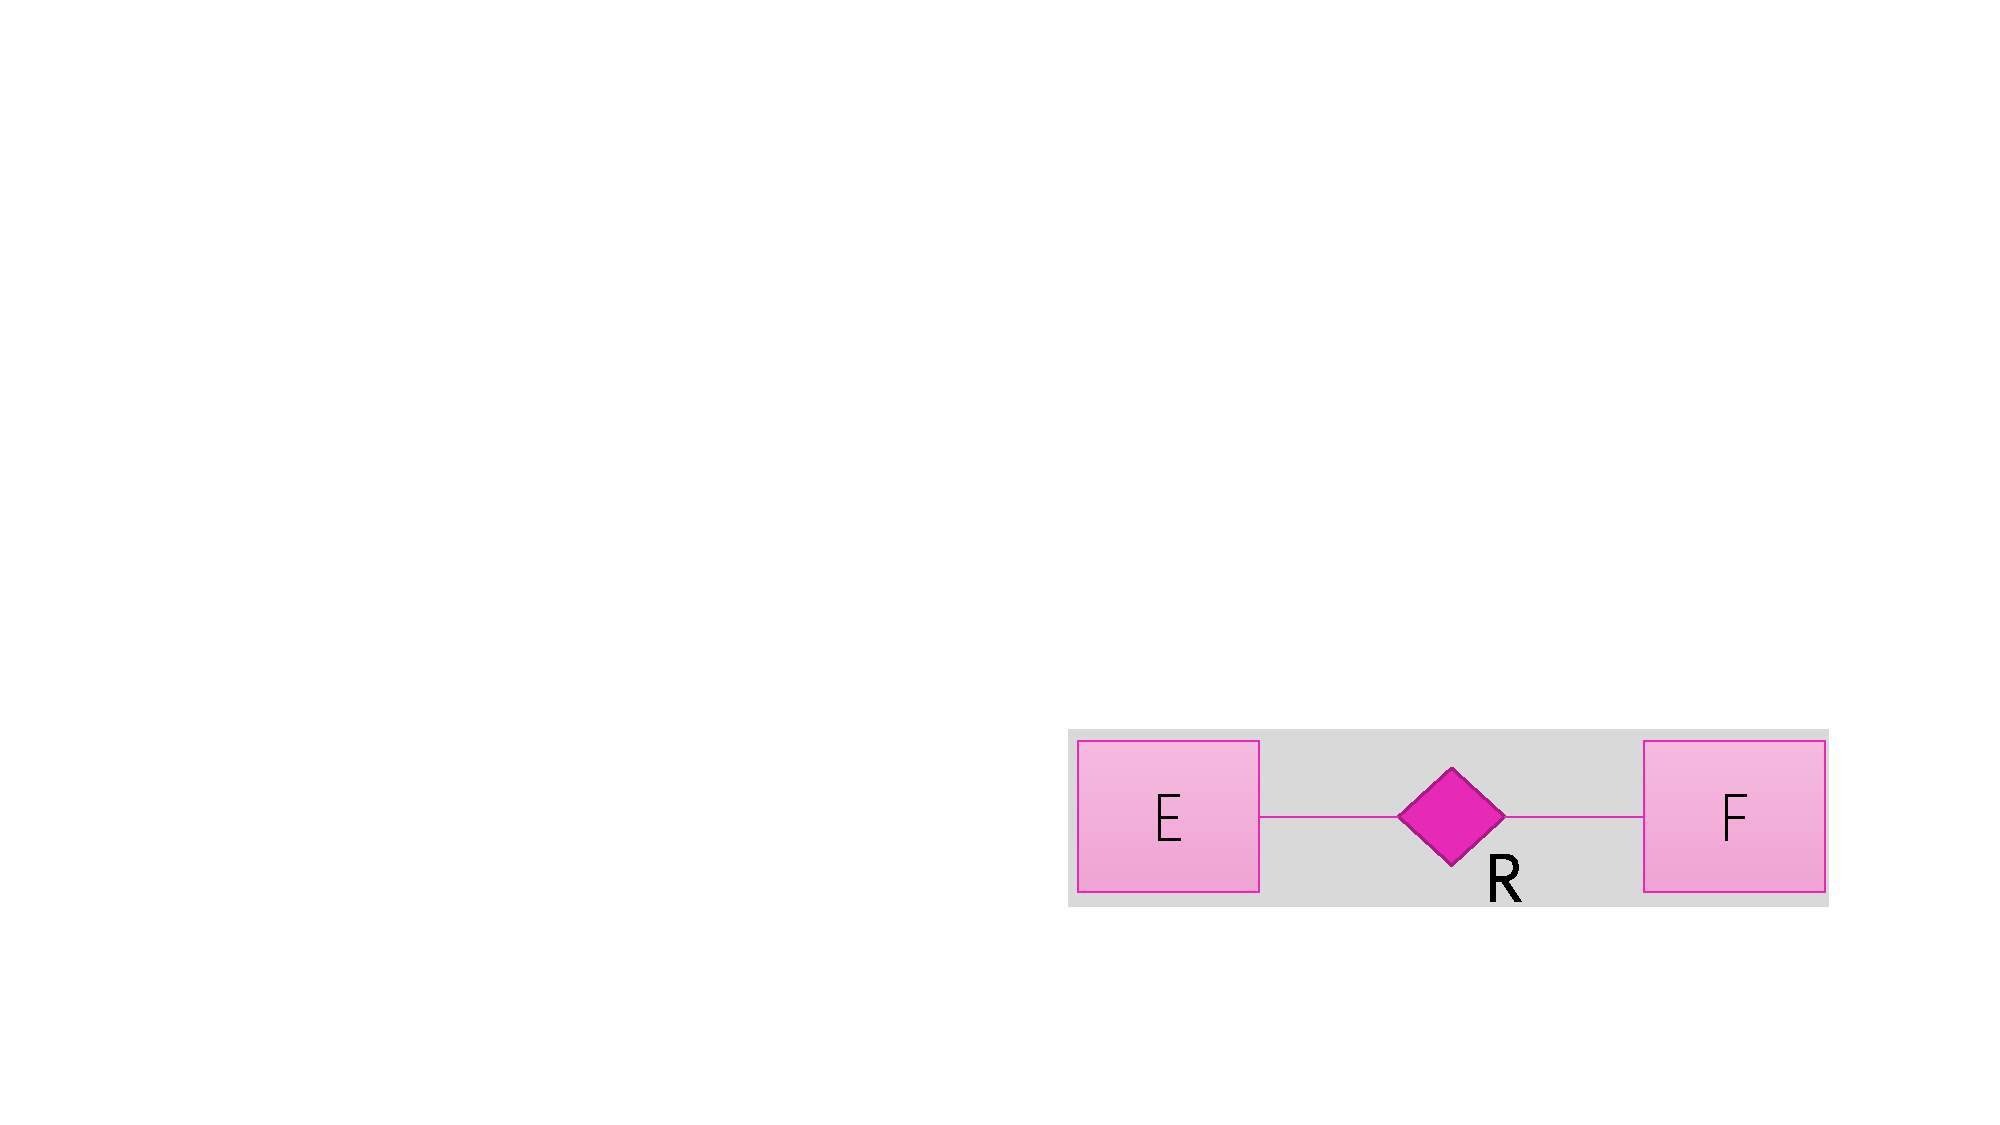
\includegraphics[width=.5\textwidth]{img/relazione_def.pdf}
		\end{figure}
		
		\noindent
		\textbf{Istanza}. Data una relazione $R$ tra $n$ entità $E_{1}, E_{2}, ..., E_{n}$, un'istanza è composta da una ennupla del tipo:
		\begin{equation*}
			\left(e_{1}, e_{2}, ..., e_{i}\right) \: \text{dove} \: e_{i} \in I\left(E_{i}\right), 1 \le i \le n
		\end{equation*}
		Inoltre, esiste un'importante proprietà che afferma:
		\begin{equation*}
			I\left(R\right) \subseteq I\left(E_{1}\right) \times I\left(E_{2}\right) \times ... \times I\left(E_{n}\right)
		\end{equation*}
		\newpage
		
		
		\item \textcolor{Green4}{\emph{Si illustri il concetto/costrutto di \textbf{generalizzazione} nel modello Entità-Relazione.}}
		
		\textbf{Semantica}. Le generalizzazioni rappresentano legami logici tra un'entità $E$, chiamata genitore, e più entità $E_{1}, ..., E_{n}$, chiamate figlie. Quindi, si dice che l'entità $E$ (genitore) è la generalizzazione delle entità $E_{1},...,E_{n}$ (figlie) e quest'ultime vengono chiamate specializzazioni. Inoltre, ogni occorrenza dell'entità figlia è anche un'occorrenza dell'entità padre, e ogni proprietà dell'entità padre è anche una proprietà dell'entità figlia.\newline
		La classificazioni sono coppie di valori che hanno diverso significato:
		\begin{itemize}
			\item (totale, esclusiva)
			
			\item (totale, sovrapposta)
			
			\item (parziale, esclusiva)
			
			\item (parziale, sovrapposta)
		\end{itemize}
		Con totale, il genitore ha ogni occorrenza posseduta da almeno un'entità figlia. In caso contrario è parziale.\newline
		Con esclusiva, il genitore ha ogni occorrenza che si ripete solamente in una delle entità figlie. In caso un'occorrenza del genitore sia di più entità figlie, si dice sovrapposta.\newline
		\textbf{Sintassi grafica}. Un esempio è la generalizzazione \dquotes{Persona} con le specializzazioni \dquotes{Uomo} e \dquotes{Donna}. La sintassi grafica:
		\begin{figure}[!htp]
			\centering
			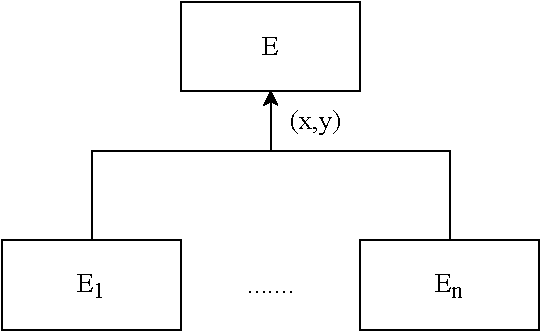
\includegraphics[width=.5\textwidth]{img/generalizzazione_sintassi.pdf}
		\end{figure}
		\newpage
		
		
		\item \textcolor{Green4}{\emph{Si illustri il concetto/costrutto di \textbf{identificatore} nel modello Entità-Relazione.}}
		
		\textbf{Semantica}. Gli identificatori descrivono i concetti (attributi/entità) dello schema che consentono di identificare in maniera univoca le occorrenze delle entità. Devono essere specificati per ogni entità e non possono apparire all'interno di relazioni. Un identificatore può essere:
		\begin{itemize}
			\item Interno, ovvero viene scelto un attributo dell'entità;
			\item Esterno, viene scelto un identificatore di un'altra identità;
		\end{itemize}
		È possibile utilizzare sia identificatori interni ed esterni insieme.\newline
		\textbf{Sintassi grafica}. Un esempio è l'entità \dquotes{Studente} che possiede come identificatore la \dquotes{Matricola} poiché unica. La sintassi grafica:
		\begin{figure}[!htp]
			\centering
			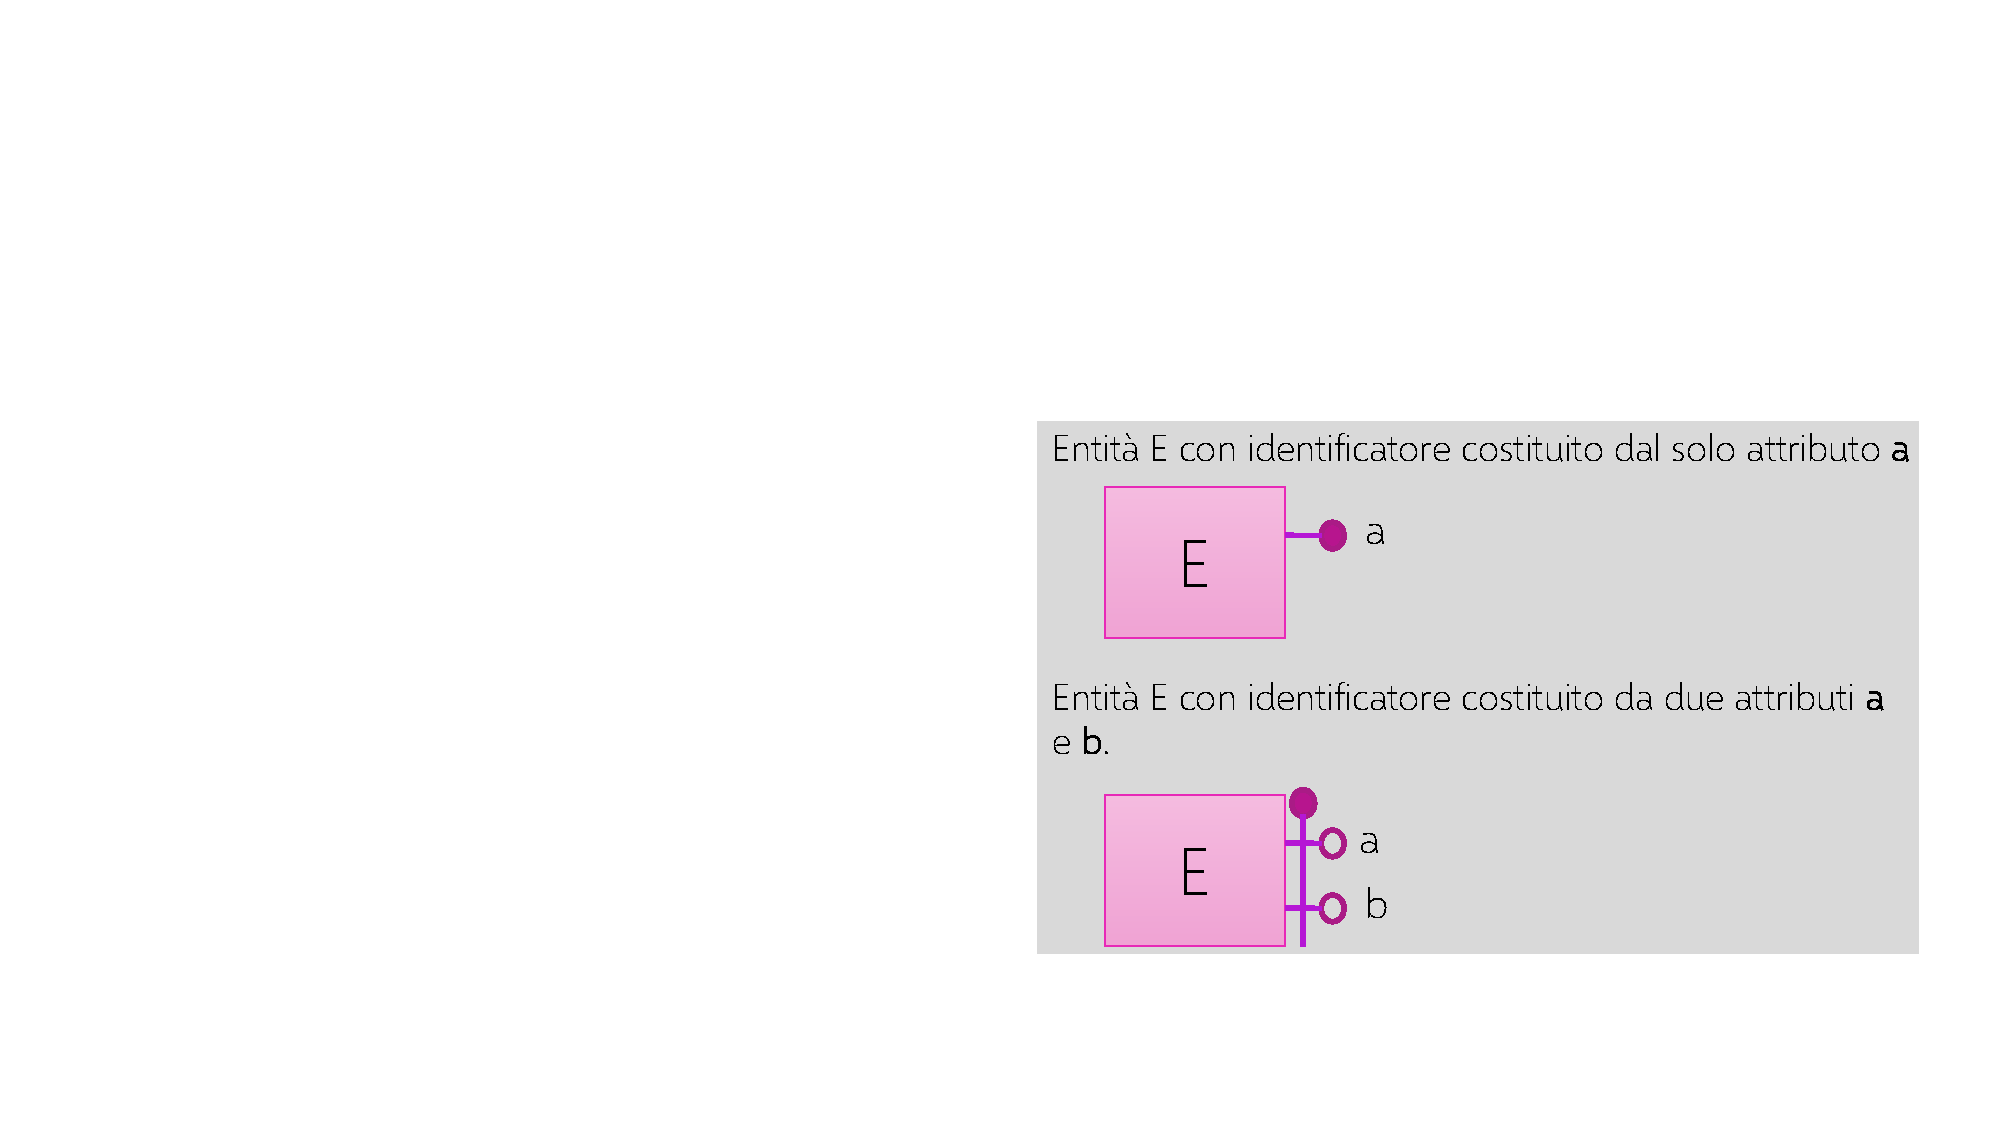
\includegraphics[width=.6\textwidth]{img/identificatore_def.pdf}
		\end{figure}
		
		
		\item \textcolor{Green4}{\emph{Si illustri il concetto/costrutto di \textbf{superchiave} nel modello Entità-Relazione.}}
		
		\textbf{Semantica}. Una superchiave è un'insieme di attributi che non contiene tuple duplicate al suo interno. Una superchiave è una chiave prima se e solo se è una superchiave minimale. Invece, una chiave primaria è sempre superchiave (non viceversa!).\newline
		\textbf{Sintassi grafica}. Non esiste una sintassi grafica poiché è un concetto, ma un esempio:
		\begin{figure}[!htp]
			\centering
			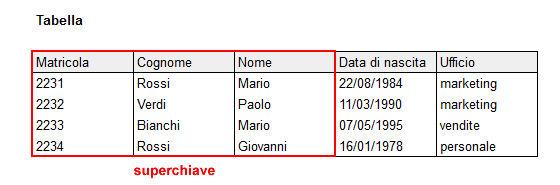
\includegraphics[width=\textwidth]{img/superchiave.png}
		\end{figure}
		
		\noindent
		Nessuna tupla si ripete, quindi \dquotes{Matricola, Cognome, Nome} è una superchiave valida. Non è minimale poiché esiste \dquotes{Matricola} che è chiave primaria e superchiave minimale.
		\newpage
		
		
		\item \textcolor{Green4}{\emph{Si illustri il concetto/costrutto di \textbf{attributo} nel modello Entità-Relazione.}}
		
		\textbf{Semantica}. Gli attributi descrivono le proprietà elementari di entità o relazioni che sono di interesse ai fini dell'applicazione. Ogni attributo ha un suo dominio e quindi può essere visto come una funzione che ha come dominio le istanze dell'entità/relazione e come codominio l'insieme dei valori ammissibili:
		\begin{equation*}
			f_{a} : I\left(E\right) \rightarrow D
		\end{equation*}
		Dove $a$ è un attributo dell'entità $E$, $I\left(E\right)$ è l'insieme delle istanze di $E$ e $D$ è l'insieme dei valori ammissibili.\newline
		\textbf{Sintassi grafica}. Un esempio di attributo è \dquotes{Cognome}, \dquotes{Stipendio} ed \dquotes{Età} dell'entità \dquotes{Impiegato}. La sintassi grafica è la seguente:
		\begin{figure}[!htp]
			\centering
			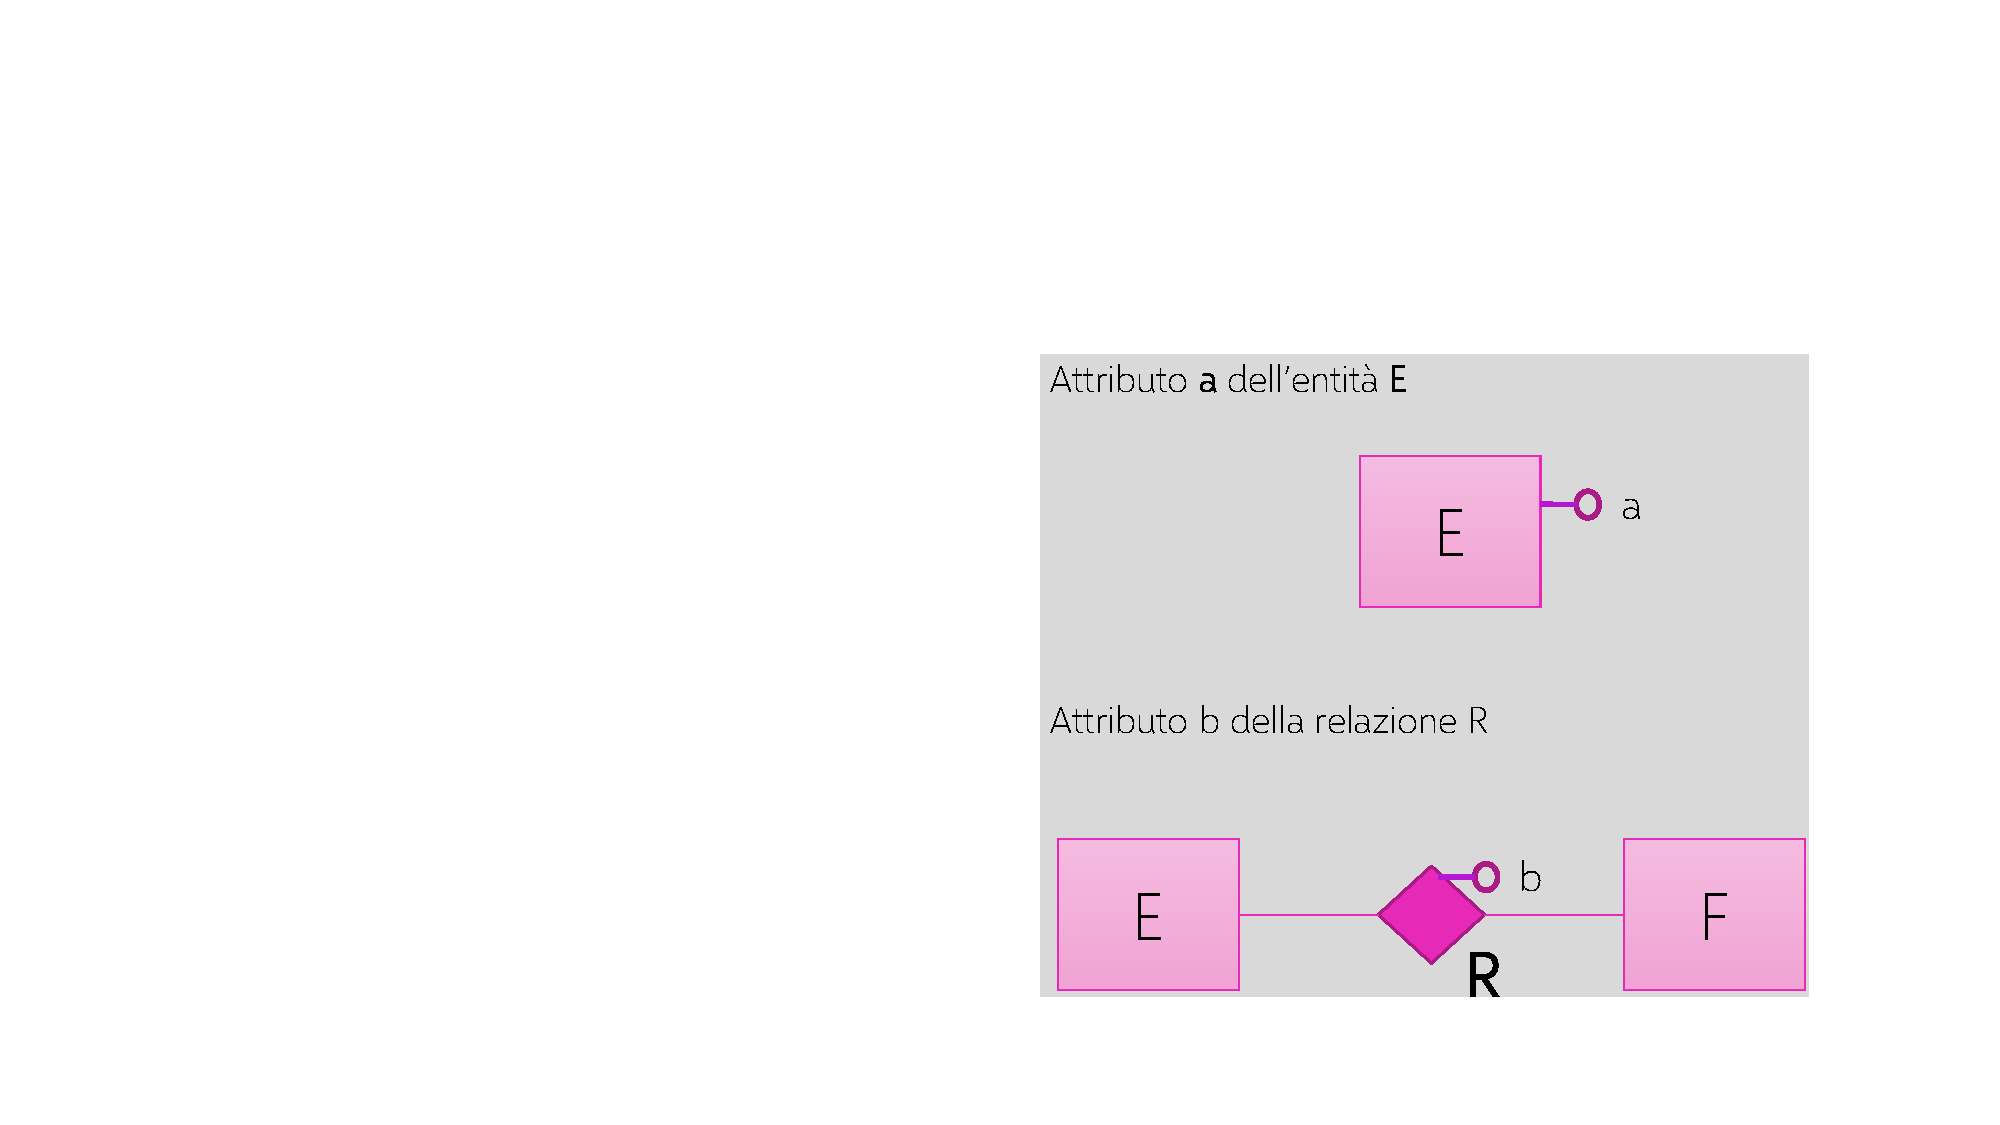
\includegraphics[width=.5\textwidth]{img/attributo_def.pdf}
		\end{figure}
		
		\noindent
		\textbf{Istanza}. L'istanza si ottiene tramite una funzione che data un'istanza dell'entità $E$ (o relazione $R$), restituisce l'attributo $a$:
		\begin{equation*}
			\text{valore di} \: a \: \text{su} \: e = f_{a}\left(e\right)
		\end{equation*}
	\end{enumerate}\newpage
	
	\section{Esercizi terzo parziale}
	
	\subsection[$\mathrm{B^{+}\text{-}tree}$]{$\boldsymbol{\mathrm{B^{+}\text{-}tree}}$}
	
	\subsubsection{Esercizio 1}
	
	Costruire un $\mathrm{B}^{+}$-tree di $\text{fan-out} = 5$ con i seguenti nodi foglia: $\left(A,B,C,D\right)$, $\left(F,G,M,N\right)$, $\left(O,P\right)$, $\left(S,T\right)$, $\left(W,Z\right)$. I vincoli di riempimento sono:
	\begin{itemize}
		\item $2 \le \text{\#chiavi} \le 4$
		
		\item $3 \le \text{\#puntatori} \le 5$
	\end{itemize}
	Dopodiché, inserire il valore chiave H nel $\mathrm{B}^{+}$-tree ottenuto precedentemente. Infine, l'esercizio si conclude eseguendo una rimozione del valore chiave Z ottenuto precedentemente.\newline
	
	\noindent
	\textcolor{Green4}{\textbf{\emph{\underline{Soluzione}}}}\newline
	
	\noindent
	Il primo passo è costruire i vari livelli dei nodi foglia:
	\begin{figure}[!htp]
		\centering
		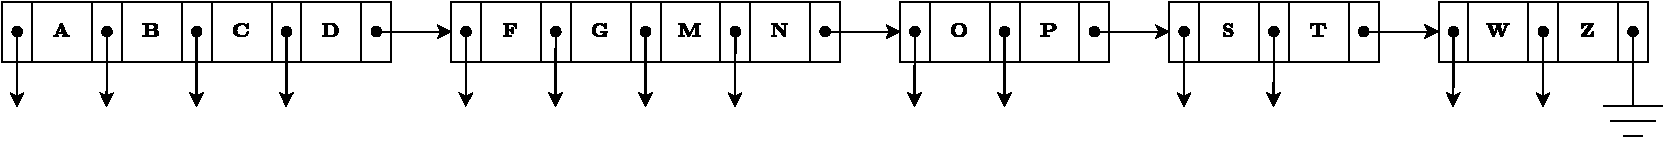
\includegraphics[width=\textwidth]{img/b+-tree.pdf}
	\end{figure}
	
	\noindent
	Adesso è necessario costruire tutti i puntatori richiesti. Fan-out è uguale a 5 quindi viene costruito un nodo intermedio con 5 puntatori e si collegano tutti i nodi:
	\begin{figure}[!htp]
		\centering
		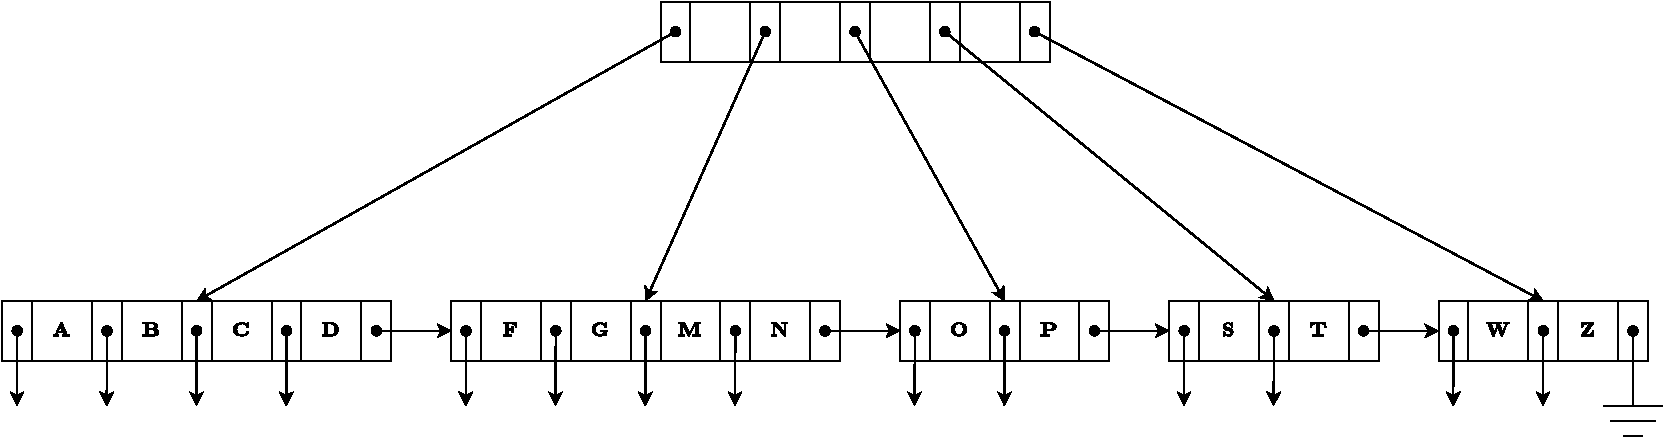
\includegraphics[width=\textwidth]{img/b+-tree-1.pdf}
	\end{figure}
	
	\noindent
	Adesso si aggiungono le lettere che devono essere raggiunte dopo aver visitato ogni nodo:
	\begin{figure}[!htp]
		\centering
		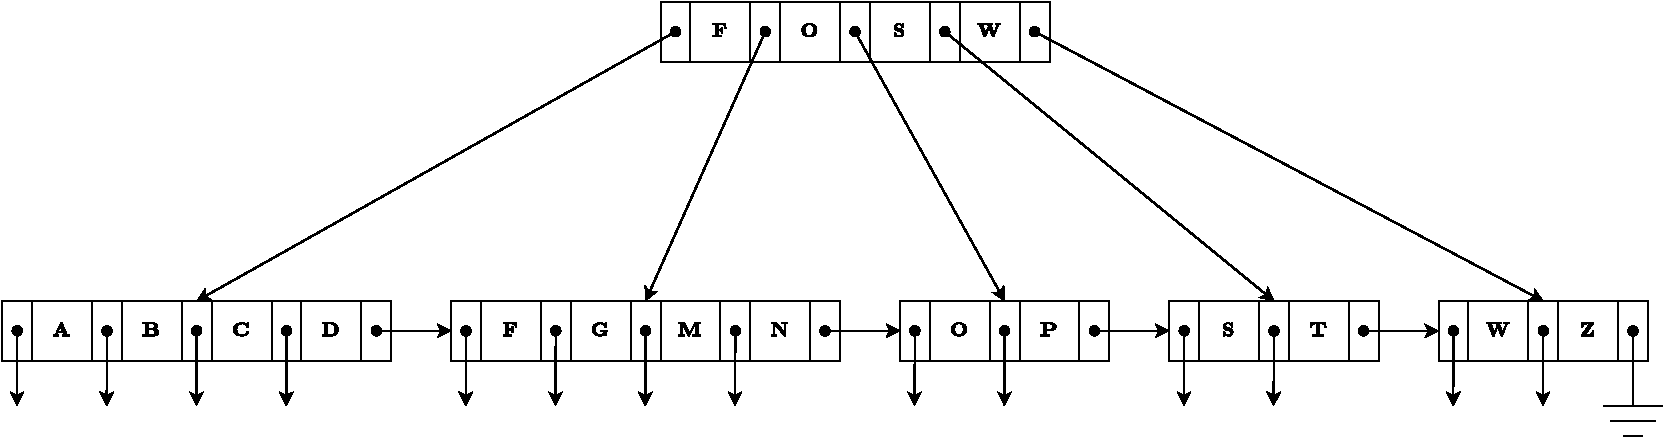
\includegraphics[width=\textwidth]{img/b+-tree-2.pdf}
	\end{figure}\newpage
	
	\noindent
	Per inserire il valore chiave è necessario avere a disposizione una posizione libera. Tuttavia, questo non è possibile, per cui viene applicato uno split. Viene divisa la radice contenente $\left(F,G,M,N\right)$ così da inserire la chiave H tra la G e la M:
	\begin{figure}[!htp]
		\centering
		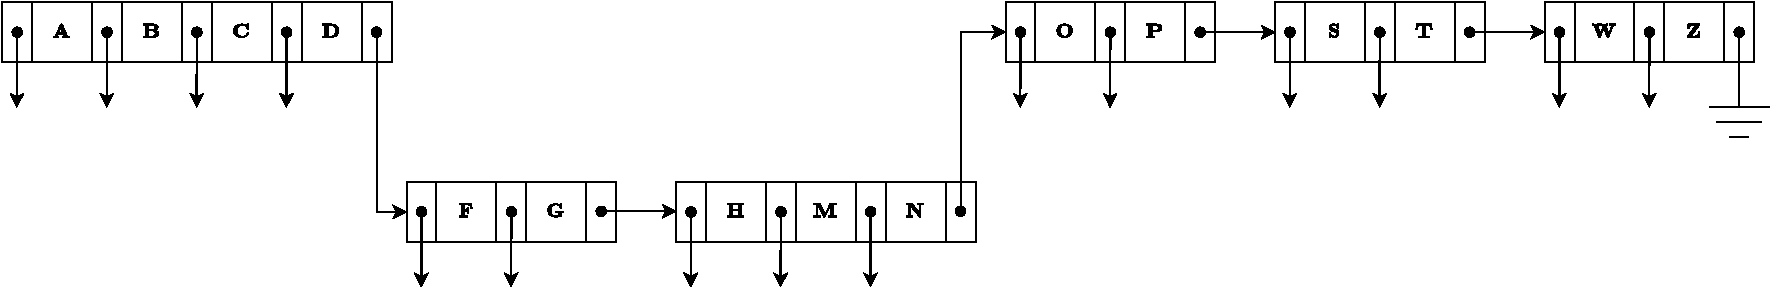
\includegraphics[width=\textwidth]{img/b+-tree-3.pdf}
	\end{figure}
	
	\noindent
	A questo punto è necessario riadattare il nodo radice che attualmente punta ad un nodo errato (attenzione c'è un errore, il nodo V in realtà è il nodo W):
	\begin{figure}[!htp]
		\centering
		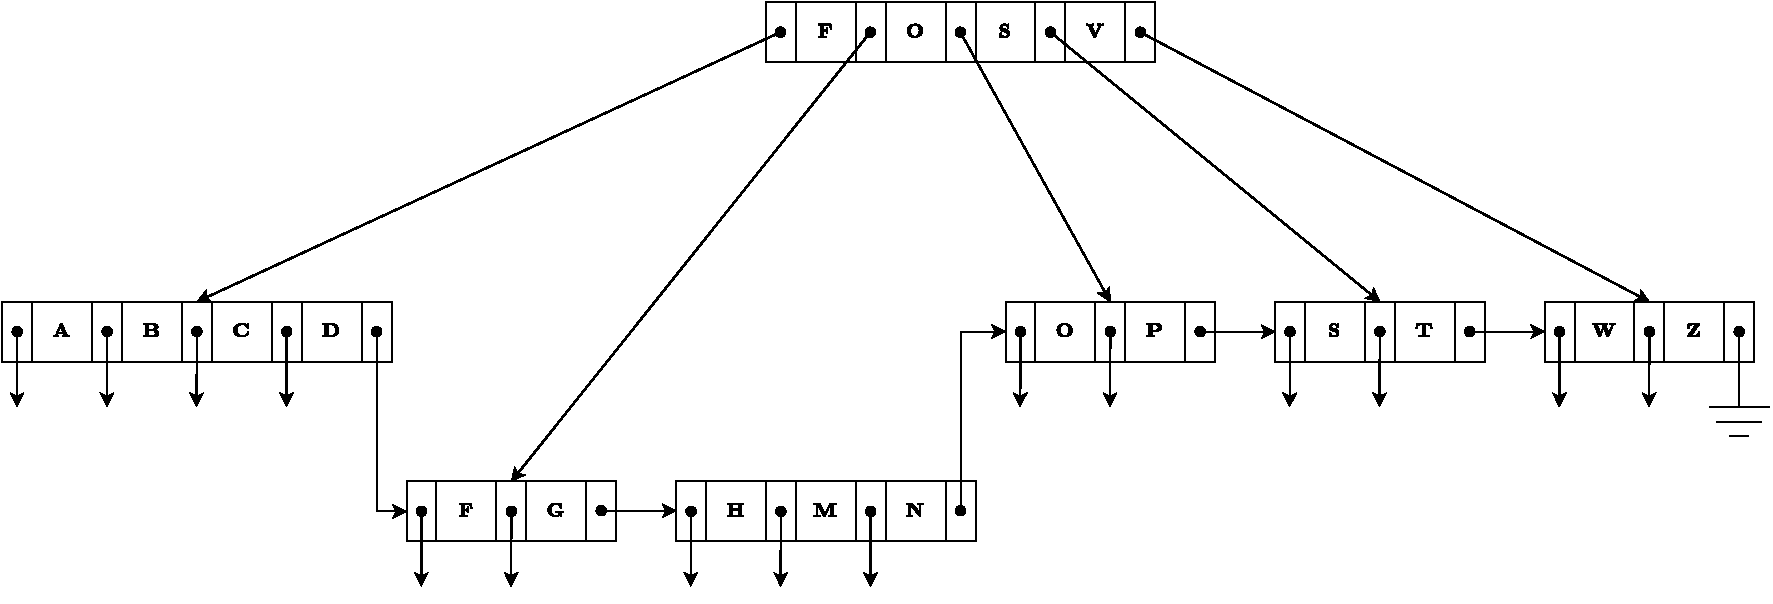
\includegraphics[width=\textwidth]{img/b+-tree-4.pdf}
	\end{figure}
	
	\noindent
	Per farlo, è necessario eseguire una divisione anche nel nodo radice aggiustando i valori delle chiavi (attenzione c'è un errore, il nodo V in realtà è il nodo W):
	\begin{figure}[!htp]
		\centering
		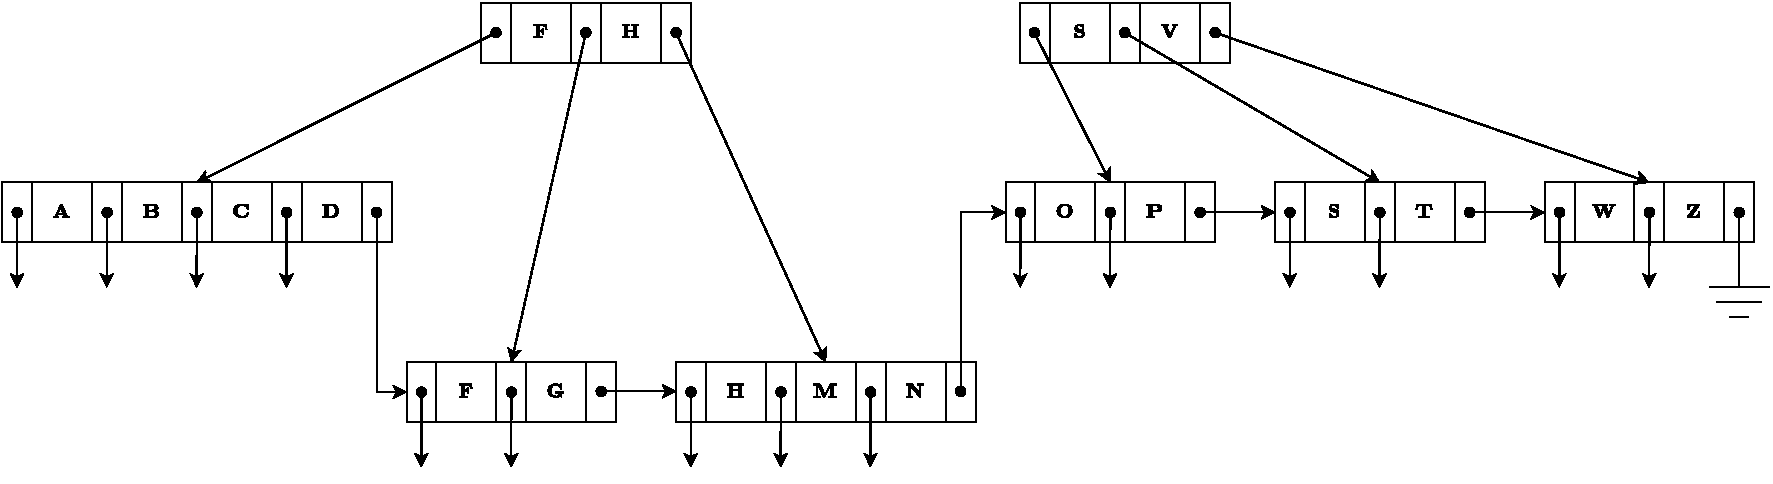
\includegraphics[width=\textwidth]{img/b+-tree-5.pdf}
	\end{figure}\newpage
	
	\noindent
	E infine, collegare i due nodi divisi con un nodo di congiunzione. Inoltre, quest'ultimo viene riempito con un valore chiave (attenzione c'è un errore, il nodo V in realtà è il nodo W):
	\begin{figure}[!htp]
		\centering
		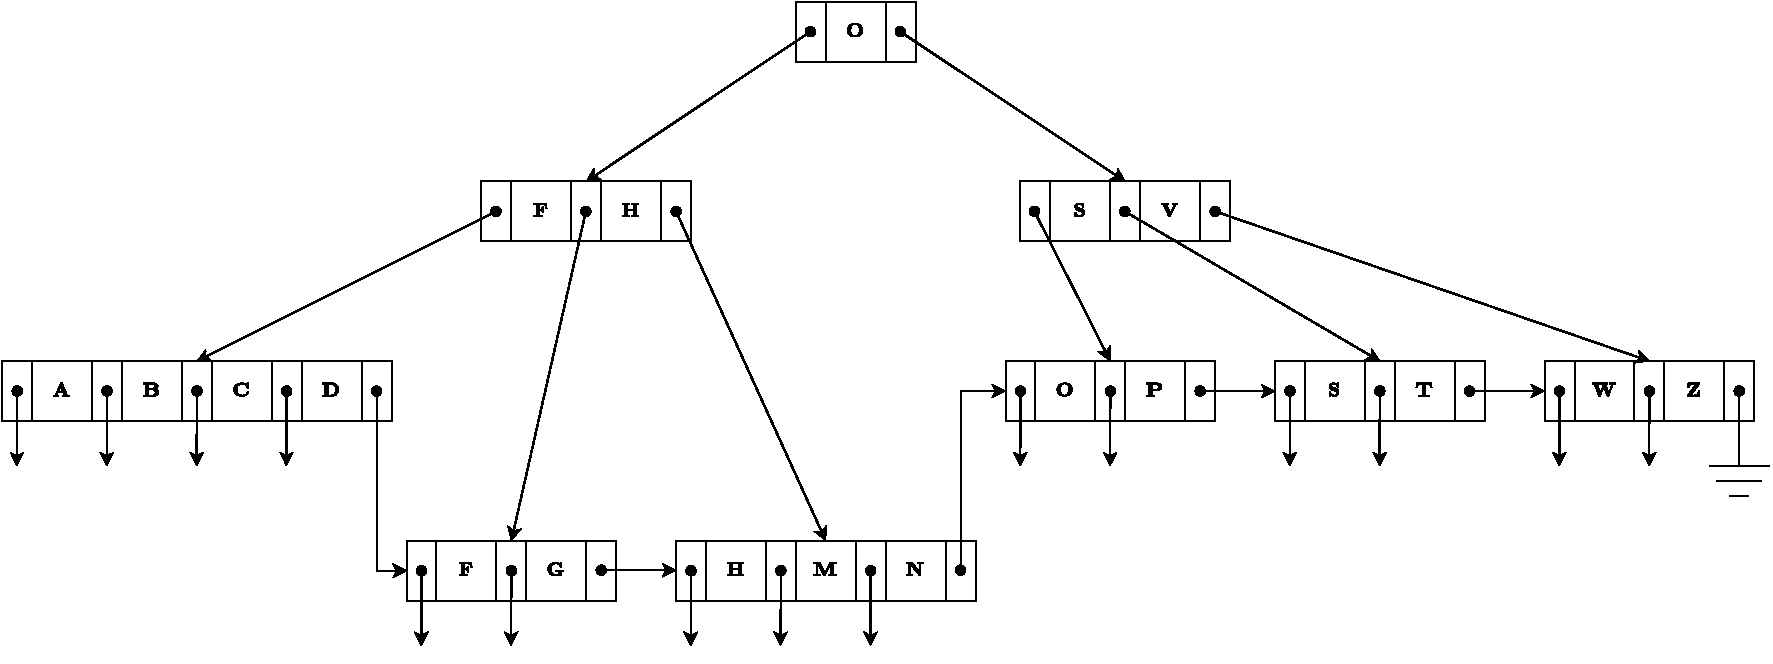
\includegraphics[width=\textwidth]{img/b+-tree-6.pdf}
	\end{figure}
	
	\noindent
	La rimozione della chiave Z comporta che l'ultimo nodo abbia come chiave solo il valore W. Questo comporta un'irregolarità poiché il numero minimo di ogni chiave in ogni nodo deve essere minimo di due e massimo di quattro. Per cui è necessario effettuare un merge:
	\begin{figure}[!htp]
		\centering
		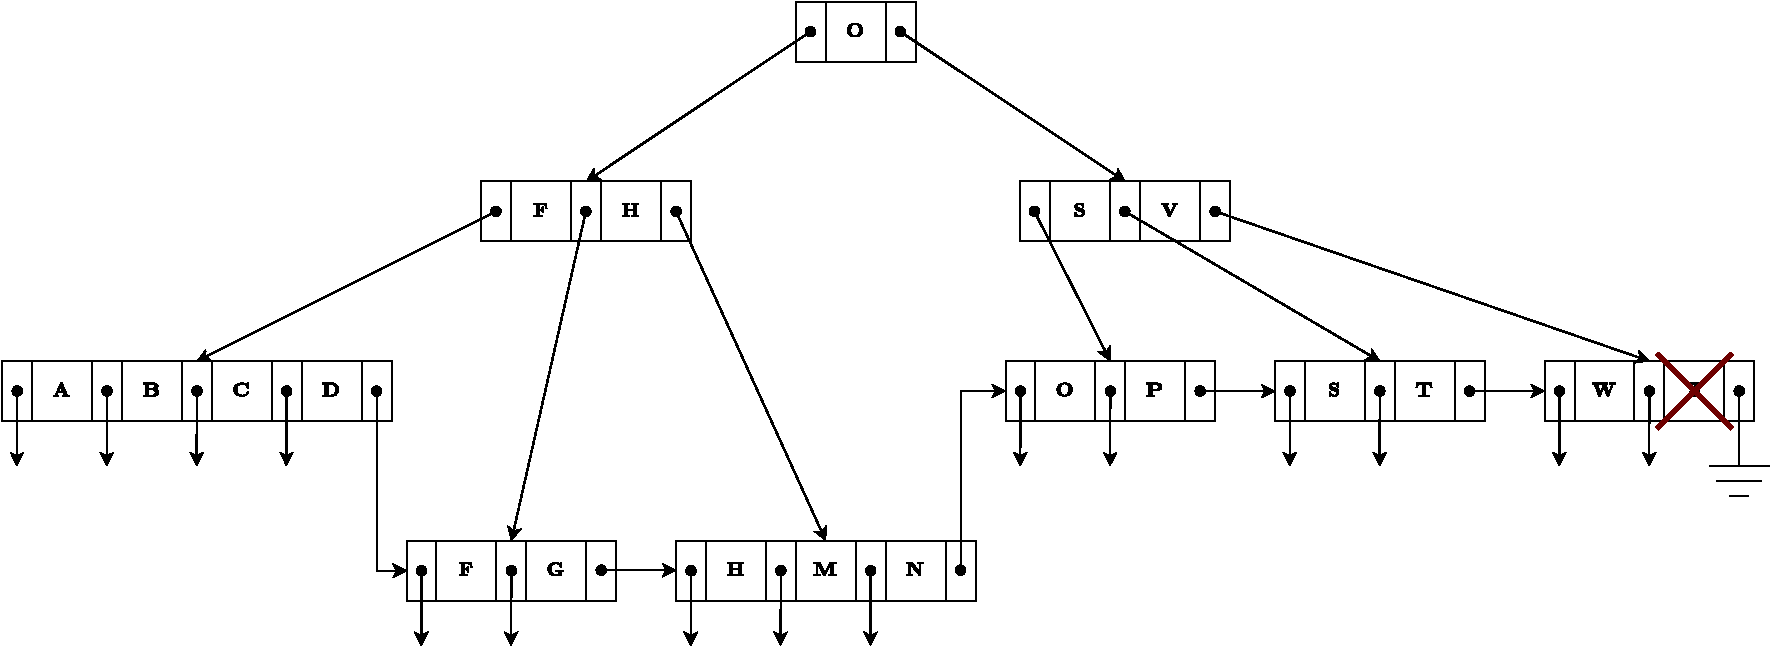
\includegraphics[width=\textwidth]{img/b+-tree-7.pdf}
		\caption*{Eliminazione della chiave Z.}
	\end{figure}
	
	\begin{figure}[!htp]
		\centering
		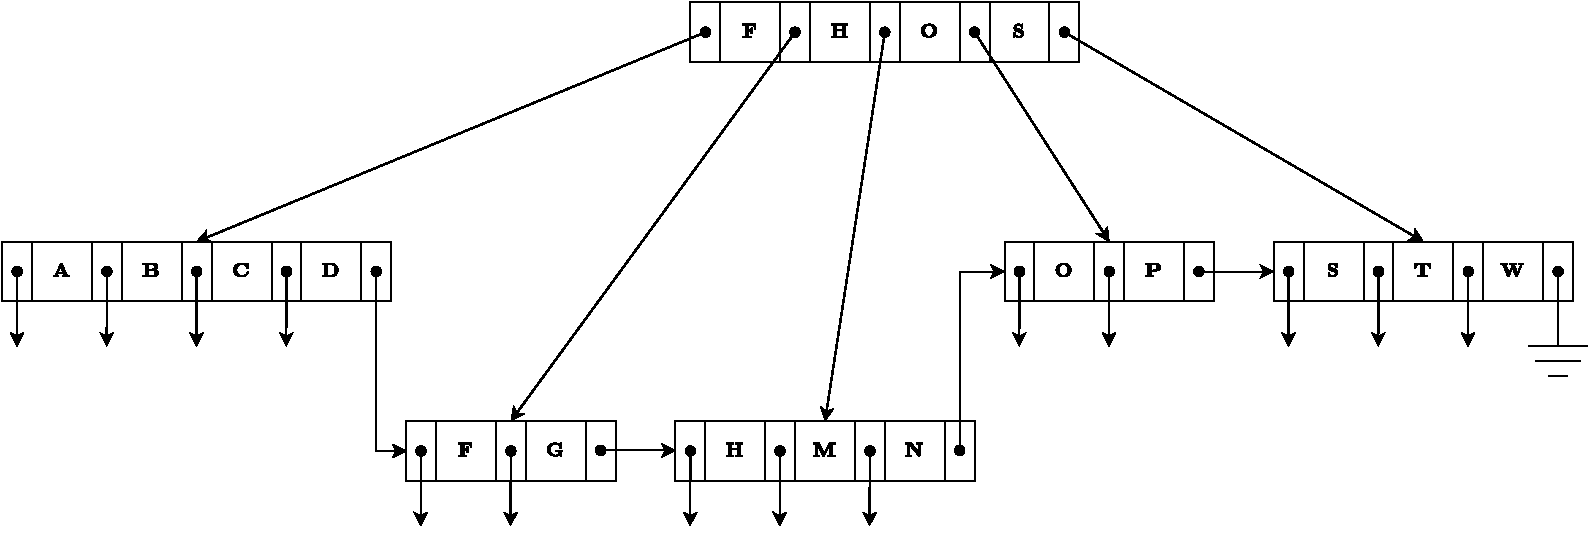
\includegraphics[width=\textwidth]{img/b+-tree-8.pdf}
		\caption*{Merge degli ultimi due nodi.}
	\end{figure}\newpage
	
	\subsubsection{Esercizio 2}
	
	Data la seguente lista di possibili valori chiave:
	\begin{equation*}
		\begin{array}{lll}
			L &=& (1,2,3,4,5,6,7,8,9,10,11,12,13,14,15,16,17,18,19,20,21,22,23,24,25, \\
			&& \phantom{(}26,27,28,29,30)
		\end{array}
	\end{equation*}
	Costruire un B+-tree (\emph{fan-out} = 5) che contenga i seguenti nodi foglia:
	\begin{figure}[!htp]
		\centering
		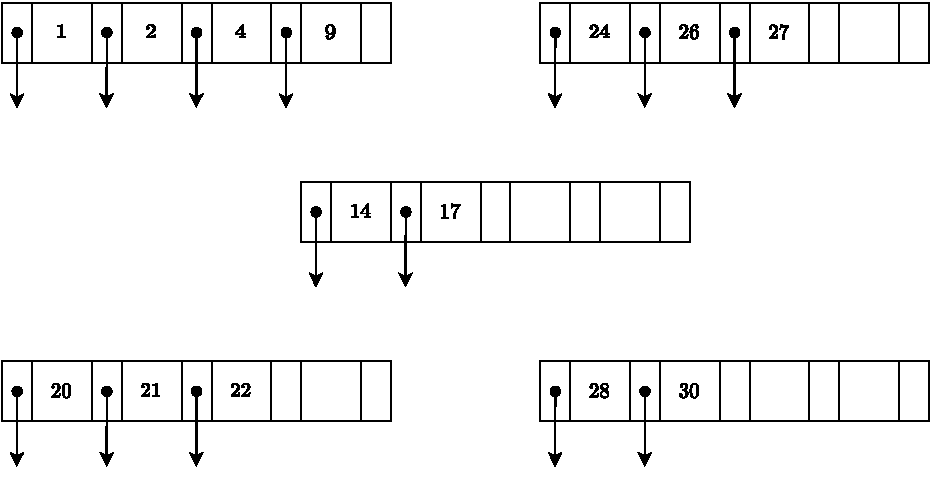
\includegraphics[width=\textwidth]{img/b+-tree-9.pdf}
	\end{figure}
	
	\noindent
	Mostrare l'albero dopo l'inserimento del valore chiave 5 e partendo da questo risultato, mostrare l'albero dopo la cancellazione del valore chiave 28.\newline
	
	\noindent
	\textcolor{Green4}{\textbf{\emph{\underline{Soluzione}}}}\newline
	
	\noindent
	Si costruisce la lista:
	\begin{figure}[!htp]
		\centering
		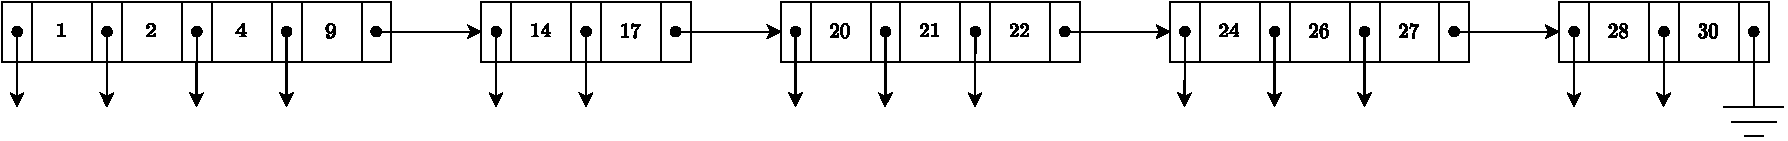
\includegraphics[width=\textwidth]{img/b+-tree-10.pdf}
	\end{figure}
	
	\noindent
	E poi l'albero:
	\begin{figure}[!htp]
		\centering
		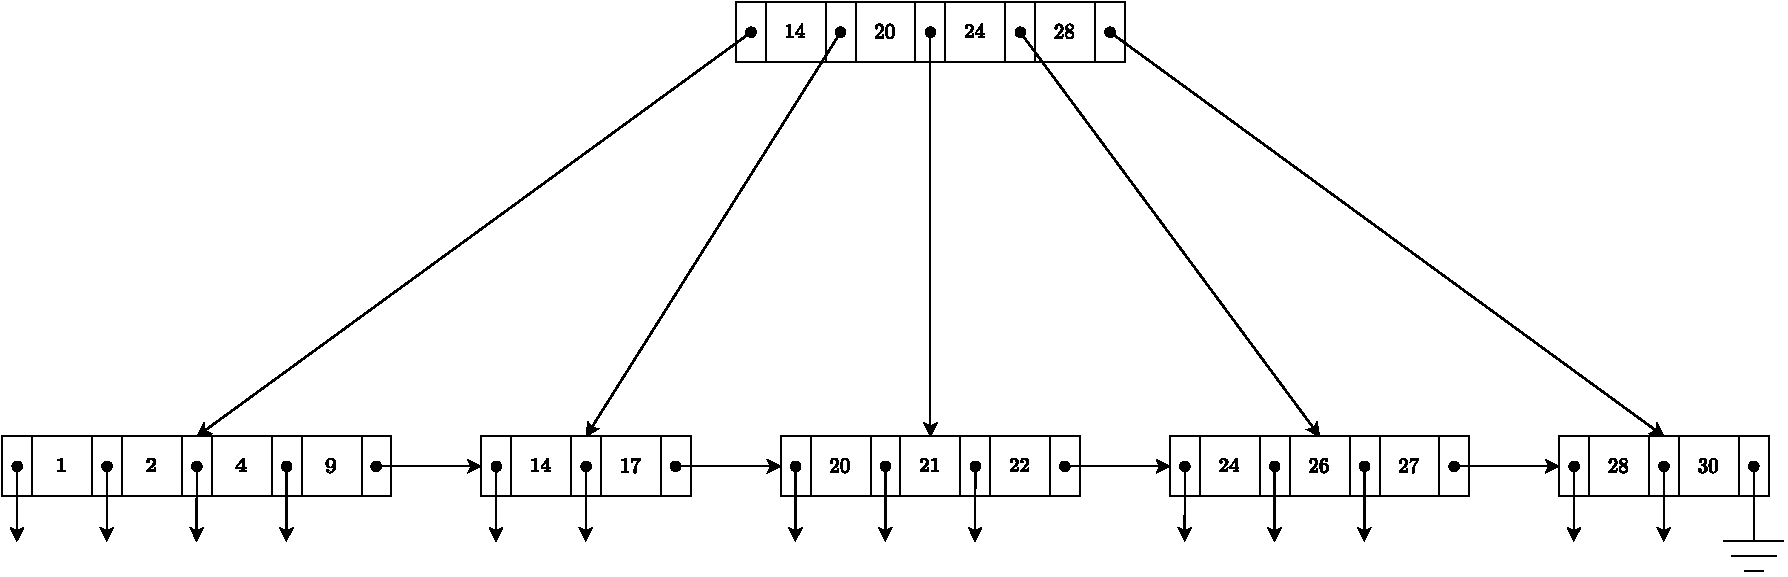
\includegraphics[width=\textwidth]{img/b+-tree-11.pdf}
	\end{figure}\newpage
	
	\noindent
	Si inserisce il valore 5:
	\begin{figure}[!htp]
		\centering
		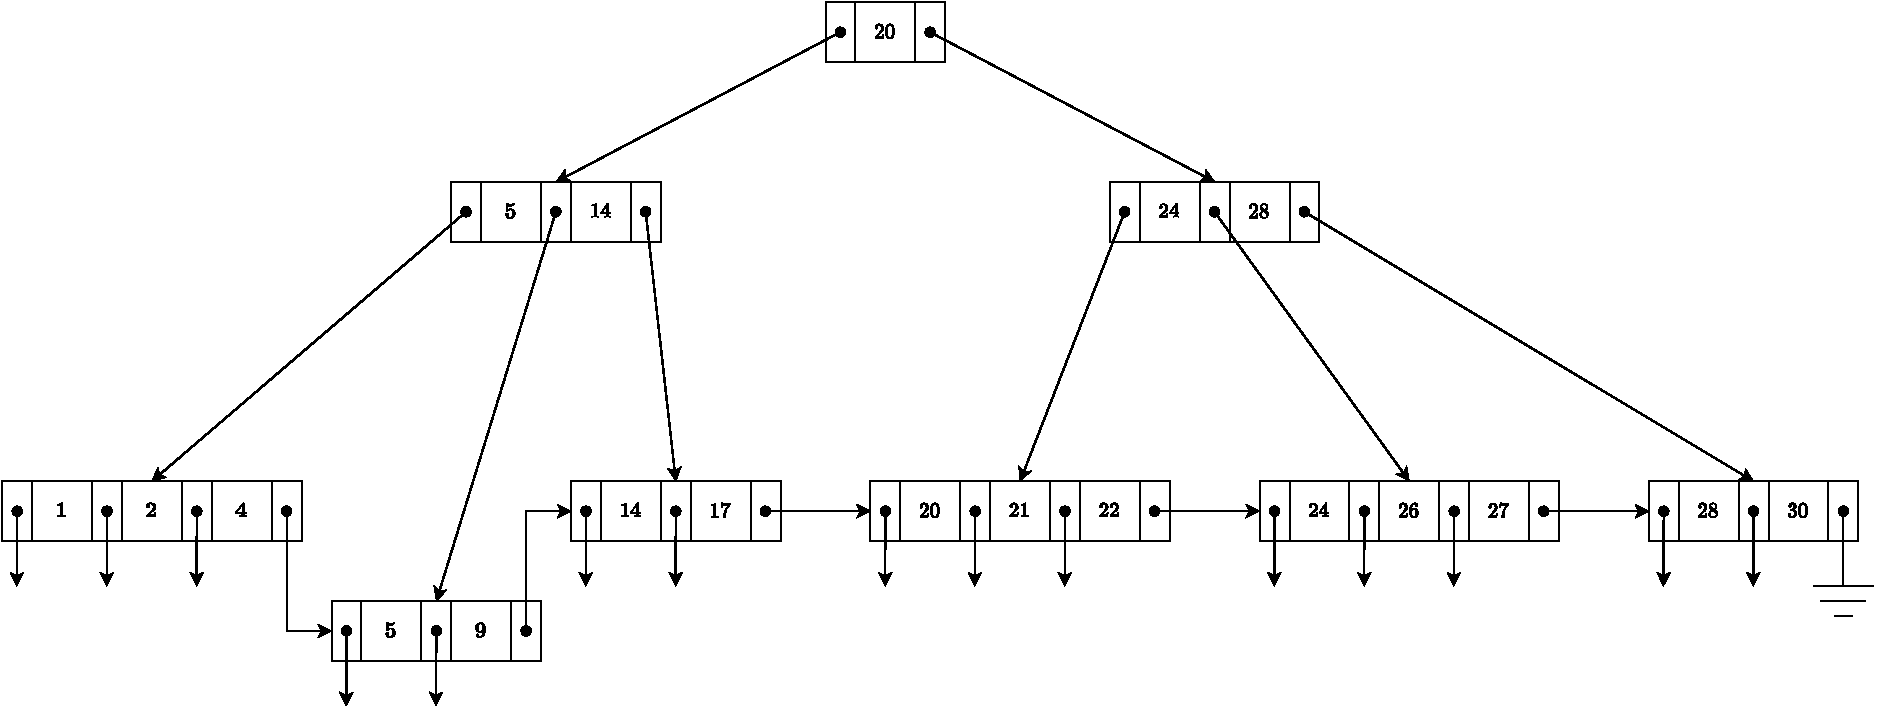
\includegraphics[width=\textwidth]{img/b+-tree-12.pdf}
	\end{figure}
	
	\noindent
	E infine si rimuove il valore 28:
	\begin{figure}[!htp]
		\centering
		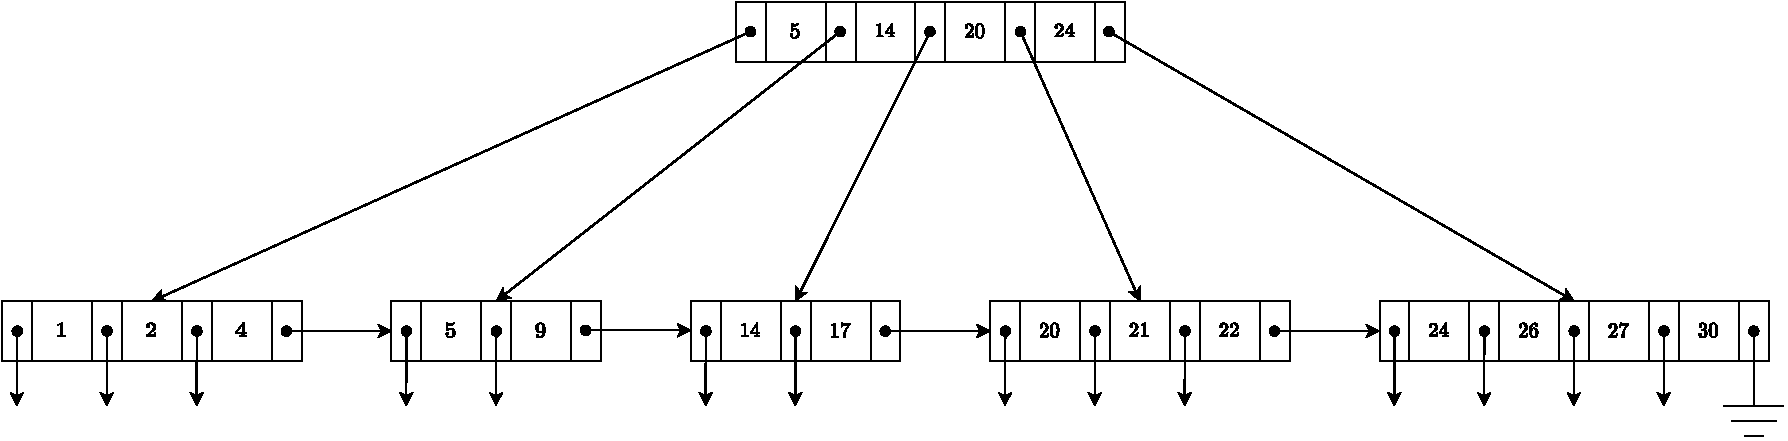
\includegraphics[width=\textwidth]{img/b+-tree-13.pdf}
	\end{figure}\newpage
	
	\subsection{Verificare che uno schedule sia VSR (View-serializzabile)}
	
	\subsubsection{Esercizio 1 - Perdita di aggiornamento}
	
	Date due transazioni $T_{1}$ e $T_{2}$ di seguito descritte:
	\begin{equation*}
		\begin{array}{lll}
			T_{1} &:& r_{1}\left(x\right) \: w_{1}\left(x\right) \\
			T_{2} &:& r_{2}\left(x\right) \: w_{2}\left(x\right)
		\end{array}
	\end{equation*}
	Lo schedule che rappresenta l'anomalia è il seguente:
	\begin{equation*}
		S_{PA} = r_{1}\left(x\right) \: r_{2}\left(x\right) \: w_{2}\left(x\right) \: w_{1}\left(x\right)
	\end{equation*}
	Per verificare che uno schedule sia VSR o meno, è necessario caratterizzare $S_{PA}$ calcolando l'insieme delle relazioni LeggeDa e l'insieme delle ScrittureFinali.\newline
	
	\noindent
	Quindi, per l'insieme LeggeDa viene cercato per ogni operazione di lettura, una precedente scrittura sulla stessa risorsa fatta da un'altra transazione. In questo caso, l'insieme è vuoto poiché nessuna risorsa scrive prime di una lettura.\newline
	
	\noindent
	Invece, per l'insieme ScrittureFinali, per ogni risorsa indicata nello schedule si specifica l'ultima scrittura eseguita. In questo caso, l'unica risorsa è $x$ e l'ultima scrittura è $w_{1}\left(x\right)$.\newline
	
	\noindent
	Quindi, gli insiemi sono composti da:
	\begin{equation*}
		\begin{array}{rll}
			\text{LeggeDa}\left(S_{PA}\right) &=& \emptyset \\
			\text{ScrittureFinali}\left(S_{PA}\right) &=& \left\{w_{1}\left(x\right)\right\}
		\end{array}
	\end{equation*}
	Adesso si generano tutti i possibili schedule seriali che eseguono le due transazioni. Essi si ottengono generando le possibili permutazioni dell'insieme di transazioni che partecipano allo schedule. In questo caso, date solo due transazioni $T_{1}$ e $T_{2}$, le possibili combinazioni sono:
	\begin{equation*}
		\begin{array}{lllll}
			S_{1} &=& T_{1} \: T_{2} &=& r_{1}\left(x\right) \: w_{1}\left(x\right) \: r_{2}\left(x\right) \: w_{2}\left(x\right) \\
			S_{2} &=& T_{2} \: T_{1} &=& r_{2}\left(x\right) \: w_{2}\left(x\right) \: r_{1}\left(x\right) \: w_{1}\left(x\right) \\
		\end{array}
	\end{equation*}
	Adesso, si verifica che almeno uno dei due schedule seriali è view-equivalente a $S_{PA}$.\newpage
	
	\noindent
	Verifica partendo dallo schedule $S_{1}$:
	\begin{enumerate}
		\item Creazione dell'insieme LeggeDa$\left(S_{1}\right)$. Data la sequenza:
		\begin{equation*}
			S_{1} = r_{1}\left(x\right) \: w_{1}\left(x\right) \: r_{2}\left(x\right) \: w_{2}\left(x\right)
		\end{equation*}
		L'unica scrittura che precede una lettura è $w_{1}\left(x\right)$. Quindi, l'insieme è composto dalla scrittura che avviene prima della lettura e da quest'ultima:
		\begin{equation*}
			\text{LeggeDa}\left(S_{1}\right) = \left\{\left(r_{2}\left(x\right), w_{1}\left(x\right)\right)\right\}
		\end{equation*}
		
		\item Creazione dell'insieme ScrittureFinali$\left(S_{1}\right)$. Data la sequenza:
		\begin{equation*}
			S_{1} = r_{1}\left(x\right) \: w_{1}\left(x\right) \: r_{2}\left(x\right) \: w_{2}\left(x\right)
		\end{equation*}
		L'unica risorsa $x$ ha come ultima scrittura $w_{2}\left(x\right)$, quindi l'insieme è composto da:
		\begin{equation*}
			\text{ScrittureFinali}\left(S_{1}\right) = \left\{w_{2}\left(x\right)\right\}
		\end{equation*}
		
		\item Si esegue il confronto degli insiemi ottenuti da $S_{1}$ e dagli insiemi ottenuti da $S_{PA}$:
		\begin{equation*}
			\begin{array}{lll}
				\text{LeggeDa}\left(S_{PA}\right)	&=& \emptyset \\
				\text{LeggeDa}\left(S_{1}\right)	&=& \left\{\left(r_{2}\left(x\right), w_{1}\left(x\right)\right)\right\} \\
				\text{ScrittureFinali}\left(S_{PA}\right)	&=& \left\{w_{1}\left(x\right)\right\} \\
				\text{ScrittureFinali}\left(S_{1}\right)	&=& \left\{w_{2}\left(x\right)\right\}
			\end{array}
		\end{equation*}
		Come è evidente, nessuno dei due insiemi è equivalente:
		\begin{equation*}
			\begin{array}{lll}
				\text{LeggeDa}\left(S_{PA}\right)	&\cancel{\equiv}& \text{LeggeDa}\left(S_{1}\right) \\
				\text{ScrittureFinali}\left(S_{PA}\right)	&\cancel{\equiv}& \text{ScrittureFinali}\left(S_{1}\right)
			\end{array}
		\end{equation*}
		Quindi, è possibile concludere che $S_{PA}$ non è view-equivalente a $S_{1}$.
	\end{enumerate}\newpage
	
	\noindent
	Verifica partendo dallo schedule $S_{2}$:
	\begin{enumerate}
		\item Creazione dell'insieme LeggeDa$\left(S_{2}\right)$. Data la sequenza:
		\begin{equation*}
			S_{2} = r_{2}\left(x\right) \: w_{2}\left(x\right) \: r_{1}\left(x\right) \: w_{1}\left(x\right)
		\end{equation*}
		L'unica scrittura che precede una lettura è $w_{2}\left(x\right)$. Quindi, l'insieme è composto dalla scrittura che avviene prima della lettura e da quest'ultima:
		\begin{equation*}
			\text{LeggeDa}\left(S_{2}\right) = \left\{\left(r_{1}\left(x\right), w_{2}\left(x\right)\right)\right\}
		\end{equation*}
		
		\item Creazione dell'insieme ScrittureFinali$\left(S_{2}\right)$. Data la sequenza:
		\begin{equation*}
			S_{2} = r_{2}\left(x\right) \: w_{2}\left(x\right) \: r_{1}\left(x\right) \: w_{1}\left(x\right)
		\end{equation*}
		L'unica risorsa $x$ ha come ultima scrittura $w_{2}\left(x\right)$, quindi l'insieme è composto da:
		\begin{equation*}
			\text{ScrittureFinali}\left(S_{2}\right) = \left\{w_{1}\left(x\right)\right\}
		\end{equation*}
		
		\item Si esegue il confronto degli insiemi ottenuti da $S_{1}$ e dagli insiemi ottenuti da $S_{PA}$:
		\begin{equation*}
			\begin{array}{lll}
				\text{LeggeDa}\left(S_{PA}\right)	&=& \emptyset \\
				\text{LeggeDa}\left(S_{1}\right)	&=& \left\{\left(r_{1}\left(x\right), w_{2}\left(x\right)\right)\right\} \\
				\text{ScrittureFinali}\left(S_{PA}\right)	&=& \left\{w_{1}\left(x\right)\right\} \\
				\text{ScrittureFinali}\left(S_{1}\right)	&=& \left\{w_{1}\left(x\right)\right\}
			\end{array}
		\end{equation*}
		Come è evidente, soltanto uno dei due insiemi è equivalente:
		\begin{equation*}
			\begin{array}{lll}
				\text{LeggeDa}\left(S_{PA}\right)	&\cancel{\equiv}& \text{LeggeDa}\left(S_{1}\right) \\
				\text{ScrittureFinali}\left(S_{PA}\right)	&\equiv& \text{ScrittureFinali}\left(S_{1}\right)
			\end{array}
		\end{equation*}
		Quindi, è possibile concludere che $S_{PA}$ non è view-equivalente a $S_{1}$ poiché entrambi gli insiemi non sono equivalenti.
	\end{enumerate}
	L'esercizio si conclude qua. Nessuna combinazione è view-equivalente allo schedule di partenza $S_{PA}$. Quindi, si conclude affermando che $S_{PA}$ non è VSR.\newpage
	
	\subsubsection{Esercizio 2 - Lettura inconsistente}
	
	Date due transazioni $T_{1}$ e $T_{2}$ di seguito descritte:
	\begin{equation*}
		\begin{array}{lll}
			T_{1} &:& r_{1}\left(x\right) \: r_{1}'\left(x\right) \\
			T_{2} &:& r_{2}\left(x\right) \: w_{2}\left(x\right)
		\end{array}
	\end{equation*}
	Lo schedule che rappresenta l'anomalia è il seguente:
	\begin{equation*}
		S_{LI} = r_{1}\left(x\right) \: r_{2}\left(x\right) \: w_{2}\left(x\right) \: r_{1}'\left(x\right)
	\end{equation*}
	Per verificare che uno schedule sia VSR o meno, è necessario caratterizzare $S_{LI}$ calcolando l'insieme delle relazioni LeggeDa e l'insieme delle ScrittureFinali.\newline
	
	\noindent
	Quindi, per l'insieme LeggeDa viene cercato per ogni operazione di lettura, una precedente scrittura sulla stessa risorsa fatta da un'altra transazione. In questo caso, l'insieme è composto da $w_{2}\left(x\right)$ perché precede $r_{1}'\left(x\right)$.\newline
	
	\noindent
	Invece, per l'insieme ScrittureFinali, per ogni risorsa indicata nello schedule si specifica l'ultima scrittura eseguita. In questo caso, l'unica risorsa è $x$ e l'ultima scrittura è $w_{2}\left(x\right)$.\newline
	
	\noindent
	Quindi, gli insiemi sono composti da:
	\begin{equation*}
		\begin{array}{rll}
			\text{LeggeDa}\left(S_{LI}\right) &=& \left\{\left(r_{1}'\left(x\right), w_{2}\left(x\right)\right)\right\} \\
			\text{ScrittureFinali}\left(S_{LI}\right) &=& \left\{w_{2}\left(x\right)\right\}
		\end{array}
	\end{equation*}
	Adesso si generano tutti i possibili schedule seriali che eseguono le due transazioni. Essi si ottengono generando le possibili permutazioni dell'insieme di transazioni che partecipano allo schedule. In questo caso, date solo due transazioni $T_{1}$ e $T_{2}$, le possibili combinazioni sono:
	\begin{equation*}
		\begin{array}{lllll}
			S_{1} &=& T_{1} \: T_{2} &=& r_{1}\left(x\right) \: r_{1}'\left(x\right) \: r_{2}\left(x\right) \: w_{2}\left(x\right) \\
			S_{2} &=& T_{2} \: T_{1} &=& r_{2}\left(x\right) \: w_{2}\left(x\right) \: r_{1}\left(x\right) \: r_{1}'\left(x\right) \\
		\end{array}
	\end{equation*}
	Adesso, si verifica che almeno uno dei due schedule seriali è view-equivalente a $S_{LI}$.\newpage
	
	\noindent
	Verifica partendo dallo schedule $S_{1}$:
	\begin{enumerate}
		\item Creazione dell'insieme LeggeDa$\left(S_{1}\right)$. Data la sequenza:
		\begin{equation*}
			S_{1} = r_{1}\left(x\right) \: r_{1}'\left(x\right) \: r_{2}\left(x\right) \: w_{2}\left(x\right)
		\end{equation*}
		L'unica scrittura che precede una lettura è $w_{1}\left(x\right)$. Quindi, l'insieme è composto dalla scrittura che avviene prima della lettura e da quest'ultima:
		\begin{equation*}
			\text{LeggeDa}\left(S_{1}\right) = \emptyset
		\end{equation*}
		
		\item Creazione dell'insieme ScrittureFinali$\left(S_{1}\right)$. Data la sequenza:
		\begin{equation*}
			S_{1} = r_{1}\left(x\right) \: r_{1}'\left(x\right) \: r_{2}\left(x\right) \: w_{2}\left(x\right)
		\end{equation*}
		L'unica risorsa $x$ ha come ultima scrittura $w_{2}\left(x\right)$, quindi l'insieme è composto da:
		\begin{equation*}
			\text{ScrittureFinali}\left(S_{1}\right) = \left\{w_{2}\left(x\right)\right\}
		\end{equation*}
		
		\item Si esegue il confronto degli insiemi ottenuti da $S_{1}$ e dagli insiemi ottenuti da $S_{LI}$:
		\begin{equation*}
			\begin{array}{lll}
				\text{LeggeDa}\left(S_{LI}\right)	&=& \left\{\left(r_{1}'\left(x\right), w_{2}\left(x\right)\right)\right\} \\
				\text{LeggeDa}\left(S_{1}\right)	&=& \emptyset \\
				\text{ScrittureFinali}\left(S_{LI}\right)	&=& \left\{w_{2}\left(x\right)\right\} \\
				\text{ScrittureFinali}\left(S_{1}\right)	&=& \left\{w_{2}\left(x\right)\right\}
			\end{array}
		\end{equation*}
		Come è evidente, soltanto uno dei due insiemi è equivalente:
		\begin{equation*}
			\begin{array}{lll}
				\text{LeggeDa}\left(S_{LI}\right)	&\cancel{\equiv}& \text{LeggeDa}\left(S_{1}\right) \\
				\text{ScrittureFinali}\left(S_{LI}\right)	&\equiv& \text{ScrittureFinali}\left(S_{1}\right)
			\end{array}
		\end{equation*}
		Quindi, è possibile concludere che $S_{LI}$ non è view-equivalente a $S_{1}$.
	\end{enumerate}\newpage
	
	\noindent
	Verifica partendo dallo schedule $S_{2}$:
	\begin{enumerate}
		\item Creazione dell'insieme LeggeDa$\left(S_{2}\right)$. Data la sequenza:
		\begin{equation*}
			S_{2} = r_{2}\left(x\right) \: w_{2}\left(x\right) \: r_{1}\left(x\right) \: r_{1}'\left(x\right)
		\end{equation*}
		L'unica scrittura che precede due letture è $w_{2}\left(x\right)$. Quindi, l'insieme è composto dalla scrittura che avviene con due letture:
		\begin{equation*}
			\text{LeggeDa}\left(S_{2}\right) = \left\{\left(r_{1}'\left(x\right), w_{2}\left(x\right)\right), \left(r_{1}\left(x\right), w_{2}\left(x\right)\right)\right\}
		\end{equation*}
		
		\item Creazione dell'insieme ScrittureFinali$\left(S_{2}\right)$. Data la sequenza:
		\begin{equation*}
			S_{2} = r_{2}\left(x\right) \: w_{2}\left(x\right) \: r_{1}\left(x\right) \: r_{1}'\left(x\right)
		\end{equation*}
		L'unica risorsa $x$ ha come ultima scrittura $w_{2}\left(x\right)$, quindi l'insieme è composto da:
		\begin{equation*}
			\text{ScrittureFinali}\left(S_{2}\right) = \left\{w_{2}\left(x\right)\right\}
		\end{equation*}
		
		\item Si esegue il confronto degli insiemi ottenuti da $S_{1}$ e dagli insiemi ottenuti da $S_{PA}$:
		\begin{equation*}
			\begin{array}{lll}
				\text{LeggeDa}\left(S_{LI}\right)	&=& \left\{\left(r_{1}'\left(x\right), w_{2}\left(x\right)\right)\right\} \\
				\text{LeggeDa}\left(S_{2}\right)	&=& \left\{\left(r_{1}'\left(x\right), w_{2}\left(x\right)\right), \left(r_{1}\left(x\right), w_{2}\left(x\right)\right)\right\} \\
				\text{ScrittureFinali}\left(S_{LI}\right)	&=& \left\{w_{2}\left(x\right)\right\} \\
				\text{ScrittureFinali}\left(S_{2}\right)	&=& \left\{w_{2}\left(x\right)\right\}
			\end{array}
		\end{equation*}
		Come è evidente, soltanto uno dei due insiemi è equivalente:
		\begin{equation*}
			\begin{array}{lll}
				\text{LeggeDa}\left(S_{PA}\right)	&\cancel{\equiv}& \text{LeggeDa}\left(S_{1}\right) \\
				\text{ScrittureFinali}\left(S_{PA}\right)	&\equiv& \text{ScrittureFinali}\left(S_{1}\right)
			\end{array}
		\end{equation*}
		Quindi, è possibile concludere che $S_{LI}$ non è view-equivalente a $S_{2}$ poiché entrambi gli insiemi non sono equivalenti.
	\end{enumerate}
	L'esercizio si conclude qua. Nessuna combinazione è view-equivalente allo schedule di partenza $S_{LI}$. Quindi, si conclude affermando che $S_{LI}$ non è VSR.\newpage
	
	\subsubsection{Sintesi dell'algoritmo}
	
	In sintesi l'algoritmo per capire se uno schedule è VSR:
	\begin{enumerate}
		\item Si tiene bene in considerazione lo schedule che rappresenta l'anomalia, ovvero quello che viene dato;
		
		\item Si compongono i due insiemi:
		\begin{enumerate}
			\item Creazione insieme LeggeDa cercando per ogni operazione di lettura ($r_{i}\left(\text{risorsa}\right)$) una precedente operazione di scrittura sulla stessa risorsa fatta da un'altra transazione. Nel caso in cui si trovi, si aggiunge all'insieme la scrittura incriminata e la relativa lettura;
			
			\item Creazione insieme ScrittureFinali cercando per ogni risorsa indicata nello schedule l'ultima scrittura eseguita.
		\end{enumerate}
		
		\item Date le varie transazioni, si creano tutti i possibili schedule creando così una lista;
		
		\item Si verifica che almeno uno schedule della lista sia view-equivalente allo schedule dato al punto 1. Per farlo si esegue questo piccolo algoritmo:
		\begin{enumerate}
			\item Creazione dell'insieme LeggeDa (vedi punto 2.a);
			
			\item Creazione dell'insieme ScrittureFinali (vedi punto 2.b);
			
			\item Confronto degli insiemi creati precedente con quelli creati per lo schedule dato al punto 1. Se non sono uguali tutti uguali, allora lo schedule creato tramite combinazione non è equivalente allo schedule dato al punto 1. Altrimenti, è possibile affermare di aver trovato una combinazione view-equivalente.
		\end{enumerate}
		
		\item Al termine della creazione degli insiemi e dei vari confronti, se esiste almeno una combinazione che è view-equivalente allo schedule del punto 1, allora è possibile affermare che lo schedule di partenza è VSR.
	\end{enumerate}\newpage
	
	\subsection{Verificare che uno schedule sia CSR (Conflict-serializzabile)}
	
	\subsubsection{Esercizio 1 - Perdita di aggiornamento}
	
	Date due transizioni $T_{1}$ e $T_{2}$:
	\begin{equation*}
		\begin{array}{lll}
			T_{1} &:& r_{1}\left(x\right) \: w_{1}\left(x\right) \\
			T_{2} &:& r_{2}\left(x\right) \: w_{2}\left(x\right)
		\end{array}
	\end{equation*}
	Lo schedule che rappresenta l'anomalia è il seguente:
	\begin{equation*}
		S_{PA} = r_{1}\left(x\right) \: r_{2}\left(x\right) \: w_{2}\left(x\right) \: w_{1}\left(x\right)
	\end{equation*}
	Per verificare CSR è necessario caratterizzare $S_{PA}$ calcolando l'insieme dei conflitti. Si ricorda che due azioni sono in conflitto se operano sullo stesso oggetto e se almeno una di esse è in scrittura (quindi le combinazioni: $rw, wr, ww$). Quindi, si calcola l'insieme dei conflitti di $S_{PA}$:
	\begin{enumerate}
		\item $\textcolor{Red3}{r_{1}\left(x\right)} \: r_{2}\left(x\right) \: \textcolor{Red3}{w_{2}\left(x\right)} \: w_{1}\left(x\right)$
		
		\item $r_{1}\left(x\right) \: \textcolor{Red3}{r_{2}\left(x\right)} \: w_{2}\left(x\right) \: \textcolor{Red3}{w_{1}\left(x\right)}$
		
		\item $r_{1}\left(x\right) \: r_{2}\left(x\right) \: \textcolor{Red3}{w_{2}\left(x\right)} \: \textcolor{Red3}{w_{1}\left(x\right)}$
	\end{enumerate}
	L'insieme è quindi così costituito:
	\begin{equation*}
		\text{Conflitti}\left(S_{PA}\right) = \left\{\left(r_{1}\left(x\right), w_{2}\left(x\right)\right), \left(r_{2}\left(x\right), w_{1}\left(x\right)\right), \left(w_{2}\left(x\right), w_{1}\left(x\right)\right)\right\}
	\end{equation*}
	Si costruisce il grafo nel seguente modo. Si rappresentano tanti nodi quanti sono le transazioni e ogni arco (orientato) viene tracciato da $t_{i}$ a $t_{j}$ se vengono rispettate due condizioni: se c'è almeno un conflitto fra un'azione $a_{i}$ e un'azione $a_{j}$ tale che $a_{i}$ precede $a_{j}$. Quindi:
	\begin{figure}[!htp]
		\centering
		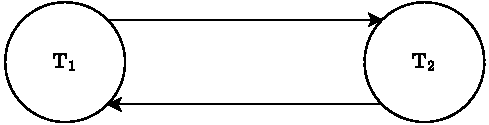
\includegraphics[width=.55\textwidth]{img/CSR-1.pdf}
	\end{figure}
	
	\noindent
	Se il grafo è aciclico allora $S_{PA}$ è CSR. In questo caso, il grafo non è aciclico ma ciclico, per cui $S_{PA}$ non è CSR.\newpage
	
	\subsubsection{Esercizio 2 - Lettura inconsistente}
	
	Date due transizioni $T_{1}$ e $T_{2}$:
	\begin{equation*}
		\begin{array}{lll}
			T_{1} &:& r_{1}\left(x\right) \: r_{1}'\left(x\right) \\
			T_{2} &:& r_{2}\left(x\right) \: w_{2}\left(x\right)
		\end{array}
	\end{equation*}
	Lo schedule che rappresenta l'anomalia è il seguente:
	\begin{equation*}
		S_{LI} = r_{1}\left(x\right) \: r_{2}\left(x\right) \: w_{2}\left(x\right) \: r_{1}'\left(x\right)
	\end{equation*}
	Per verificare CSR è necessario caratterizzare $S_{LI}$ calcolando l'insieme dei conflitti. Si ricorda che due azioni sono in conflitto se operano sullo stesso oggetto e se almeno una di esse è in scrittura (quindi le combinazioni: $rw, wr, ww$). Quindi, si calcola l'insieme dei conflitti di $S_{LI}$:
	\begin{enumerate}
		\item $\textcolor{Red3}{r_{1}\left(x\right)} \: r_{2}\left(x\right) \: \textcolor{Red3}{w_{2}\left(x\right)} \: r_{1}'\left(x\right)$
		
		\item $r_{1}\left(x\right) \: r_{2}\left(x\right) \: \textcolor{Red3}{w_{2}\left(x\right)} \: \textcolor{Red3}{r_{1}'\left(x\right)}$
	\end{enumerate}
	L'insieme è quindi così costituito:
	\begin{equation*}
		\text{Conflitti}\left(S_{LI}\right) = \left\{\left(r_{1}\left(x\right), w_{2}\left(x\right)\right), \left(w_{2}\left(x\right), r_{1}'\left(x\right)\right)\right\}
	\end{equation*}
	Si costruisce il grafo nel seguente modo. Si rappresentano tanti nodi quanti sono le transazioni e ogni arco (orientato) viene tracciato da $t_{i}$ a $t_{j}$ se vengono rispettate due condizioni: se c'è almeno un conflitto fra un'azione $a_{i}$ e un'azione $a_{j}$ tale che $a_{i}$ precede $a_{j}$. Quindi:
	\begin{figure}[!htp]
		\centering
		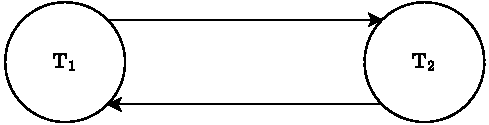
\includegraphics[width=.55\textwidth]{img/CSR-1.pdf}
	\end{figure}
	
	\noindent
	Se il grafo è aciclico allora $S_{LI}$ è CSR. In questo caso, il grafo non è aciclico ma ciclico, per cui $S_{LI}$ non è CSR.
	
	\longline
	
	\subsubsection{Sintesi dell'algoritmo}
	
	In sintesi l'algoritmo per capire se uno schedule è CSR:
	\begin{enumerate}
		\item Si calcola l'insieme dei conflitti. Un conflitto si manifesta quando due azioni \textbf{differenti} operano sullo stesso oggetto e quando almeno una di esse è in scrittura. Quindi, le combinazioni che possono esserci sono: $rw, wr, ww$;
		
		\item Si costruire il grafo dall'insieme dei conflitti. I nodi rappresentano le transizioni e gli archi si disegnano solo se due azioni non riguardano la stessa transizione.
	\end{enumerate}\newpage
	
	\subsection{Verificare che uno schedule sia NonSR, VSR e/o CSR}
	
	\subsubsection{Testo esercizio}
	
	Classificare i seguenti schedule (come: NonSR, VSR, CSR); nel caso uno schedule sia VSR oppure CSR, indicare tutti gli schedule seriali a esso equivalenti.
	\begin{enumerate}
		\item $S_{1} = r_{1}\left(x\right) \: w_{1}\left(x\right) \: r_{2}\left(z\right) \: r_{1}\left(y\right) \: w_{1}\left(y\right) \: r_{2}\left(x\right) \: w_{2}\left(x\right) \: w_{2}\left(z\right)$
		
		\item $S_{2} = r_{1}\left(x\right) \: w_{1}\left(x\right) \: w_{3}\left(x\right) \: r_{2}\left(y\right) \: r_{3}\left(y\right) \: w_{3}\left(y\right) \: w_{1}\left(y\right) \: r_{2}\left(x\right)$
		
		\item $S_{3} = r_{1}\left(x\right) \: r_{2}\left(x\right) \: w_{2}\left(x\right) \: r_{3}\left(x\right) \: r_{4}\left(z\right) \: w_{1}\left(x\right) \: w_{3}\left(y\right) \: w_{3}\left(x\right) \: w_{1}\left(y\right) \: w_{5}\left(x\right) \: w_{1}\left(z\right) \: w_{5}\left(y\right) \: r_{5}\left(z\right)$
		
		\item $S_{4} = r_{1}\left(x\right) \: r_{3}\left(y\right) \: w_{1}\left(y\right) \: w_{4}\left(x\right) \: w_{1}\left(t\right) \: w_{5}\left(x\right) \: r_{2}\left(z\right) \: r_{3}\left(z\right) \: w_{2}\left(z\right) \: w_{5}\left(z\right) \: r_{4}\left(t\right) \: r_{5}\left(t\right)$
	\end{enumerate}
	
	\longline
	
	\subsubsection{Schedule 1}
	
	Dato il seguente schedule:
	\begin{equation*}
		S_{1} = r_{1}\left(x\right) \: w_{1}\left(x\right) \: r_{2}\left(z\right) \: r_{1}\left(y\right) \: w_{1}\left(y\right) \: r_{2}\left(x\right) \: w_{2}\left(x\right) \: w_{2}\left(z\right)
	\end{equation*}
	Le transizioni sono:
	\begin{equation*}
		\begin{array}{lll}
			T_{1} &:& r_{1}\left(x\right) \: w_{1}\left(x\right) \: r_{1}\left(y\right) \: w_{1}\left(y\right) \\
			T_{2} &:& r_{2}\left(z\right) \: r_{2}\left(x\right) \: w_{2}\left(x\right) \: w_{2}\left(z\right)
		\end{array}
	\end{equation*}
	Si verifica se è CSR. Quindi, si crea l'insieme dei conflitti:
	\begin{enumerate}
		\item $\textcolor{Red3}{r_{1}\left(x\right)} \: w_{1}\left(x\right) \: r_{2}\left(z\right) \: r_{1}\left(y\right) \: w_{1}\left(y\right) \: r_{2}\left(x\right) \: \textcolor{Red3}{w_{2}\left(x\right)} \: w_{2}\left(z\right)$
		
		\item $r_{1}\left(x\right) \: \textcolor{Red3}{w_{1}\left(x\right)} \: r_{2}\left(z\right) \: r_{1}\left(y\right) \: w_{1}\left(y\right) \: \textcolor{Red3}{r_{2}\left(x\right)} \: w_{2}\left(x\right) \: w_{2}\left(z\right)$
		
		\item $r_{1}\left(x\right) \: \textcolor{Red3}{w_{1}\left(x\right)} \: r_{2}\left(z\right) \: r_{1}\left(y\right) \: w_{1}\left(y\right) \: r_{2}\left(x\right) \: \textcolor{Red3}{w_{2}\left(x\right)} \: w_{2}\left(z\right)$
	\end{enumerate}
	Quindi l'insieme è:
	\begin{equation*}
		\text{Conflitti}\left(S_{1}\right) = \left\{\left(r_{1}\left(x\right) \: w_{2}\left(x\right)\right), \left(w_{1}\left(x\right) \: r_{2}\left(x\right)\right), \left(w_{1}\left(x\right) \: w_{2}\left(x\right)\right)\right\}
	\end{equation*}
	Si costruisce il grafo:
	\begin{figure}[!htp]
		\centering
		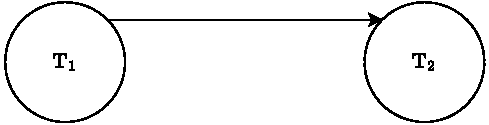
\includegraphics[width=.55\textwidth]{img/NoSR-VSR-CSR-1.pdf}
	\end{figure}
	
	\noindent
	Il ciclo è aciclico quindi è $S_{1}$ è CSR. Dato che CSR $\subset$ VSR, allora $S_{1}$ è anche VSR.\newpage
	
	\subsubsection{Schedule 2}
	
	Dato il seguente schedule:
	\begin{equation*}
		S_{2} = r_{1}\left(x\right) \: w_{1}\left(x\right) \: w_{3}\left(x\right) \: r_{2}\left(y\right) \: r_{3}\left(y\right) \: w_{3}\left(y\right) \: w_{1}\left(y\right) \: r_{2}\left(x\right)
	\end{equation*}
	Le transazioni sono:
	\begin{equation*}
		\begin{array}{lll}
			T_{1} &:& r_{1}\left(x\right) \: w_{1}\left(x\right) \: w_{1}\left(y\right) \\
			T_{2} &:& r_{2}\left(y\right) \: r_{2}\left(x\right) \\
			T_{3} &:& w_{3}\left(x\right) \: r_{3}\left(y\right) \: w_{3}\left(y\right)
		\end{array}
	\end{equation*}
	Si verifica se è VSR. Si inizia analizzando l'insieme $S_{2}$:
	\begin{equation*}
		\begin{array}{lll}
			\text{LeggeDa}\left(S_{2}\right) 			&=& \left\{\left(r_{2}\left(x\right), w_{3}\left(x\right)\right)\right\} \\
			\text{ScrittureFinali}\left(S_{2}\right) 	&=& \left\{w_{3}\left(x\right), w_{1}\left(y\right)\right\}
		\end{array}
	\end{equation*}
	Dato che è impossibile provare tutte le combinazioni (3 transazioni e quindi $3! = 6$), si fanno alcune considerazioni. Per esempio, dato che nelle LeggeDa si deve mantenere l'ordine $\left(r_{2}\left(x\right), w_{3}\left(x\right)\right)$, e sapendo che $r_{2}$ appartiene a $T_{2}$ e $w_{3}$ a $T_{3}$, si può concludere che $T_{3}$ deve per forza precedere $T_{2}$. Quindi, le combinazioni si riducono a:
	\begin{itemize}
		\item $T_{1} \: T_{3} \: T_{2}$
		
		\item $T_{3} \: T_{1} \: T_{2}$
		
		\item $T_{3} \: T_{2} \: T_{1}$
	\end{itemize}
	Tuttavia, se $T_{3}$ anticipa $T_{2}$, tutte le combinazioni avranno come insieme LeggeDa \underline{almeno} i due valori:
	\begin{equation*}
		\text{LeggeDa}\left(S_{2}\right) = \left\{\left(r_{2}\left(x\right), w_{3}\left(x\right)\right), \left(r_{2}\left(y\right) \: w_{3}\left(y\right)\right)\right\}
	\end{equation*}
	Quindi, è possibile concludere che nessuna combinazione ha un insieme LeggeDa equivalente al LeggeDa di $S_{2}$. È possibile concludere che $S_{2}$ non è VSR.\newpage
	
	\subsubsection{Schedule 3}
	
	Dato il seguente schedule:
	\begin{equation*}
		S_{3} = r_{1}\left(x\right) \: r_{2}\left(x\right) \: w_{2}\left(x\right) \: r_{3}\left(x\right) \: r_{4}\left(z\right) \: w_{1}\left(x\right) \: w_{3}\left(y\right) \: w_{3}\left(x\right) \: w_{1}\left(y\right) \: w_{5}\left(x\right) \: w_{1}\left(z\right) \: w_{5}\left(y\right) \: r_{5}\left(z\right)
	\end{equation*}
	Le transazioni sono:
	\begin{equation*}
		\begin{array}{lll}
			T_{1} &:& r_{1}\left(x\right) \: w_{1}\left(x\right) \: w_{1}\left(y\right) \: w_{1}\left(z\right) \\
			T_{2} &:& r_{2}\left(x\right) \: w_{2}\left(x\right) \\
			T_{3} &:& r_{3}\left(x\right) \: w_{3}\left(y\right) \: w_{3}\left(x\right) \\
			T_{4} &:& r_{4}\left(z\right) \\
			T_{5} &:& w_{5}\left(x\right) \: w_{5}\left(y\right) \: r_{5}\left(z\right)
		\end{array}
	\end{equation*}
	Si verifica se CSR. Quindi, si cerca l'insieme di conflitti:
	\begin{enumerate}
		\item $\textcolor{Red3}{\boldsymbol{r_{1}\left(x\right)} \: }r_{2}\left(x\right) \: \textcolor{Red3}{\boldsymbol{w_{2}\left(x\right)} \: }r_{3}\left(x\right) \: r_{4}\left(z\right) \: w_{1}\left(x\right) \: w_{3}\left(y\right) \: w_{3}\left(x\right) \: w_{1}\left(y\right) \: w_{5}\left(x\right) \: w_{1}\left(z\right) \: w_{5}\left(y\right) \: r_{5}\left(z\right)$
		
		\item $\textcolor{Red3}{\boldsymbol{r_{1}\left(x\right)} \: }r_{2}\left(x\right) \: w_{2}\left(x\right) \: r_{3}\left(x\right) \: r_{4}\left(z\right) \: w_{1}\left(x\right) \: w_{3}\left(y\right) \: \textcolor{Red3}{\boldsymbol{w_{3}\left(x\right)} \: }w_{1}\left(y\right) \: w_{5}\left(x\right) \: w_{1}\left(z\right) \: w_{5}\left(y\right) \: r_{5}\left(z\right)$
		
		\item $\textcolor{Red3}{\boldsymbol{r_{1}\left(x\right)} \: }r_{2}\left(x\right) \: w_{2}\left(x\right) \: r_{3}\left(x\right) \: r_{4}\left(z\right) \: w_{1}\left(x\right) \: w_{3}\left(y\right) \: w_{3}\left(x\right) \: w_{1}\left(y\right) \: \textcolor{Red3}{\boldsymbol{w_{5}\left(x\right)} \: }w_{1}\left(z\right) \: w_{5}\left(y\right) \: r_{5}\left(z\right)$
		
		\item $r_{1}\left(x\right) \: \textcolor{Red3}{\boldsymbol{r_{2}\left(x\right)} \: }w_{2}\left(x\right) \: r_{3}\left(x\right) \: r_{4}\left(z\right) \: \textcolor{Red3}{\boldsymbol{w_{1}\left(x\right)} \: }w_{3}\left(y\right) \: w_{3}\left(x\right) \: w_{1}\left(y\right) \: w_{5}\left(x\right) \: w_{1}\left(z\right) \: w_{5}\left(y\right) \: r_{5}\left(z\right)$
		
		\item $r_{1}\left(x\right) \: \textcolor{Red3}{\boldsymbol{r_{2}\left(x\right)} \: }w_{2}\left(x\right) \: r_{3}\left(x\right) \: r_{4}\left(z\right) \: w_{1}\left(x\right) \: w_{3}\left(y\right) \: \textcolor{Red3}{\boldsymbol{w_{3}\left(x\right)} \: }w_{1}\left(y\right) \: w_{5}\left(x\right) \: w_{1}\left(z\right) \: w_{5}\left(y\right) \: r_{5}\left(z\right)$
		
		\item $r_{1}\left(x\right) \: \textcolor{Red3}{\boldsymbol{r_{2}\left(x\right)} \: }w_{2}\left(x\right) \: r_{3}\left(x\right) \: r_{4}\left(z\right) \: w_{1}\left(x\right) \: w_{3}\left(y\right) \: w_{3}\left(x\right) \: w_{1}\left(y\right) \: \textcolor{Red3}{\boldsymbol{w_{5}\left(x\right)} \: }w_{1}\left(z\right) \: w_{5}\left(y\right) \: r_{5}\left(z\right)$
		
		\item $r_{1}\left(x\right) \: r_{2}\left(x\right) \: \textcolor{Red3}{\boldsymbol{w_{2}\left(x\right)} \: }\textcolor{Red3}{\boldsymbol{r_{3}\left(x\right)} \: }r_{4}\left(z\right) \: w_{1}\left(x\right) \: w_{3}\left(y\right) \: w_{3}\left(x\right) \: w_{1}\left(y\right) \: w_{5}\left(x\right) \: w_{1}\left(z\right) \: w_{5}\left(y\right) \: r_{5}\left(z\right)$
		
		\item $r_{1}\left(x\right) \: r_{2}\left(x\right) \: \textcolor{Red3}{\boldsymbol{w_{2}\left(x\right)} \: }r_{3}\left(x\right) \: r_{4}\left(z\right) \: \textcolor{Red3}{\boldsymbol{w_{1}\left(x\right)} \: }w_{3}\left(y\right) \: w_{3}\left(x\right) \: w_{1}\left(y\right) \: w_{5}\left(x\right) \: w_{1}\left(z\right) \: w_{5}\left(y\right) \: r_{5}\left(z\right)$
		
		\item $r_{1}\left(x\right) \: r_{2}\left(x\right) \: \textcolor{Red3}{\boldsymbol{w_{2}\left(x\right)} \: }r_{3}\left(x\right) \: r_{4}\left(z\right) \: w_{1}\left(x\right) \: w_{3}\left(y\right) \: \textcolor{Red3}{\boldsymbol{w_{3}\left(x\right)} \: }w_{1}\left(y\right) \: w_{5}\left(x\right) \: w_{1}\left(z\right) \: w_{5}\left(y\right) \: r_{5}\left(z\right)$
		
		\item $r_{1}\left(x\right) \: r_{2}\left(x\right) \: \textcolor{Red3}{\boldsymbol{w_{2}\left(x\right)} \: }r_{3}\left(x\right) \: r_{4}\left(z\right) \: w_{1}\left(x\right) \: w_{3}\left(y\right) \: w_{3}\left(x\right) \: w_{1}\left(y\right) \: \textcolor{Red3}{\boldsymbol{w_{5}\left(x\right)} \: }w_{1}\left(z\right) \: w_{5}\left(y\right) \: r_{5}\left(z\right)$
		
		\item $r_{1}\left(x\right) \: r_{2}\left(x\right) \: w_{2}\left(x\right) \: \textcolor{Red3}{\boldsymbol{r_{3}\left(x\right)} \: }r_{4}\left(z\right) \: \textcolor{Red3}{\boldsymbol{w_{1}\left(x\right)} \: }w_{3}\left(y\right) \: w_{3}\left(x\right) \: w_{1}\left(y\right) \: w_{5}\left(x\right) \: w_{1}\left(z\right) \: w_{5}\left(y\right) \: r_{5}\left(z\right)$
		
		\item $r_{1}\left(x\right) \: r_{2}\left(x\right) \: w_{2}\left(x\right) \: \textcolor{Red3}{\boldsymbol{r_{3}\left(x\right)} \: }r_{4}\left(z\right) \: w_{1}\left(x\right) \: w_{3}\left(y\right) \: w_{3}\left(x\right) \: w_{1}\left(y\right) \: \textcolor{Red3}{\boldsymbol{w_{5}\left(x\right)} \: }w_{1}\left(z\right) \: w_{5}\left(y\right) \: r_{5}\left(z\right)$
		
		\item $r_{1}\left(x\right) \: r_{2}\left(x\right) \: w_{2}\left(x\right) \: r_{3}\left(x\right) \: \textcolor{Red3}{\boldsymbol{r_{4}\left(z\right)} \: }w_{1}\left(x\right) \: w_{3}\left(y\right) \: w_{3}\left(x\right) \: w_{1}\left(y\right) \: w_{5}\left(x\right) \: \textcolor{Red3}{\boldsymbol{w_{1}\left(z\right)} \: }w_{5}\left(y\right) \: r_{5}\left(z\right)$
		
		\item $r_{1}\left(x\right) \: r_{2}\left(x\right) \: w_{2}\left(x\right) \: r_{3}\left(x\right) \: r_{4}\left(z\right) \: \textcolor{Red3}{\boldsymbol{w_{1}\left(x\right)} \: }w_{3}\left(y\right) \: \textcolor{Red3}{\boldsymbol{w_{3}\left(x\right)} \: }w_{1}\left(y\right) \: w_{5}\left(x\right) \: w_{1}\left(z\right) \: w_{5}\left(y\right) \: r_{5}\left(z\right)$
		
		\item $r_{1}\left(x\right) \: r_{2}\left(x\right) \: w_{2}\left(x\right) \: r_{3}\left(x\right) \: r_{4}\left(z\right) \: \textcolor{Red3}{\boldsymbol{w_{1}\left(x\right)} \: }w_{3}\left(y\right) \: w_{3}\left(x\right) \: w_{1}\left(y\right) \: \textcolor{Red3}{\boldsymbol{w_{5}\left(x\right)} \: }w_{1}\left(z\right) \: w_{5}\left(y\right) \: r_{5}\left(z\right)$
		
		\item $r_{1}\left(x\right) \: r_{2}\left(x\right) \: w_{2}\left(x\right) \: r_{3}\left(x\right) \: r_{4}\left(z\right) \: w_{1}\left(x\right) \: \textcolor{Red3}{\boldsymbol{w_{3}\left(y\right)} \: }w_{3}\left(x\right) \: \textcolor{Red3}{\boldsymbol{w_{1}\left(y\right)} \: }w_{5}\left(x\right) \: w_{1}\left(z\right) \: w_{5}\left(y\right) \: r_{5}\left(z\right)$
		
		\item $r_{1}\left(x\right) \: r_{2}\left(x\right) \: w_{2}\left(x\right) \: r_{3}\left(x\right) \: r_{4}\left(z\right) \: w_{1}\left(x\right) \: \textcolor{Red3}{\boldsymbol{w_{3}\left(y\right)} \: }w_{3}\left(x\right) \: w_{1}\left(y\right) \: w_{5}\left(x\right) \: w_{1}\left(z\right) \: \textcolor{Red3}{\boldsymbol{w_{5}\left(y\right)} \: }r_{5}\left(z\right)$
		
		\item $r_{1}\left(x\right) \: r_{2}\left(x\right) \: w_{2}\left(x\right) \: r_{3}\left(x\right) \: r_{4}\left(z\right) \: w_{1}\left(x\right) \: w_{3}\left(y\right) \: \textcolor{Red3}{\boldsymbol{w_{3}\left(x\right)} \: }w_{1}\left(y\right) \: \textcolor{Red3}{\boldsymbol{w_{5}\left(x\right)} \: }w_{1}\left(z\right) \: w_{5}\left(y\right) \: r_{5}\left(z\right)$
		
		\item $r_{1}\left(x\right) \: r_{2}\left(x\right) \: w_{2}\left(x\right) \: r_{3}\left(x\right) \: r_{4}\left(z\right) \: w_{1}\left(x\right) \: w_{3}\left(y\right) \: w_{3}\left(x\right) \: \textcolor{Red3}{\boldsymbol{w_{1}\left(y\right)} \: }w_{5}\left(x\right) \: w_{1}\left(z\right) \: \textcolor{Red3}{\boldsymbol{w_{5}\left(y\right)} \: }r_{5}\left(z\right)$
		
		\item $r_{1}\left(x\right) \: r_{2}\left(x\right) \: w_{2}\left(x\right) \: r_{3}\left(x\right) \: r_{4}\left(z\right) \: w_{1}\left(x\right) \: w_{3}\left(y\right) \: w_{3}\left(x\right) \: w_{1}\left(y\right) \: w_{5}\left(x\right) \: \textcolor{Red3}{\boldsymbol{w_{1}\left(z\right)} \: }w_{5}\left(y\right) \: \textcolor{Red3}{\boldsymbol{r_{5}\left(z\right)}}$
	\end{enumerate}\newpage

	\noindent
	L'insieme dei conflitti è quindi formato da:
	\begin{equation*}
		\begin{array}{lll}
			\text{Conflitti}\left(S_{3}\right) = \{ & \left(r_{1}\left(x\right) \: w_{2}\left(x\right)\right), \left(r_{1}\left(x\right) \: w_{3}\left(x\right)\right), \left(r_{1}\left(x\right) \: w_{5}\left(x\right)\right), & \\[0.5em]
													& \left(r_{2}\left(x\right) \: w_{1}\left(x\right)\right), \left(r_{2}\left(x\right) \: w_{3}\left(x\right)\right), \left(r_{2}\left(x\right) \: w_{5}\left(x\right)\right), & \\[0.5em]
													& \left(w_{2}\left(x\right) \: r_{3}\left(x\right)\right), \left(w_{2}\left(x\right) \: w_{1}\left(x\right)\right), \left(w_{2}\left(x\right) \: w_{3}\left(x\right)\right), \left(w_{2}\left(x\right) \: w_{5}\left(x\right)\right), & \\[0.5em]
													& \left(r_{3}\left(x\right) \: w_{1}\left(x\right)\right), \left(r_{3}\left(x\right) \: w_{5}\left(x\right)\right), & \\[0.5em]
													& \left(r_{4}\left(z\right) \: w_{1}\left(z\right)\right), & \\[0.5em]
													& \left(w_{1}\left(x\right) \: w_{3}\left(x\right)\right), \left(w_{1}\left(x\right) \: w_{5}\left(x\right)\right), & \\[0.5em]
													& \left(w_{3}\left(y\right) \: w_{1}\left(y\right)\right), \left(w_{3}\left(y\right) \: w_{5}\left(y\right)\right), & \\[0.5em]
													& \left(w_{3}\left(x\right) \: w_{5}\left(x\right)\right), & \\[0.5em]
													& \left(w_{1}\left(y\right) \: w_{5}\left(y\right)\right), & \\[0.5em]
													& \left(w_{1}\left(z\right) \: r_{5}\left(z\right)\right) & \}
		\end{array}
	\end{equation*}
	Adesso si crea il grafo dei conflitti. Le transazioni sono 5, quindi ci saranno 5 nodi:
	\begin{figure}[!htp]
		\centering
		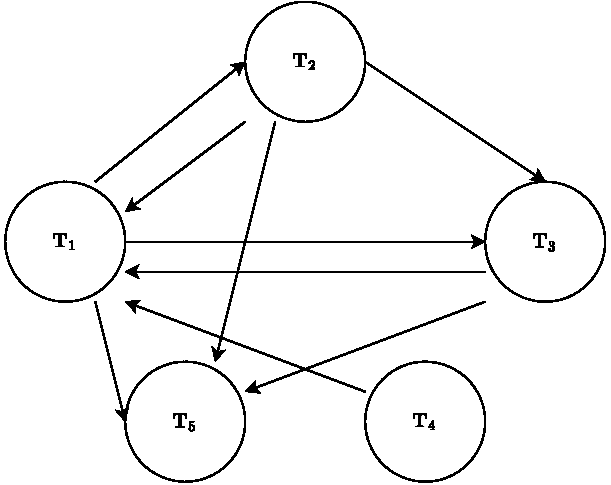
\includegraphics[width=.7\textwidth]{img/CSR-2.pdf}
	\end{figure}
	
	\noindent
	Il grafo non è aciclico, quindi $S_{3}$ non è CSR, quindi si verifica se può essere VSR. Si inizia calcolando l'insieme LeggeDa e ScrittureFinali:
	\begin{equation*}
		\begin{array}{lll}
			\text{LeggeDa}\left(S_{3}\right) &=& \left\{ \left(r_{3}\left(x\right) \: w_{2}\left(x\right)\right), \left(r_{5}\left(z\right) \: w_{1}\left(z\right)\right)\right\} \\
			\text{ScrittureFinali}\left(S_{3}\right) &=& \left\{w_{5}\left(x\right), w_{1}\left(z\right), w_{5}\left(y\right)\right\}
		\end{array}
	\end{equation*}
	Adesso si cerca almeno una combinazione tra le 5 transizioni, tale per cui una di esse sia view-equivalente a $S_{3}$. Con una considerazione rapida è possibile già ottenere il risultato finale. Guardando l'insieme delle ScrittureFinali, è possibile vedere che la $5^{a}$ transizione dovrebbe avere tra la scrittura sulla risorsa $x$ e tra la scrittura sulla risorsa $y$, la scrittura sulla risorsa $z$. Questo non è possibile poiché quest'ultima appartiene alla transazione 1. Per cui, è già possibile affermare che nessuna combinazione tra le 5 transazioni, può dare una combinazione view-equivalente a $S_{3}$. Si conclude che $S_{3}$ non è VSR e quindi è NonSR.
	
	\subsubsection{Schedule 4}
	
	Dato il seguente schedule:
	\begin{equation*}
		S_{4} = r_{1}\left(x\right) \: r_{3}\left(y\right) \: w_{1}\left(y\right) \: w_{4}\left(x\right) \: w_{1}\left(t\right) \: w_{5}\left(x\right) \: r_{2}\left(z\right) \: r_{3}\left(z\right) \: w_{2}\left(z\right) \: w_{5}\left(z\right) \: r_{4}\left(t\right) \: r_{5}\left(t\right)
	\end{equation*}
	Le transazioni sono:
	\begin{equation*}
		\begin{array}{lll}
			T_{1} &:& r_{1}\left(x\right) \: w_{1}\left(y\right) \: w_{1}\left(t\right) \\
			T_{2} &:& r_{2}\left(z\right) \: w_{2}\left(z\right) \\
			T_{3} &:& r_{3}\left(y\right) \: r_{3}\left(z\right) \\
			T_{4} &:& w_{4}\left(x\right) \: r_{4}\left(t\right) \\
			T_{5} &:& w_{5}\left(x\right) \: w_{5}\left(z\right) \: r_{5}\left(t\right)
		\end{array}
	\end{equation*}
	Si verifica CSR prima di tutto. Quindi, si inizia costruendo l'insieme dei conflitti:
	\begin{enumerate}
		\item $\textcolor{Red3}{\boldsymbol{r_{1}\left(x\right)} \: }r_{3}\left(y\right) \: w_{1}\left(y\right) \: \textcolor{Red3}{\boldsymbol{w_{4}\left(x\right)} \: }w_{1}\left(t\right) \: w_{5}\left(x\right) \: r_{2}\left(z\right) \: r_{3}\left(z\right) \: w_{2}\left(z\right) \: w_{5}\left(z\right) \: r_{4}\left(t\right) \: r_{5}\left(t\right)$
		
		\item $\textcolor{Red3}{\boldsymbol{r_{1}\left(x\right)} \: }r_{3}\left(y\right) \: w_{1}\left(y\right) \: w_{4}\left(x\right) \: w_{1}\left(t\right) \: \textcolor{Red3}{\boldsymbol{w_{5}\left(x\right)} \: }r_{2}\left(z\right) \: r_{3}\left(z\right) \: w_{2}\left(z\right) \: w_{5}\left(z\right) \: r_{4}\left(t\right) \: r_{5}\left(t\right)$
		
		\item $r_{1}\left(x\right) \: \textcolor{Red3}{\boldsymbol{r_{3}\left(y\right)} \: }\textcolor{Red3}{\boldsymbol{w_{1}\left(y\right)} \: }w_{4}\left(x\right) \: w_{1}\left(t\right) \: w_{5}\left(x\right) \: r_{2}\left(z\right) \: r_{3}\left(z\right) \: w_{2}\left(z\right) \: w_{5}\left(z\right) \: r_{4}\left(t\right) \: r_{5}\left(t\right)$
		
		\item $r_{1}\left(x\right) \: r_{3}\left(y\right) \: w_{1}\left(y\right) \: \textcolor{Red3}{\boldsymbol{w_{4}\left(x\right)} \: }w_{1}\left(t\right) \: \textcolor{Red3}{\boldsymbol{w_{5}\left(x\right)} \: }r_{2}\left(z\right) \: r_{3}\left(z\right) \: w_{2}\left(z\right) \: w_{5}\left(z\right) \: r_{4}\left(t\right) \: r_{5}\left(t\right)$
		
		\item $r_{1}\left(x\right) \: r_{3}\left(y\right) \: w_{1}\left(y\right) \: w_{4}\left(x\right) \: \textcolor{Red3}{\boldsymbol{w_{1}\left(t\right)} \: }w_{5}\left(x\right) \: r_{2}\left(z\right) \: r_{3}\left(z\right) \: w_{2}\left(z\right) \: w_{5}\left(z\right) \: \textcolor{Red3}{\boldsymbol{r_{4}\left(t\right)} \: }r_{5}\left(t\right)$
		
		\item $r_{1}\left(x\right) \: r_{3}\left(y\right) \: w_{1}\left(y\right) \: w_{4}\left(x\right) \: \textcolor{Red3}{\boldsymbol{w_{1}\left(t\right)} \: }w_{5}\left(x\right) \: r_{2}\left(z\right) \: r_{3}\left(z\right) \: w_{2}\left(z\right) \: w_{5}\left(z\right) \: r_{4}\left(t\right) \: \textcolor{Red3}{\boldsymbol{r_{5}\left(t\right)}}$
		
		\item $r_{1}\left(x\right) \: r_{3}\left(y\right) \: w_{1}\left(y\right) \: w_{4}\left(x\right) \: w_{1}\left(t\right) \: w_{5}\left(x\right) \: \textcolor{Red3}{\boldsymbol{r_{2}\left(z\right)} \: }r_{3}\left(z\right) \: w_{2}\left(z\right) \: \textcolor{Red3}{\boldsymbol{w_{5}\left(z\right)} \: }r_{4}\left(t\right) \: r_{5}\left(t\right)$
		
		\item $r_{1}\left(x\right) \: r_{3}\left(y\right) \: w_{1}\left(y\right) \: w_{4}\left(x\right) \: w_{1}\left(t\right) \: w_{5}\left(x\right) \: r_{2}\left(z\right) \: \textcolor{Red3}{\boldsymbol{r_{3}\left(z\right)} \: }\textcolor{Red3}{\boldsymbol{w_{2}\left(z\right)} \: }w_{5}\left(z\right) \: r_{4}\left(t\right) \: r_{5}\left(t\right)$
		
		\item $r_{1}\left(x\right) \: r_{3}\left(y\right) \: w_{1}\left(y\right) \: w_{4}\left(x\right) \: w_{1}\left(t\right) \: w_{5}\left(x\right) \: r_{2}\left(z\right) \: \textcolor{Red3}{\boldsymbol{r_{3}\left(z\right)} \: }w_{2}\left(z\right) \: \textcolor{Red3}{\boldsymbol{w_{5}\left(z\right)} \: }r_{4}\left(t\right) \: r_{5}\left(t\right)$
		
		\item $r_{1}\left(x\right) \: r_{3}\left(y\right) \: w_{1}\left(y\right) \: w_{4}\left(x\right) \: w_{1}\left(t\right) \: w_{5}\left(x\right) \: r_{2}\left(z\right) \: r_{3}\left(z\right) \: \textcolor{Red3}{\boldsymbol{w_{2}\left(z\right)} \: } \textcolor{Red3}{\boldsymbol{w_{5}\left(z\right)} \: } r_{4}\left(t\right) \: r_{5}\left(t\right)$
	\end{enumerate}
	Quindi, l'insieme dei conflitti è:
	\begin{equation*}
		\begin{array}{lll}
			\text{Conflitti}\left(S_{4}\right) = \{ & \left(r_{1}\left(x\right) \: w_{4}\left(x\right)\right), \left(r_{1}\left(x\right) \: w_{5}\left(x\right)\right), & \\ [0.5em]
													& \left(r_{3}\left(y\right) \: w_{1}\left(y\right)\right), & \\ [0.5em]
													& \left(w_{4}\left(x\right) \: w_{5}\left(x\right)\right), & \\ [0.5em]
													& \left(w_{1}\left(t\right) \: r_{4}\left(t\right)\right), \left(w_{1}\left(t\right) \: r_{5}\left(t\right)\right) & \\ [0.5em]
													& \left(r_{2}\left(z\right) \: w_{5}\left(z\right)\right), & \\ [0.5em]
													& \left(r_{3}\left(z\right) \: w_{2}\left(z\right)\right), \left(r_{3}\left(z\right) \: w_{5}\left(z\right)\right), & \\ [0.5em]
													& \left(w_{2}\left(z\right) \: w_{5}\left(z\right)\right) & \}
		\end{array}
	\end{equation*}\newpage

	\noindent
	Adesso si costruisce il grafo. I nodi sono 5 poiché il numero di transazioni è 5:
	\begin{figure}[!htp]
		\centering
		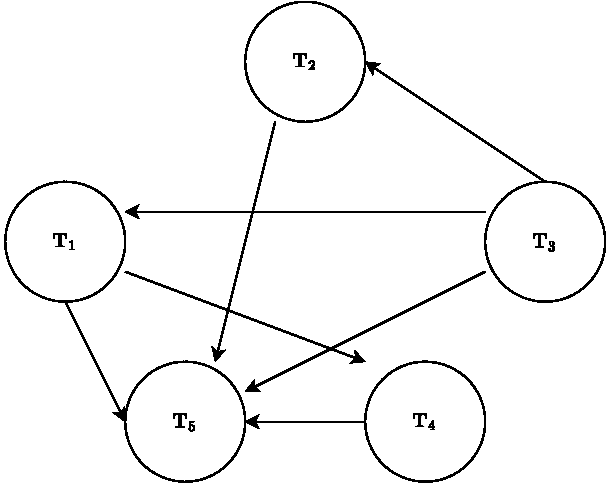
\includegraphics[width=.7\textwidth]{img/CSR-3.pdf}
	\end{figure}

	\noindent
	Il grafo risulta aciclico, quindi è possibile affermare con certezza che $S_{4}$ è CSR e per definizione anche VSR ($CSR \subset VSR$). Per concludere l'esercizio, è necessario calcolare gli schedule seriali equivalenti. Per capire quali combinazioni sono accettate, si fanno alcune considerazioni guardando il grafo:
	\begin{itemize}
		\item Il nodo $T_{5}$ non ha archi orientati in uscita, ma solo in entrata. Quindi, è possibile affermare che la transazione $T_{5}$ deve essere l'ultima.
		
		\item Il nodo $T_{3}$ non ha archi orientati in entrata, ma solo in uscita. Quindi, è possibile affermare che la transazione $T_{3}$ deve essere la prima.
		
		\item I nodi $T_{2}$ e $T_{1}$ sono gli unici che vengono raggiunti da $T_{3}$, ovvero dal nodo d'inizio. Quindi, è possibile affermare che le uniche combinazioni potranno essere:
		\begin{enumerate}
			\item $T_{3}, T_{1}, T_{2}, T_{4}, T_{5}$
			\item $T_{3}, T_{1}, T_{4}, T_{2}, T_{5}$
			\item $T_{3}, T_{2}, T_{1}, T_{4}, T_{5}$
			\item $T_{3}, T_{2}, T_{4}, T_{1}, T_{5}$
		\end{enumerate}

		\item Dal nodo $T_{1}$ è possibile andare al nodo $T_{4}$ senza problemi ma non viceversa poiché altrimenti si creerebbe una ciclo. Quindi le uniche combinazioni ammesse sono:
		\begin{enumerate}
			\item $T_{3}, T_{1}, T_{2}, T_{4}, T_{5}$
			\item $T_{3}, T_{1}, T_{4}, T_{2}, T_{5}$
			\item $T_{3}, T_{2}, T_{1}, T_{4}, T_{5}$
			\item $T_{3}, T_{2}, T_{4}, T_{1}, T_{5}$
		\end{enumerate}
	\end{itemize}\newpage
	
	\subsection{Ottimizzazione e stima di costo}
	
	\subsubsection{Esercizio 1}
	
	Si consideri il seguente schema relazionale contenete le ricette di una catena di ristoranti:
	\begin{equation*}
		\begin{array}{rl}
			\textsf{INGREDIENTE} & \left(\underline{\text{Codice}}, \text{Nome}, \text{Calorie}\right); \\[0.3em]
			\textsf{COMPOSIZIONE} & \left(\underline{\text{Ricetta, Ingrediente}}, \text{Quantità}\right); \\[0.3em]
			\textsf{RICETTA} & \left(\underline{\text{CodiceRicetta}}, \text{Nome}, \text{Regione}, \text{TempoPreparazione}\right).
		\end{array}
	\end{equation*}
	N.B.: la quantità della tabella \textsf{COMPOSIZIONE} è espressa in grammi.\newline
	
	\noindent
	\emph{\textbf{Vincoli di integrità referenziale:}}
	\begin{equation*}
		\begin{array}{lll}
			\textsf{COMPOSIZIONE}.\text{Ricetta} 		&\rightarrow& \textsf{RICETTA} \\ [0.3em]
			\textsf{COMPOSIZIONE}.\text{Ingrediente} 	&\rightarrow& \textsf{INGREDIENTE}
		\end{array}
	\end{equation*}
	Data la seguente interrogazione SQL che consente di: \emph{trovare gli ingredienti usati in ricette della Regione Veneto, riportando, il codice della ricetta e il nome e le calorie dell'ingrediente}.
	\lstinputlisting[language=SQL]{code/ottimizzazione-1.sql}
	Calcolare il costo dell'interrogazione in termini di numero di accessi a memoria secondaria sotto le seguenti ipotesi:
	\begin{itemize}
		\item La selezione su ricetta richiede una scansione sequenziale della tabella \textsf{RICETTA};
		
		\item L'ordine di esecuzione del join è:
		\begin{equation*}
			\left(\textsf{RICETTA} \Join \textsf{COMPOSIZIONE}\right) \Join \textsf{INGREDIENTE}
		\end{equation*}
		
		\item Le operazioni di join vengono eseguite con la tecnica \underline{Nested Loop join} con una pagina di buffer disponibile per ogni tabella;
		
		\item Il risultato intermedio del primo join viene interamente memorizzato nel buffer;
		
		\item $\mathrm{NP}\left(\textsf{INGREDIENTE}\right) = 40$, $\mathrm{NP}\left(\textsf{COMPOSIZIONE}\right) = 200$, $\mathrm{NP}\left(\textsf{RICETTA}\right) = 12$;
		
		\item $\mathrm{NR}\left(\textsf{INGREDIENTE}\right) = 1200$, $\mathrm{NR}\left(\textsf{COMPOSIZIONE}\right) = 13000$, $\mathrm{NR}\left(\textsf{RICETTA}\right) = 260$;
		
		\item $\mathrm{VAL}\left(\text{Regione}, \textsf{RICETTA}\right) = 20$, $\mathrm{VAL}\left(\text{Ricetta}, \textsf{COMPOSIZIONE}\right) = 260$.
	\end{itemize}
	Come cambia il costo se è disponibile un indice B+-tree sull'attributo Codice della tabella INGREDIENTE che ha profondità 2.\newpage
	
	\noindent
	Il \emph{nested loop join} è un algoritmo di join che unisce due set usando due cicli nidificati. Quindi, i cicli sono:
	\begin{enumerate}
		\item Viene selezionata la regione Veneta (\textsf{WHERE R.Regione = 'Veneto'}) e successivamente eseguito il primo Join:
		\begin{equation*}
			\textsf{seleziona\_veneto}\left(\textsf{RICETTA}\right) \Join \textsf{COMPOSIZIONE}
		\end{equation*}
		Quindi il costo risulta essere una lettura della tabella esterna \textsf{RICETTA} poiché deve essere applicato una condizione \textsf{WHERE} e infine viene eseguita una moltiplicazione:
		\begin{equation*}
			\begin{array}{lll}
				\text{Costo} = & \text{NP}\left(\textsf{RICETTA}\right) + & \\
				& \mathrm{NR}\left(\textsf{RICETTA} \text{ con selezione Regione='Veneto'}\right) \times & \\
				& \mathrm{NP}\left(\textsf{COMPOSIZIONE}\right)
			\end{array}
		\end{equation*}
		
		\item Il secondo Join non prevede condizioni \textsf{WHERE} e il costo non tiene in considerazione una lettura da una tabella esterna poiché la tabella interessata è già in buffer:
		\begin{equation*}
			\begin{array}{lll}
				\text{Costo} = & \mathrm{NR}\left(\textsf{COMPOSIZIONE} \text{ per le ricette con selezione Regione='Veneto'}\right) \times & \\
				& \mathrm{NP}\left(\textsf{INGREDIENTE}\right)
			\end{array}
		\end{equation*}
	\end{enumerate}
	I dati dell'esercizio sui costi sono i seguenti:
	\begin{table}[!htp]
		\centering
		\begin{tabular}{@{} l | c c c c @{}}
			\toprule
			Tabella & NP & NR & VAL(Regione) & VAL(Ricetta) \\
			\midrule
			\textsf{Ricetta} 		& 12 & 260 & 20 & \ding{55} \\
			\textsf{Ingrediente}	& 40 & 1200 & \ding{55} & \ding{55} \\
			\textsf{Composizione}	& 200 & 13000 & \ding{55} & 260 \\
			\bottomrule
		\end{tabular}
	\end{table}
	
	\noindent
	I dati presi sono stati acquisiti dai requisiti elencati, niente di difficile. Adesso si cerca di ottenere un valore tangibile, quindi si sostituiscono i valori:
	\begin{equation*}
		\text{Costo} = 12 + \mathrm{NR}\left(\textsf{RICETTA}\right) \div \mathrm{VAL}\left(\text{Regione}, \textsf{RICETTA}\right) \times 200
	\end{equation*}
	La selezione della regione Veneto sulla tabella \textsf{RICETTA} è eseguita con la condizione:
	\begin{equation*}
		\mathrm{NR}\left(\textsf{RICETTA}\right) \div \mathrm{VAL}\left(\text{Regione}, \textsf{RICETTA}\right)
	\end{equation*}
	Andando a sostituire nuovamente i dati:
	\begin{equation*}
		\text{Costo} = 12 + 260 \div 20 \times 200 = 2'612
	\end{equation*}\newpage
	
	\noindent
	Il costo del secondo Join è possibile calcolarlo allo stesso modo. 
	\begin{equation*}
		\text{Costo} = \mathrm{NR}\left(\textsf{COMPOSIZIONE}\right) \div \mathrm{VAL}\left(\text{Ricetta}, \textsf{COMPOSIZIONE}\right) \times 13 \times 40
	\end{equation*}
	\begin{itemize}
		\item $\mathrm{NR}\left(\textsf{COMPOSIZIONE}\right) \div \mathrm{VAL}\left(\text{Ricetta}, \textsf{COMPOSIZIONE}\right)$, rappresenta il calcolo da eseguire poiché nella tabella \textsf{COMPOSIZIONE} la Ricetta è una chiave esterna;
		
		\item $13$, il valore ottenuto dal costo precedente, ovvero rappresenta il numero di regioni del veneto sulla tabella \textsf{RICETTA};
		
		\item $40$, rappresenta $\mathrm{NP}\left(\textsf{INGREDIENTE}\right)$, come da formula.
	\end{itemize}
	Quindi, il costo totale del secondo Join:
	\begin{equation*}
		\text{Costo} = 13'000 \div 260 \times 13 \times 40 = 26'000
	\end{equation*}
	E infine, il costo totale delle operazioni:
	\begin{equation*}
		\text{Costo totale} = 2'612 + 26'000 = 28'612
	\end{equation*}
	Qua di seguito, viene riportato il costo totale nel caso in cui sia disponibile un indice B+-tree sull'attributo Codice della tabella \textsf{INGREDIENTE} che ha profondità 2. Il costo sul primo Join non viene influenzato poiché non riguarda la tabella \textsf{INGREDIENTE} e quindi rimane uguale a $2'612$. Invece, il secondo Join viene influenzato poiché al posto di utilizzare NP(\textsf{INGREDIENTE}), si utilizza la profondità dell'albero, ovvero:
	\begin{equation*}
		\text{Costo secondo Join} = \left(13'000 \div 260\right) \times 13 \times \left(2+1\right) = 650 \times 3 = 1'950
	\end{equation*}
	E quindi il costo totale:
	\begin{equation*}
		\text{Costo totale} = 2'612 + 1'950 = 4'562
	\end{equation*}\newpage
	
	\subsubsection{Esercizio 2}
	
	Si consideri il seguente schema relazionale contenete le ricette di una catena di ristoranti:
	\begin{equation*}
		\begin{array}{rl}
			\textsf{RICETTA} & \left(\text{Nome}, \text{Descrizione}, \text{Regione}\right); \\[0.3em]
			\textsf{IN\_RICETTA} & \left(\text{Ricetta}, \text{Ingrediente}, \text{Quantità}\right); \\[0.3em]
			\textsf{INGREDIENTE} & \left(\text{Nome}, \text{Descrizione}\right).
		\end{array}
	\end{equation*}
	N.B.: la quantità della tabella \textsf{COMPOSIZIONE} è espressa in grammi.\newline
	
	\noindent
	\emph{\textbf{Vincoli di integrità referenziale:}}
	\begin{equation*}
		\begin{array}{lll}
			\textsf{IN\_RICETTA}.\text{Ricetta} 		&\rightarrow& \textsf{RICETTA} \\ [0.3em]
			\textsf{IN\_RICETTA}.\text{Ingrediente} 	&\rightarrow& \textsf{INGREDIENTE}
		\end{array}
	\end{equation*}
	Data la seguente interrogazione SQL:
	\lstinputlisting[language=SQL]{code/ottimizzazione-2.sql}
	Calcolare il costo dell'interrogazione in termini di numero di accessi a memoria secondaria sotto le seguenti ipotesi:
	\begin{itemize}
		\item La selezione sulla tabella \textsf{IN\_RICETTA} eseguita attraverso una scansione della tabella medesima, il risultato della selezione viene salvato in memoria secondaria in 180 pagine e riutilizzato per il join;
		
		\item La selezione delle ricette viene eseguita attraverso una scansione della tabella \textsf{RICETTA}, il risultato della selezione viene mantenuto nel buffer;
		
		\item L'ordine di esecuzione del join è:
		\begin{equation*}
			\textsf{RICETTA} \Join \textsf{IN\_RICETTA}
		\end{equation*}
		E le operazioni di join vengono eseguite con la tecnica \dquotes{Nested Loop Join} con una pagina di buffer disponibile per ogni tabella;
		
		\item $\mathrm{NP}\left(\textsf{INGREDIENTE}\right) = 30$, $\mathrm{NP}\left(\textsf{IN\_RICETTA}\right) = 780$, $\mathrm{NP}\left(\textsf{RICETTA}\right) = 150$;
		
		\item $\mathrm{NR}\left(\textsf{INGREDIENTE}\right) = 270$, $\mathrm{NR}\left(\textsf{IN\_RICETTA}\right) = 19'800$, $\mathrm{NR}\left(\textsf{RICETTA}\right) = 900$;
		
		\item $\mathrm{VAL}\left(\text{Regione}, \textsf{RICETTA}\right) = 18$, $\mathrm{VAL}\left(\text{Ricetta}, \textsf{IN\_RICETTA}\right) = 90$, \newline $\mathrm{VAL}\left(\text{Quantita}, \textsf{IN\_RICETTA}\right) = 50$.
	\end{itemize}
	Come cambia il costo se è disponibile un indice B+-tree sull'attributo Ricetta della tabella \textsf{IN\_RICETTA} che ha profondità 2.\newpage
	
	\noindent
	I dati dell'esercizio sui costi sono i seguenti:
	\begin{table}[!htp]
		\centering
		\begin{tabular}{@{} l | c c c c c @{}}
			\toprule
			Tabella & NP & NR & VAL(Regione) & VAL(Ricetta) & VAL(Quantita) \\
			\midrule
			\textsf{Ricetta} 		& 150 & 900 & 18 & \ding{55} & \ding{55} \\
			\textsf{In\_ricetta}	& 780 & 19800 & \ding{55} & 90 & 50 \\
			\textsf{Ingrediente}	& 30 & 270 & \ding{55} & \ding{55} & \ding{55} \\
			\bottomrule
		\end{tabular}
	\end{table}
	
	\noindent
	Come viene esplicitato dall'esercizio, la selezione sulla tabella \textsf{IN\_RICETTA} viene eseguita:
	\begin{enumerate}
		\item Facendo una scansione della tabella medesima:
		\begin{equation*}
			\mathrm{NP}\left(\textsf{IN\_RICETTA}\right) = 780
		\end{equation*}
		
		\item Il risultato della selezione viene salvato in memoria secondaria in 180 pagine, quindi:
		\begin{equation*}
			\mathrm{NP}\left(\textsf{IN\_RICETTA}\right) = 780 \Longrightarrow 180
		\end{equation*}
		
		\item Viene utilizzato il valore per il Join. Quindi, dato che non vi sono letture di tabelle poiché il buffer contiene già i valori d'interesse, il costo è:
		\begin{equation*}
			\begin{array}{lll}
				\text{Costo} &=& \mathrm{NR}\left(\textsf{RICETTA}\right) \div \mathrm{VAL}\left(\text{Regione}, \textsf{RICETTA}\right) \times \mathrm{NP}\left(\textsf{IN\_RICETTA}\right) \\
				&=& 900 \div 18 \times 180 \\
				&=& 50 \times 180 \\
				&=& 9'000
			\end{array}
		\end{equation*}
		Ricordando che si utilizzano 180 pagine e non 780 (punto 2).
	\end{enumerate}
	Quindi, il costo totale è dato, rispettivamente, dalla somma delle pagine di \textsf{IN\_RICETTA}, dalle pagine scritte nella memoria secondaria che si riferiscono a \textsf{IN\_RICETTA}, dal Join eseguito qua sopra e infine dalla scansione della tabella \textsf{RICETTA}:
	\begin{equation*}
		\text{Costo totale} = 780 + 180 + 9'000 + 150 = 10'110
	\end{equation*}
	Per quanto riguarda il caso in cui fosse presente un indice B+-tree, è necessario modificare il Join. Quindi diventa la formula:
	\begin{equation*}
		\begin{array}{lll}
			\text{Costo Join} &=& \mathrm{NR}\left(\text{\textsf{RICETTA} con selezione}\right) \div \mathrm{VAL}\left(\text{Regione}, \textsf{RICETTA}\right) \times \\
			&& \left(\text{Prof. Indice} + \mathrm{NR}\left(\textsf{IN\_RICETTA}\text{ con selezione}\right) \div \mathrm{VAL}\left(\text{q.ta}, \textsf{IN\_RICETTA}\right)\right) \\
			&=& 900 \div 18 \times \left(19'800 \div 50\right) \div 90 \\
			&=& 220
		\end{array}
	\end{equation*}
	Il totale quindi diventa:
	\begin{equation*}
		\text{Costo totale} = 780 + 180 + 150 + 220 = 1'330
	\end{equation*}\newpage
	
	\subsubsection{Esercizio 3}
	
	Si consideri il seguente schema relazionale:
	\begin{equation*}
		\begin{array}{ll}
			\textsf{COMUNE} 	& \left(\text{CodISTAT, Nome, Abitanti, Superficie, Prov, TipoTerritorio}\right) \\ [0.3em]
			\textsf{ADIACENTE} 	& \left(\text{Comune1, Comune2}\right) \\ [0.3em]
			\textsf{PROVINCIA} 	& \left(\text{Codice, NomeProv, SuperficieProv, Regione}\right) 
		\end{array}
	\end{equation*}
	Con il dato TipoTerritorio: \{montagna, mare, pianura, collina\}.\newline
	
	\noindent
	La tabella \textsf{ADIACENTE} rappresenta la relazione di adiacenza tra comuni: poiché la relazione è simmetrica per rappresentare l'adiacenza tra i comuni A e B si memorizza sia la tupla (A,B) sia la tupla (B,A).\newline
	
	\noindent
	Vincoli d'integrità:
	\begin{equation*}
		\begin{array}{rcl}
			\textsf{ADIACENTE}.\text{Comune1} &\rightarrow& \textsf{COMUNE} \\
			\textsf{ADIACENTE}.\text{Comune2} &\rightarrow& \textsf{COMUNE} \\
			\textsf{COMUNE}.\text{Prov} &\rightarrow& \textsf{PROVINCIA} 
		\end{array}
	\end{equation*}
	Dato lo schema dell'esercizio, si consideri la seguente interrogazione:
	\lstinputlisting[language=SQL]{code/ottimizzazione-3.sql}
	Indicare una stima del costo dell'interrogazione in termini di numero di accessi a memoria secondaria  sapendo che: (i) la selezione dei comuni viene eseguita attraverso una scansione della tabella \textsf{COMUNE} e il risultato viene mantenuto nel buffer:
	\begin{itemize}
		\item L'ordine di esecuzione del join è:
		\begin{equation*}
			\textsf{COMUNE} \Join \textsf{ADIACENTE}
		\end{equation*}
		E viene applicata la tecnica \dquotes{Nested Loop Join} e con indice B+-tree di profondità 3 sull'attributo Comune1 della tabella \textsf{ADIACENTE};
		
		\item I dati sono:
		\begin{equation*}
			\begin{array}{rll}
				\mathrm{NP}\left(\textsf{COMUNE}\right) &=& 15; \\
				\mathrm{NR}\left(\textsf{COMUNE}\right) &=& 1'900; \\
				\mathrm{NP}\left(\textsf{ADIACENTE}\right) &=& 155; \\
				\mathrm{NR}\left(\textsf{ADIACENTE}\right) &=& 38'000; \\
				\mathrm{VAL}\left(\text{TipoTerritorio}, \textsf{COMUNE}\right) &=& 4; \\
				\mathrm{VAL}\left(\text{Comune1}, \textsf{ADIACENTE}\right) &=& 1'900;
			\end{array}
		\end{equation*}
	\end{itemize}\newpage
	
	\noindent
	I dati messi a disposizione sono i seguenti:
	\begin{table}[!htp]
		\centering
		\begin{tabular}{@{} l | c c c c @{}}
			\toprule
			Tabella & NP & NR & VAL(TipoTerritorio) & VAL(Comune1) \\
			\midrule
			\textsf{COMUNE}		& 15		& 1'900		& 4			& \ding{55} \\
			\textsf{ADIACENTE}	& 155		& 38'000	& \ding{55} & 1'900		\\
			\textsf{PROVINCIA}	& \ding{55}	& \ding{55}	& \ding{55} & \ding{55} \\
			\bottomrule
		\end{tabular}
	\end{table}
	
	\noindent
	Viene richiesto il costo per:
	\begin{itemize}
		\item Eseguire una scansione della tabella \textsf{COMUNE} poiché viene eseguita una selezione dei comuni. Questo risultato è semplice poiché corrisponde a:
		\begin{equation*}
			\text{Costo} = \text{scrittura} + \text{lettura} = \mathrm{NP}\left(\textsf{COMUNE}\right) + 0 = 15
		\end{equation*}
		
		\item Eseguire il Join con la tecnica \dquotes{Nested Loop Join} senza albero B+-tree. Quindi, viene calcolato nel seguente modo il costo:
		\begin{equation*}
			\text{Costo} = 0 + \mathrm{NR}\left(\textsf{COMUNE}\right) \div \mathrm{VAL}\left(\text{TipoTerritorio}, \textsf{COMUNE}\right) \times \mathrm{NP}\left(\textsf{ADIACENTE}\right)
		\end{equation*}
		Il valore zero indica che nel buffer non viene eseguita nessuna scrittura poiché è già stata fatta in precedenza (punto precedente). Quindi, andando a sostituire i valori:
		\begin{equation*}
			\text{Costo} = 0 + 1'900 \div 4 \times 155 = 475 \times 155 = 73'625
		\end{equation*}
		
		\item Eseguire il Join con la tecnica \dquotes{Nested Loop Join} con albero B+-tree di profondità 3 sull'attributo Comune1. Quindi, viene calcolato nel seguente modo il costo:
		\begin{equation*}
			\begin{array}{lll}
				\text{Costo} &=& 0 + \mathrm{NR}\left(\textsf{COMUNE}\right) \div \mathrm{VAL}\left(\text{TipoTerritorio}, \textsf{COMUNE}\right) \times \\
				&& \left(\text{Profondità Indice } + \mathrm{NR}\left(\textsf{ADIACENTE}\right) \div \mathrm{VAL}\left(\text{Comune1}, \textsf{ADIACENTE}\right)\right) \\
				&=& 0 + 1'900 \div 4 \times \left(3 + 38'000 \div 1'900\right) \\
				&=& 475 \times 23 \\
				&=& 10'925
			\end{array}
		\end{equation*}
	\end{itemize}
	
	\newpage
	
	\subsection{XML}
	
	\subsubsection{Esercizio 1}
	
	Dato il seguente frammento XML:
	\lstinputlisting[language=XML]{code/xml-1.xml}
	\begin{itemize}
		\item Generare il corrisponde XSD, supponendo che ogni conto abbia uno o più clienti intestatari.
		
		\item Modificare la struttura dell'XML per ridurre la ridondanza e rappresentare una sola volta gli elementi ripetuti.
	\end{itemize}\newpage
	
	\noindent
	\textcolor{Green4}{\underline{\textbf{\emph{Soluzione pt.1}}}}\newline
	
	\noindent
	Qua di seguito il codice soluzione dell'esercizio supponendo che ogni conto abbia uno o più intestatari:
	\lstinputlisting[language=XML]{code/xml-3.xsd}\newpage
	
	\noindent
	\textcolor{Green4}{\underline{\textbf{\emph{Soluzione pt.2}}}}\newline
	
	\noindent
	Qua di seguito il codice soluzione dell'esercizio supponendo che ogni conto abbia uno o più intestatari:
	\lstinputlisting[language=XML]{code/xml-4.xsd}
	A seguito delle modifiche di questo schema, l'istanza del documento diventa:
	\lstinputlisting[language=XML]{code/xml-5.xml}\newpage
	
	\subsubsection{Esercizio 2}
	Dato il seguente documento XML, produrre una specifica XML schema alla quale tale documento sia conforme:
	\lstinputlisting[language=XML]{code/xml-2.xml}
	I requisiti sono i seguenti. Il tipo può assumere solo uno dei seguenti valori: \{privato, attivita commerciale, attivita professionale, servizio pubblico\}. L'attributo \textsf{id} è obbligatorio. Supponiamo per semplicità che il civico sia sempre un intero positivo. Si desuma il tipo per il numero di telefono dalle istanze nel documento XML.\newpage
	
	\noindent
	\textcolor{Green4}{\underline{\textbf{\emph{Soluzione}}}}
	\lstinputlisting[language=XML]{code/xml-6.xsd}\newpage

	\section{Domande di teoria - Terzo parziale}
	
	Domande di teoria tratte dalla terza prova intermedia dell'esame 06/2015.
	\begin{enumerate}
		\item \textbf{(\emph{3 punti})} \textcolor{Green4}{\textbf{\emph{Illustrare l'architettura di un DBMS descrivendo in particolare il modulo di gestione dei buffer; si indichi inoltre, per ogni modulo dell'architettura, quali sono le proprietà delle transazioni che contribuisce a garantire.}}}\label{dom: gestione del buffer}
		
		L'architettura di un DBMS è strutturata su 3 livelli differenti:
		\begin{itemize}
			\item Le viste, che appartengono allo schema esterno;
			\item Il modello relazionale, che appartiene allo schema logico;
			\item Le strutture fisiche, che appartengono allo schema interno.
		\end{itemize}
		Lo schema logico comunica con lo schema esterno attraverso l'indipendenza logica e con lo schema interno attraverso l'indipendenza fisica.
		\begin{figure}[!htp]
			\centering
			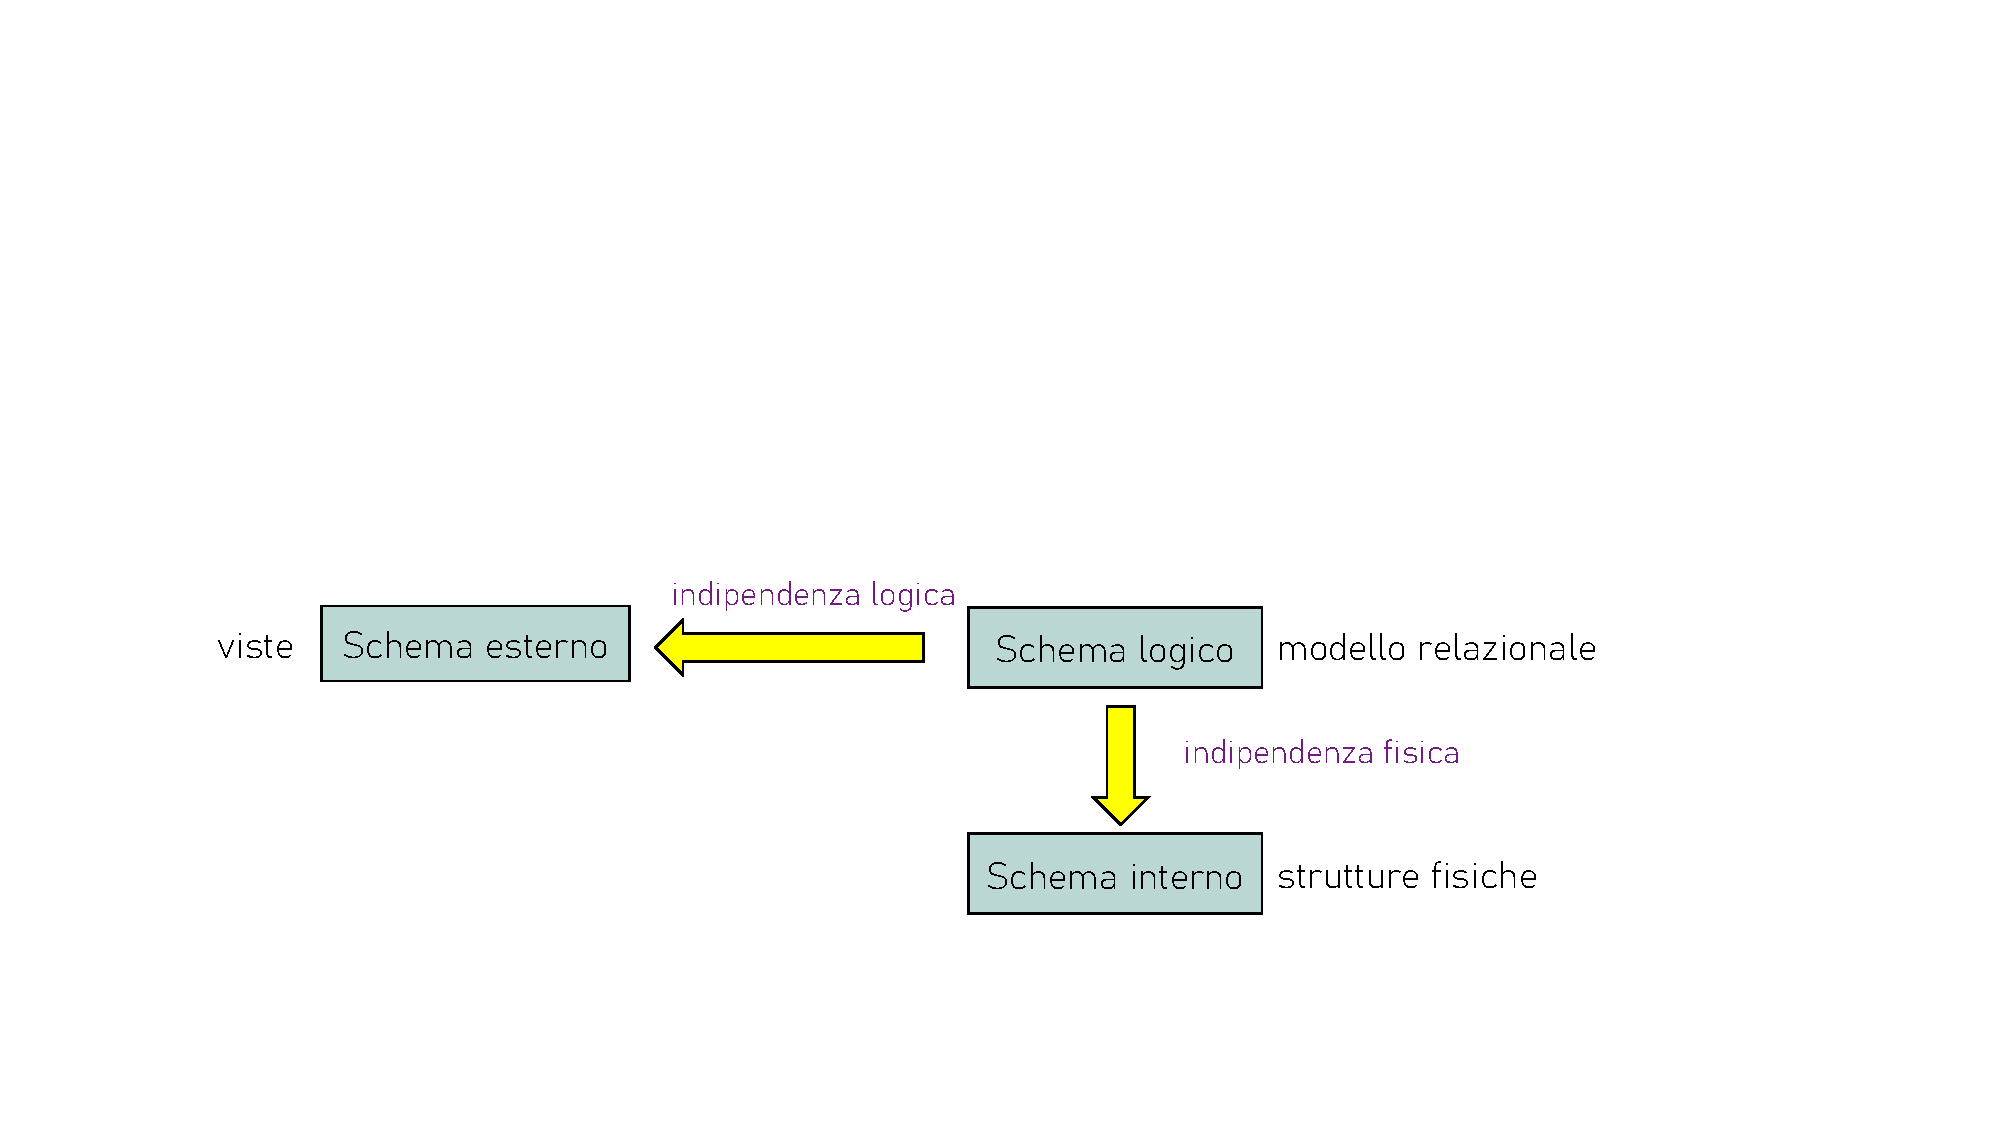
\includegraphics[width=\textwidth]{img/ex/arch-dbms-1.pdf}
		\end{figure}
		
		\noindent
		All'interno dello schema logico ci sono molteplici moduli, i quali garantiscono anche alcune proprietà delle transazioni:
		\begin{itemize}
			\item Gestore delle \textbf{interrogazioni};
			
			\item Gestore dell'\textbf{esecuzione concorrente}, il quale garantisce le proprietà di \underline{atomicità} e \underline{isolamento};
			
			\item Gestore dei \textbf{metodi d'accesso}, il quale garantisce la proprietà di \underline{consistenza};
			
			\item Gestore dell'\textbf{affidabilità}, il quale garantisce \underline{atomicità} e \underline{persistenza};
			
			\item Gestore del \textbf{buffer};
			
			\item Gestore della \textbf{memoria secondaria}.
		\end{itemize}
		Ricapitolando:
		\begin{table}[!htp]
			\centering
			\begin{tabular}{@{} l p{18em} @{}}
				\toprule
				Proprietà & Garantita da \\
				\midrule
				\textbf{Atomicità} 	& Gestore dell'\textbf{esecuzione concorrente} \newline Gestore dell'\textbf{affidabilità} \\ [0.5em]
				\textbf{Consistenza}	& Gestore dei \textbf{metodi d'accesso} \\ [0.5em]
				\textbf{Isolamento} 	& Gestore dell'\textbf{esecuzione concorrente} \\ [0.5em]
				\textbf{Persistenza} & Gestore dell'\textbf{affidabilità} \\
				\bottomrule
			\end{tabular}
		\end{table}
		\begin{figure}[!htp]
			\centering
			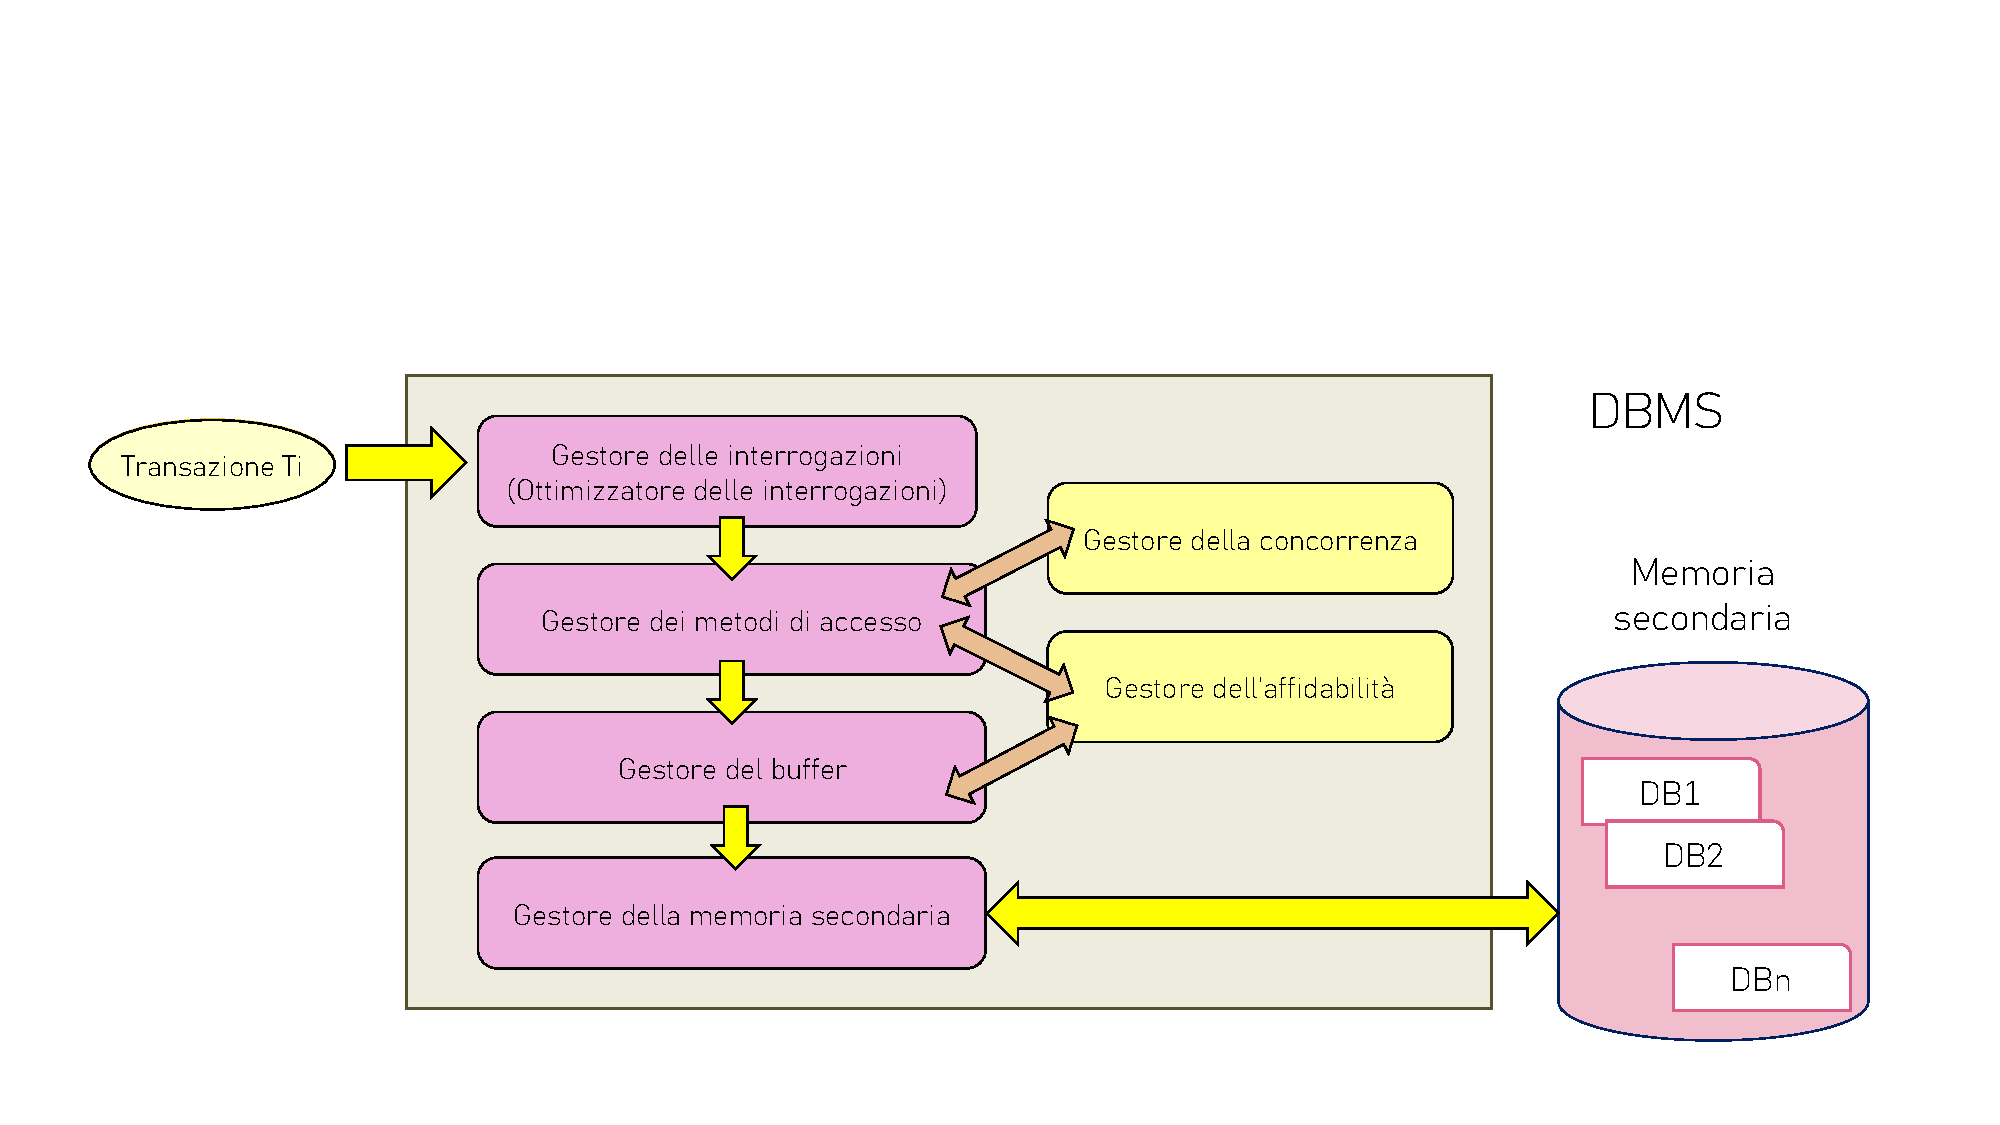
\includegraphics[width=\textwidth]{img/ex/arch-dbms-2.pdf}
		\end{figure}
		
		\noindent
		Il \textbf{modulo di gestione del buffer} è fondamentale nella \textbf{comunicazione tra memoria centrale e secondaria}. Il suo \underline{obbiettivo} è quello di \textbf{evitare accessi multipli alla memoria di massa} così da velocizzare le operazioni.\newline
		Il buffer è organizzato in pagine di dimensione pari a un numero intero di blocchi. Si occupa di caricare (lettura)/scaricare (scrittura) pagine dalle memoria centrale alla memoria di massa:
		\begin{table}[!htp]
			\centering
			\begin{tabular}{@{} l p{21em} @{}}
				\toprule
				Operazione & Descrizione \\
				\midrule
				Lettura		& Lettura dal buffer se il dato è presente, altrimenti lettura fisica dalla memoria di massa. \\ [0.5em]
				Scrittura	& Scrittura in memoria di massa se e solo se è garantita la proprietà di affidabilità del sistema, quindi se vi è la certezza che l'operazione vada a buon fine. \\
				\bottomrule
			\end{tabular}
		\end{table}
		
		\noindent
		Il modulo della gestione del buffer segue un'importante proprietà: il \textbf{principio di località dei dati}. Ovvero, \textbf{i dati referenziati di recente hanno maggior probabilità di essere referenziati nuovamente nel futuro}.\newline
		Inoltre, esiste una \textbf{legge empirica} che afferma che il 20\% dei dati è tipicamente acceduto dall'80\% delle applicazioni.
		
		Infine, il gestore del buffer memorizza le seguenti \textbf{informazioni per ogni pagina}:
		\begin{itemize}
			\item File fisico
			\item Numero di blocco
			\item (variabile di stato) Contatore, indica quanti programmi utilizzano la pagina
			\item (variabile di stato) Bit di stato, indica se la pagina è stata modificata
		\end{itemize}\newpage
		
		\begin{table}[!htp]
			\centering
			\begin{tabular}{@{} l p{23em} @{}}
				\toprule
				Concetto & Descrizione \\
				\midrule
				Architettura DBMS & L'architettura DBMS è strutturata su \textbf{3 livelli}: schema \textbf{esterno}, \textbf{logico} e \textbf{interno}. Lo schema \textbf{logico}, \textbf{il più importante}, ha al suo interno una serie di \textbf{moduli} (gestori) importanti: delle \textbf{interrogazioni}, dell'\textbf{esecuzione concorrente}, dei \textbf{metodi d'accesso}, dell'\textbf{affidabilità}, del \textbf{buffer}, della \textbf{memoria secondaria}. \\ [.7em]
				%
				Proprietà garantite & A sinistra le proprietà e a destra i moduli che le garantiscono:
				\begin{equation*}
					\begin{array}{lll}
						\textbf{Atomicità}	&\rightarrow& \text{Gestore esecuzione concorrente,} \\
											&			& \text{Gestore dell'affidabilità} \\ [.5em]
						\textbf{Consistenza}&\rightarrow& \text{Gestore dei metodi d'accesso} \\ [.5em]
						\textbf{Isolamento}	&\rightarrow& \text{Gestore esecuzione concorrente} \\ [.5em]
						\textbf{Persistenza}&\rightarrow& \text{Gestore dell'affidabilità}
					\end{array}
				\end{equation*} \\ [.7em]
				%
				Descrizione & Modulo fondamentale nella \textbf{comunicazione tra memoria centrale e di massa}, ed è \textbf{organizzato in pagine} di dimensione pari ad un numero intero di blocchi. \\ [.7em]
				%
				Obbiettivo 	& \textbf{Evitare accessi multipli alla memoria di massa} così da velocizzare le operazioni. \\ [.7em]
				%
				Cosa svolge & Esegue il \textbf{caricamento} (lettura) e \textbf{scaricamento} (scrittura) \textbf{delle pagine dalla memoria centrale alla memoria di massa}. \\ [.7em]
				%
				Principio importante & I \textbf{dati referenziati di recente} hanno maggior probabilità di essere \textbf{referenziati nuovamente nel futuro}. \\ [.7em]
				%
				Legge importante & Il \underline{20\%} dei \underline{dati} è \textbf{acceduto} dall'\underline{80\%} delle \underline{applicazioni}. \\
				\bottomrule
			\end{tabular}
			\caption{Riepilogo dei concetti della domanda sulla gestione del buffer.}
		\end{table}\newpage
		
		\item \textbf{(\emph{2 punti})} \textcolor{Green4}{\textbf{\emph{Si presenti in dettaglio la definizione di Conflict-Serializzabilità (CSR).}}}\label{dom: CSR - Conflict-Serializzabilità}
		
		Per dare la definizione di conflict-serializzabile, è necessario prima dare altre due definizioni. Due azioni eseguite da transazioni diverse, si dicono in \textbf{\underline{conflitto} se operano sullo stesso oggetto e almeno una di esse è in scrittura}. Quindi, le possibili combinazioni sono: lettura-scrittura, scrittura-lettura e scrittura-scrittura.\newline
		Uno schedule è definito \textbf{\underline{conflict-equivalente}} ad un altro schedule se \textbf{entrambi presentano le stesse operazioni e ogni coppia di operazioni in conflitto è nello stesso ordine nei due schedule}.\newline
		Adesso è possibile dare la definizione di conflict-serializzabile. Uno schedule è \textbf{\underline{conflict-serializzabile} se esiste uno schedule seriale a esso conflict-equivalente}. L'insieme degli schedule conflict-serializzabili si chiama CSR.
		
		\begin{table}[!htp]
			\centering
			\begin{tabular}{@{} l p{20em} @{}}
				\toprule
				Concetto & Descrizione \\
				\midrule
				Definizione di conflitto				& \textbf{Due azioni} di \textbf{due transazioni} \underline{diverse} sono in \textbf{conflitto} se operano sullo \textbf{stesso oggetto} e almeno una di esse è \textbf{una scrittura}. \\ [.7em]
				%
				Definizione di conflict-equivalente		& \textbf{Due schedule} sono \textbf{conflict-equivalenti} se:
				\begin{itemize}
					\item Hanno le \textbf{stesse operazioni}
					\item Ogni coppia di \textbf{operazioni in conflitto} è nello \textbf{stesso ordine} nei due schedule
				\end{itemize}\\ [.7em]
				%
				Definizione di conflict-serializzabile	& Uno schedule è conflict-serializzabile se esiste uno \textbf{schedule seriale a esso conflict-equivalente}. \\
				\bottomrule
			\end{tabular}
			\caption{Riepilogo dei concetti della domanda su CSR.}
		\end{table}\newpage
		
		\item \textbf{(\emph{2 punti})} \textcolor{Green4}{\textbf{\emph{Lo studente illustri la struttura di accesso ai dati denominata indice primario denso: caratteristiche della struttura, ricerca, inserimento e cancellazione di entry dall'indice.}}}\label{dom: indice primario denso}
		
		Un indice primario utilizza una chiave di ricerca che coincide con la chiave di ordinamento del file sequenziale. Esistono due varianti dell'indice primario, una di queste è l'\textbf{indice denso}: \textbf{per ogni occorrenza della chiave presente nel file esiste un corrispondente record nell'indice}.
		\begin{figure}[!htp]
			\centering
			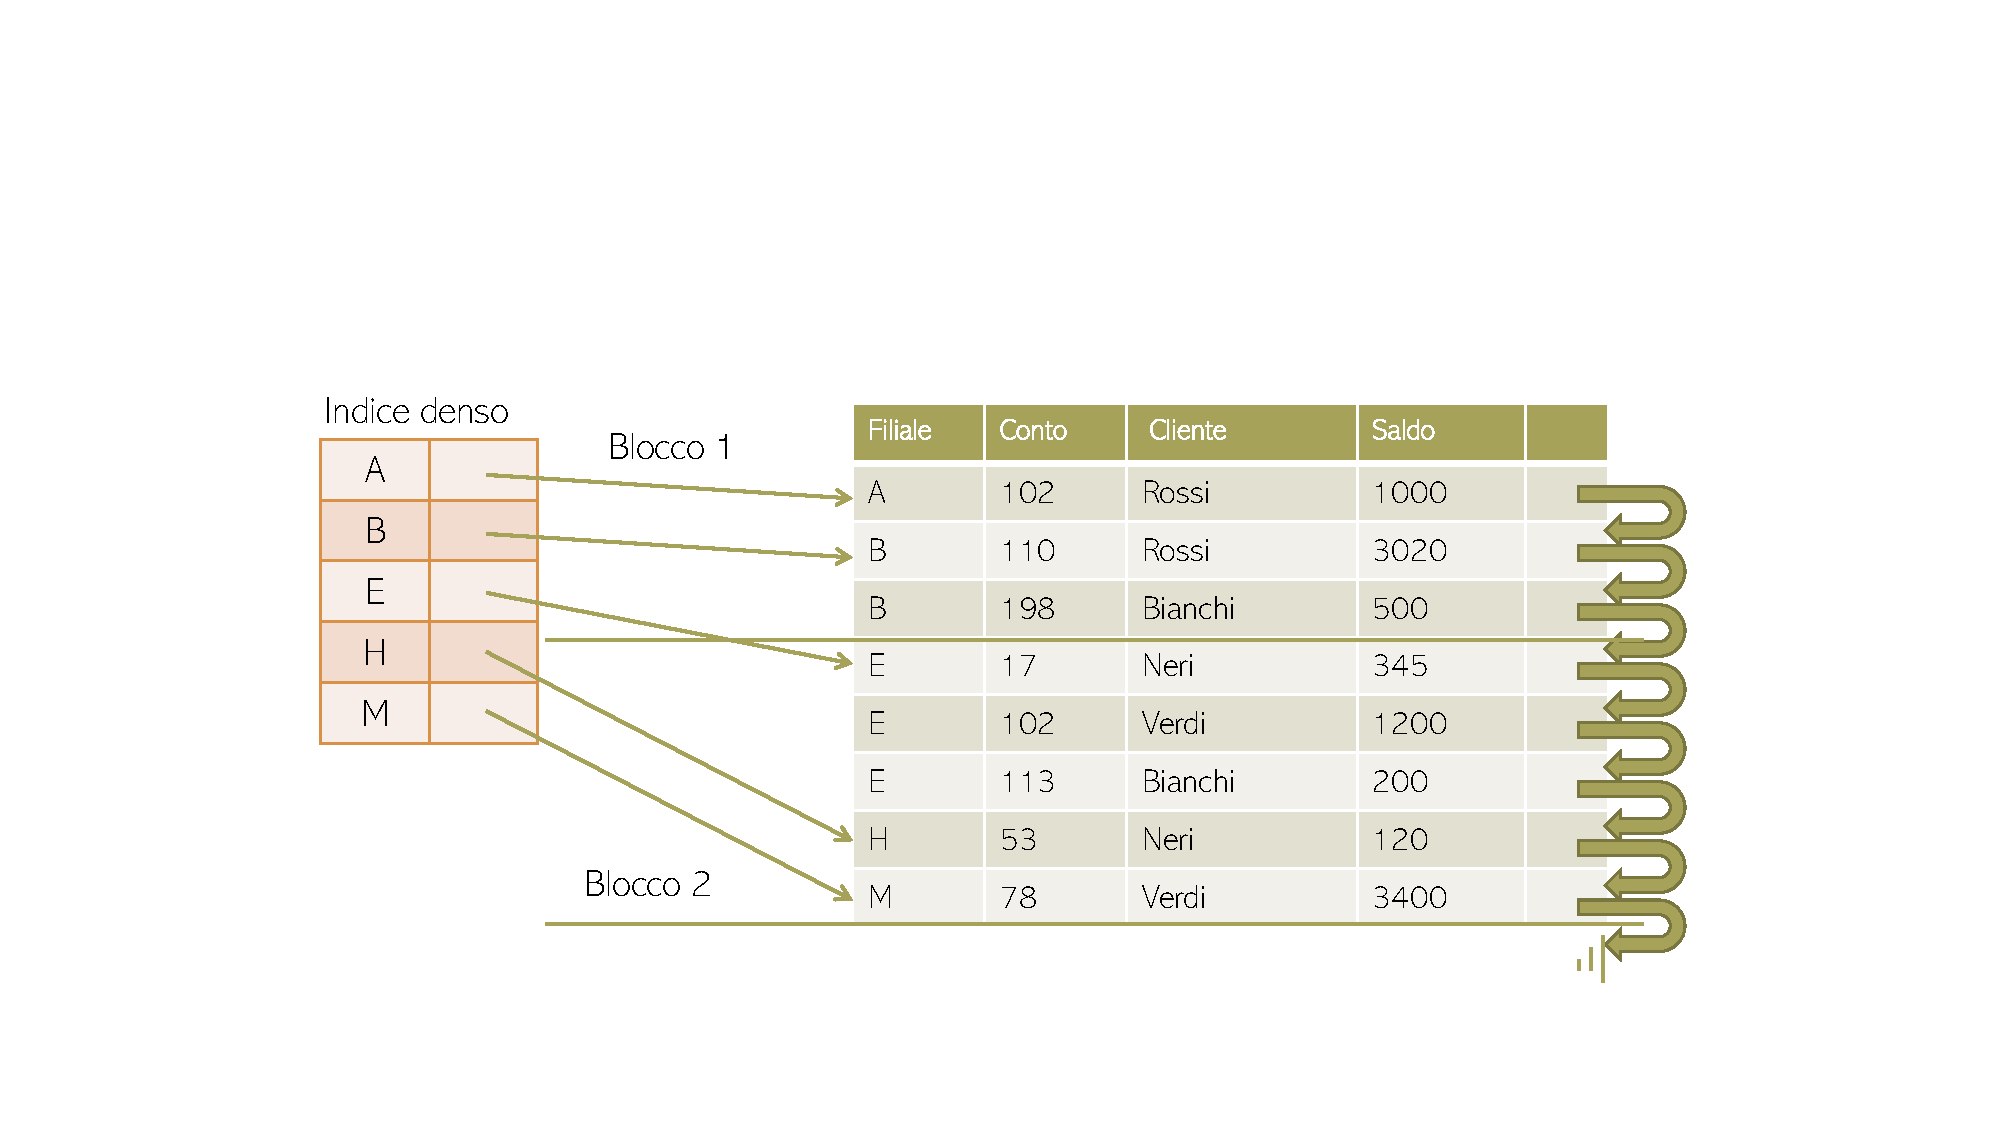
\includegraphics[width=.9\textwidth]{img/ex/indice-denso-1.pdf}
		\end{figure}
		
		\noindent
		Operazione di \textbf{ricerca}: la \textbf{ricerca avviene tramite una scansione sequenziale dell'indice per trovare il record}. Una volta trovato, viene \textbf{effettuato l'accesso al file attraverso il puntatore}. Il costo è pari a:
		\begin{equation*}
			\text{Costo} = 1 \text{ accesso indice } + 1 \text{ accesso blocco dati}
		\end{equation*}
		\begin{figure}[!htp]
			\centering
			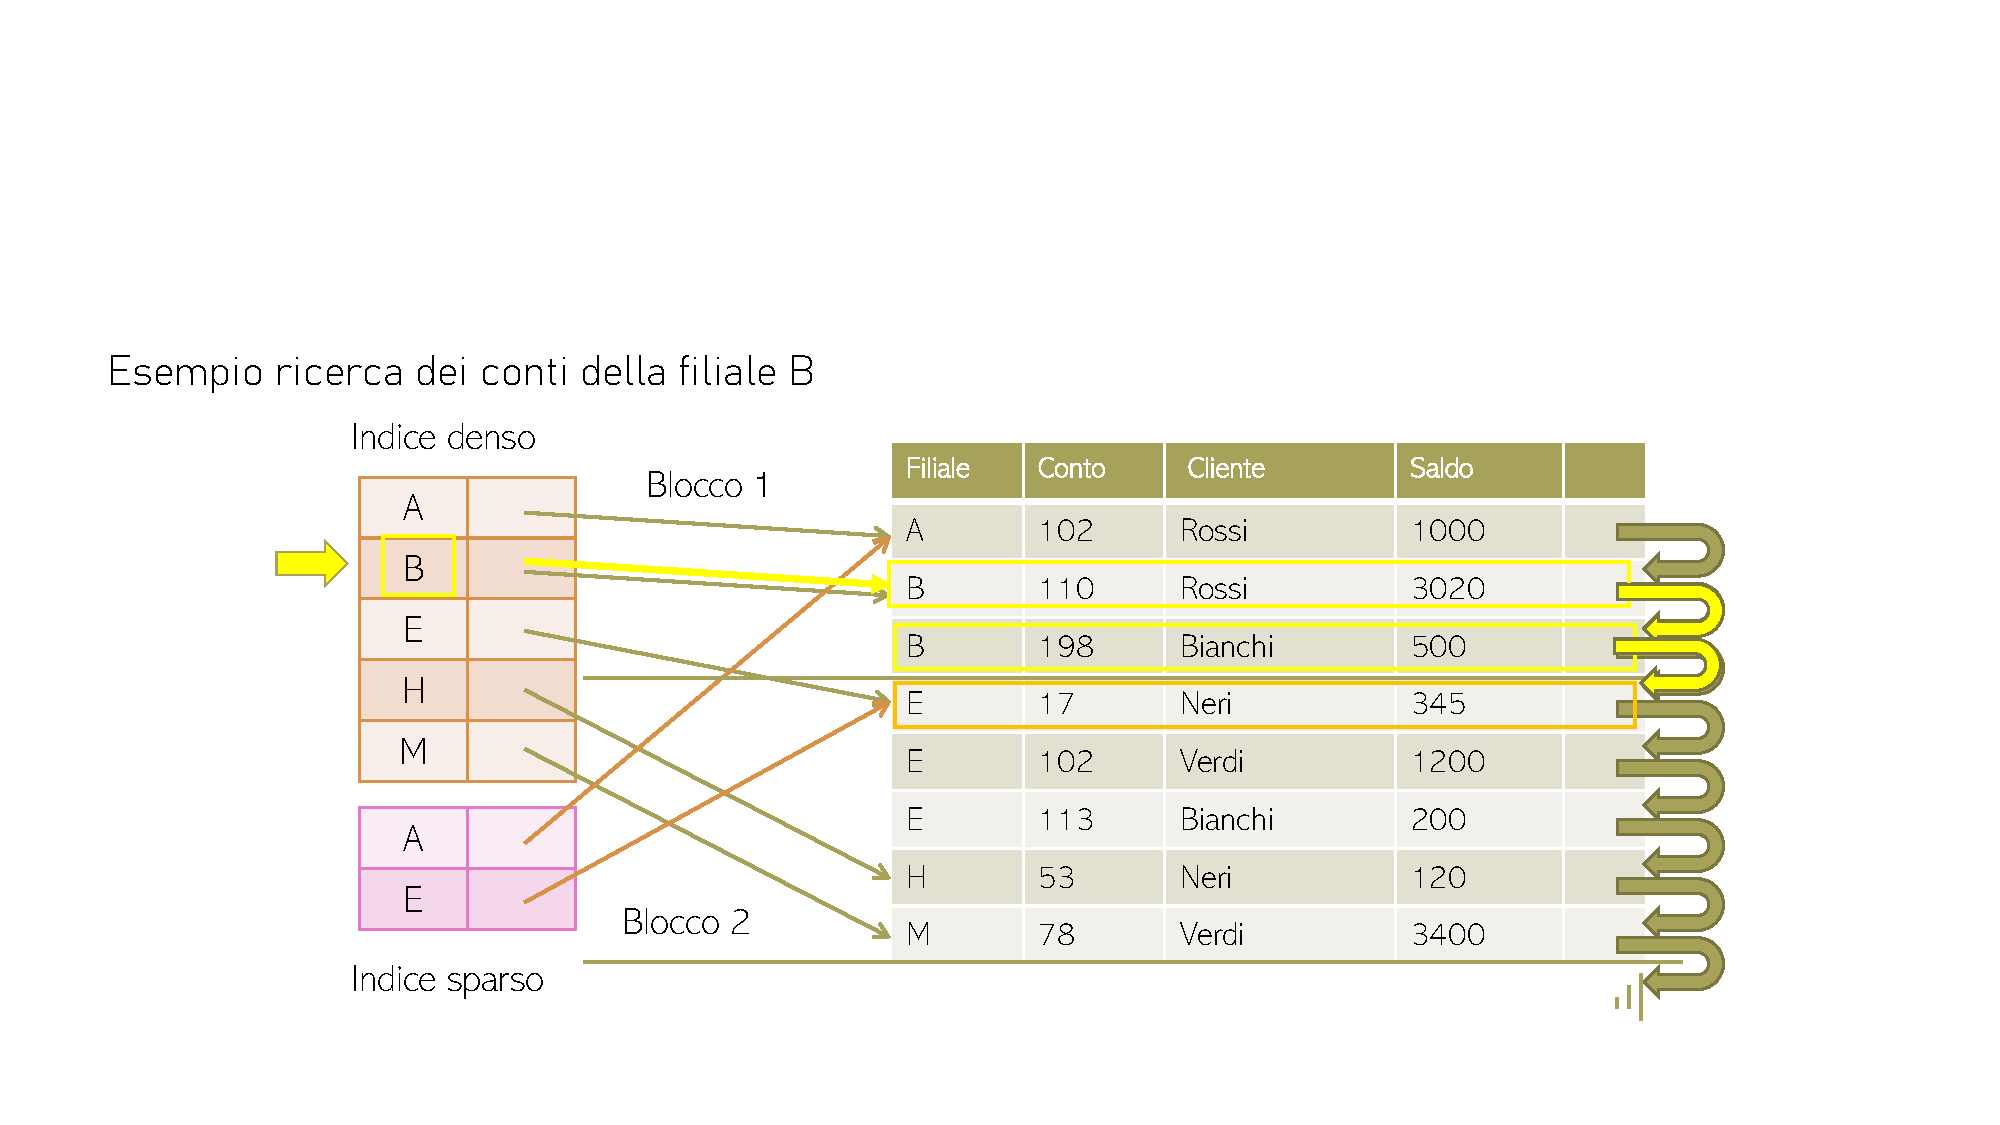
\includegraphics[width=.9\textwidth]{img/ex/indice-denso-2.pdf}
		\end{figure}
		
		\noindent
		Operazione di \textbf{inserimento}: l'inserimento nell'indice avviene solo se la tupla inserita nel file ha un valore di chiave K (chiave di ricerca) che non è già presente.
		
		Operazione di \textbf{cancellazione}: la cancellazione nell'indice avviene solo se la tupla cancellata nel file è l'ultima tupla con valore di chiave K (chiave di ricerca).\newpage
		
		\begin{table}[!htp]
			\centering
			\begin{tabular}{@{} l p{25em} @{}}
				\toprule
				Concetto & Definizione \\
				\midrule
				Definizione 		& Un \textbf{indice primario} utilizza una \textbf{chiave di ricerca che coincide con la chiave di ordinamento} del file sequenziale. Una \textbf{variante} dell'indice primario è l'\underline{indice primario denso}: \textbf{per ogni occorrenza della chiave presente nel file, esiste un corrispondente record nell'indice}. \\ [.7em]
				%
				Op. ricerca 		& Eseguita una \textbf{scansione sequenziale dell'indice} per trovare il record ricercato. \textbf{Se viene trovato}, viene effettuato l'\textbf{accesso al file attraverso il puntatore}. \\ [.7em]
				%
				Op. inserimento		& L'inserimento avviene solo se la \textbf{tupla inserita nel file ha un valore} di chiave K (\textbf{chiave di ricerca}) che \textbf{non} è già \textbf{presente}. \\ [.7em]
				%
				Op. cancellazione	& La cancellazione avviene solo se la \textbf{tupla cancellata nel file è l'ultima tupla con valore di} chiave K (\textbf{chiave di ricerca}). \\
				\bottomrule
			\end{tabular}
			\caption{Riepilogo dei concetti della domanda sull'indice denso.}
		\end{table}
	\end{enumerate}\newpage
	
	Domande di teoria tratte dalla terza prova intermedia dell'esame 07/06/2016.
	\begin{enumerate}
		\item \textbf{(\emph{3 punti})} \textcolor{Green4}{\textbf{\emph{Illustrare l'architettura di un DBMS descrivendo in particolare il modulo di gestione dei guasti (o gestore dell'affidabilità); si indichi inoltre, per ogni modulo dell'architettura, quali sono le proprietà delle transazioni che contribuisce a garantire.}}}\label{dom: gestione dei guasti}
		
		L'architettura di un DBMS è strutturata su 3 livelli differenti:
		\begin{itemize}
			\item Le viste, che appartengono allo schema esterno;
			\item Il modello relazionale, che appartiene allo schema logico;
			\item Le strutture fisiche, che appartengono allo schema interno.
		\end{itemize}
		Lo schema logico comunica con lo schema esterno attraverso l'indipendenza logica e con lo schema interno attraverso l'indipendenza fisica.
		\begin{figure}[!htp]
			\centering
			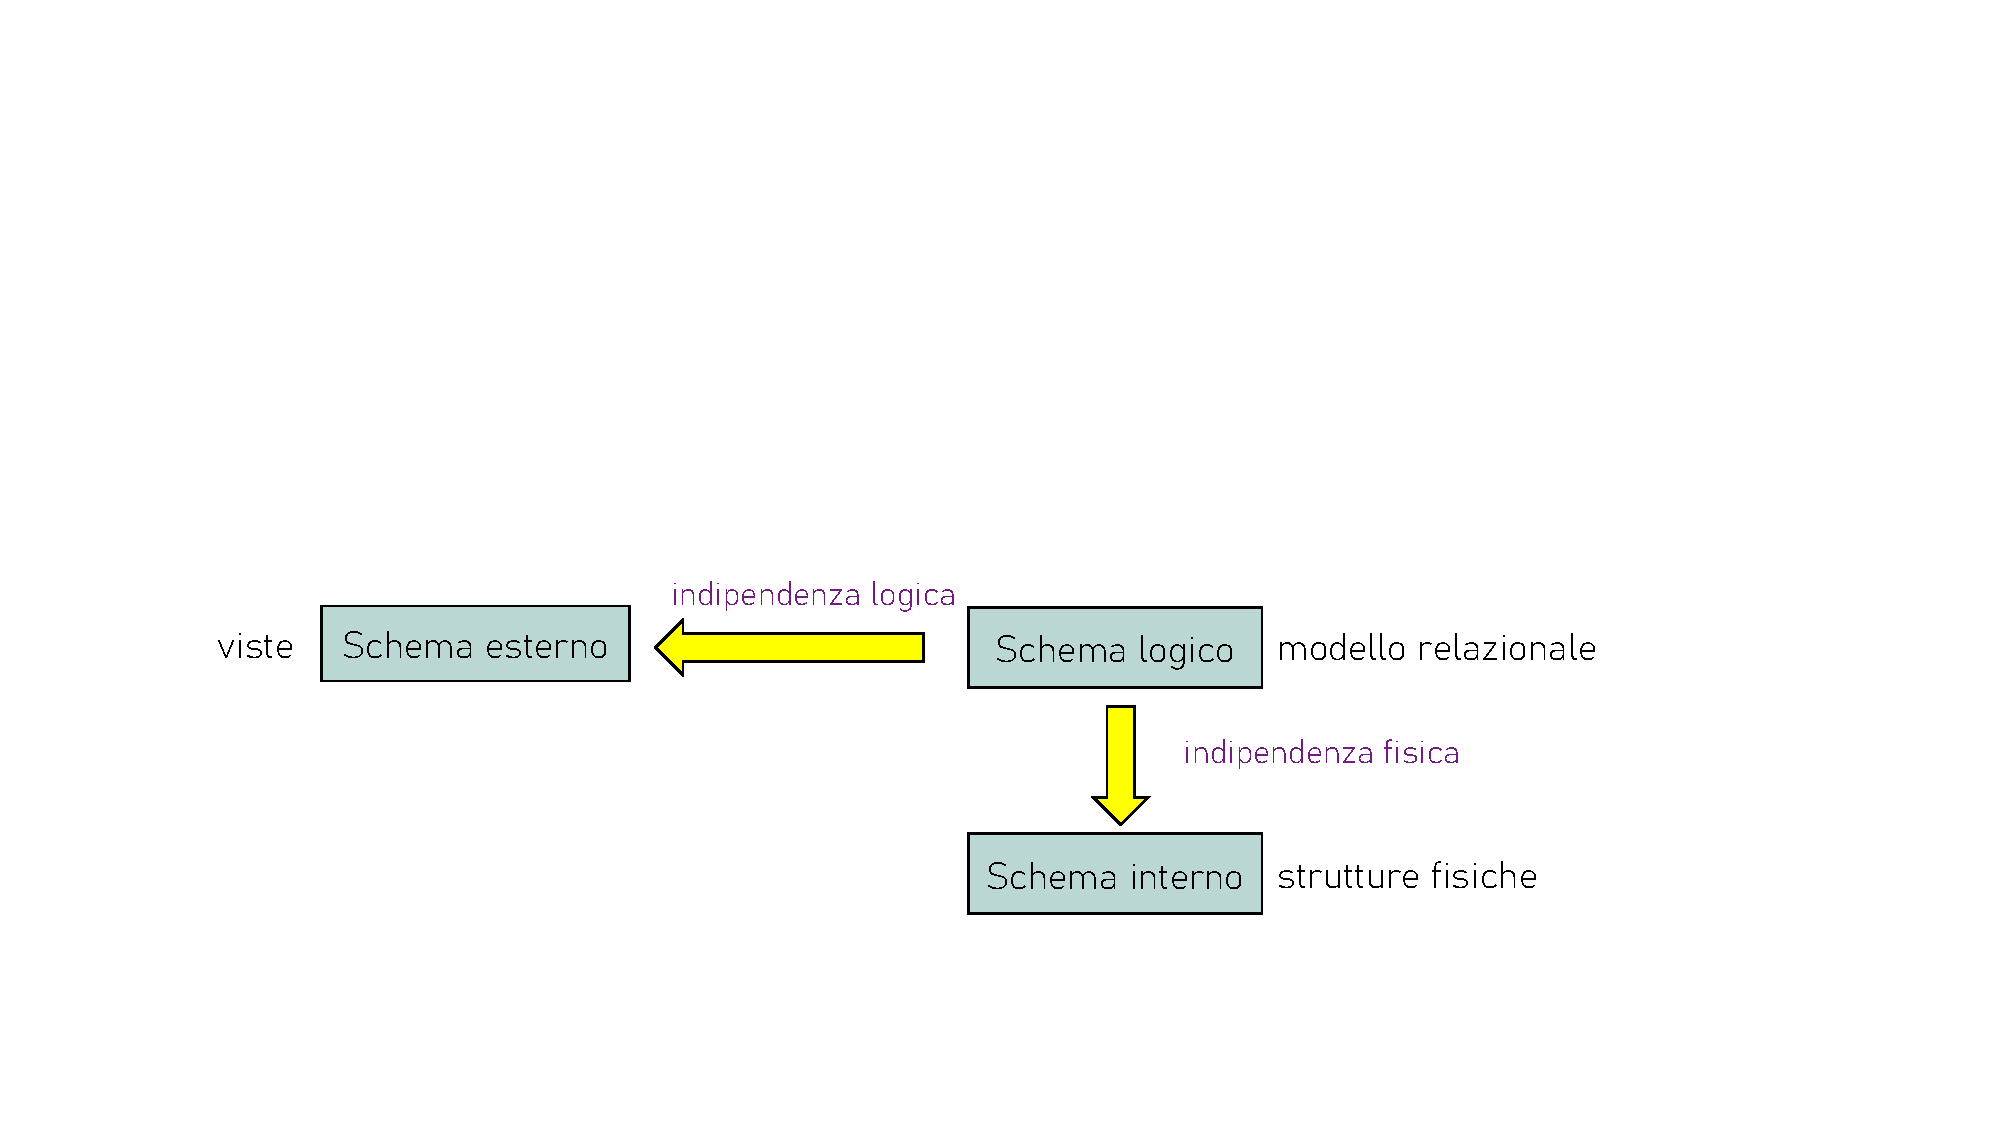
\includegraphics[width=\textwidth]{img/ex/arch-dbms-1.pdf}
		\end{figure}
		
		\noindent
		All'interno dello schema logico ci sono molteplici moduli, i quali garantiscono anche alcune proprietà delle transazioni:
		\begin{itemize}
			\item Gestore delle \textbf{interrogazioni};
			
			\item Gestore dell'\textbf{esecuzione concorrente}, il quale garantisce le proprietà di \underline{atomicità} e \underline{isolamento};
			
			\item Gestore dei \textbf{metodi d'accesso}, il quale garantisce la proprietà di \underline{consistenza};
			
			\item Gestore dell'\textbf{affidabilità}, il quale garantisce \underline{atomicità} e \underline{persistenza};
			
			\item Gestore del \textbf{buffer};
			
			\item Gestore della \textbf{memoria secondaria}.
		\end{itemize}
		Ricapitolando:
		\begin{table}[!htp]
			\centering
			\begin{tabular}{@{} l p{18em} @{}}
				\toprule
				Proprietà & Garantita da \\
				\midrule
				\textbf{Atomicità} 	& Gestore dell'\textbf{esecuzione concorrente} \newline Gestore dell'\textbf{affidabilità} \\ [0.5em]
				\textbf{Consistenza}	& Gestore dei \textbf{metodi d'accesso} \\ [0.5em]
				\textbf{Isolamento} 	& Gestore dell'\textbf{esecuzione concorrente} \\ [0.5em]
				\textbf{Persistenza} & Gestore dell'\textbf{affidabilità} \\
				\bottomrule
			\end{tabular}
		\end{table}\newpage
		\begin{figure}[!htp]
			\centering
			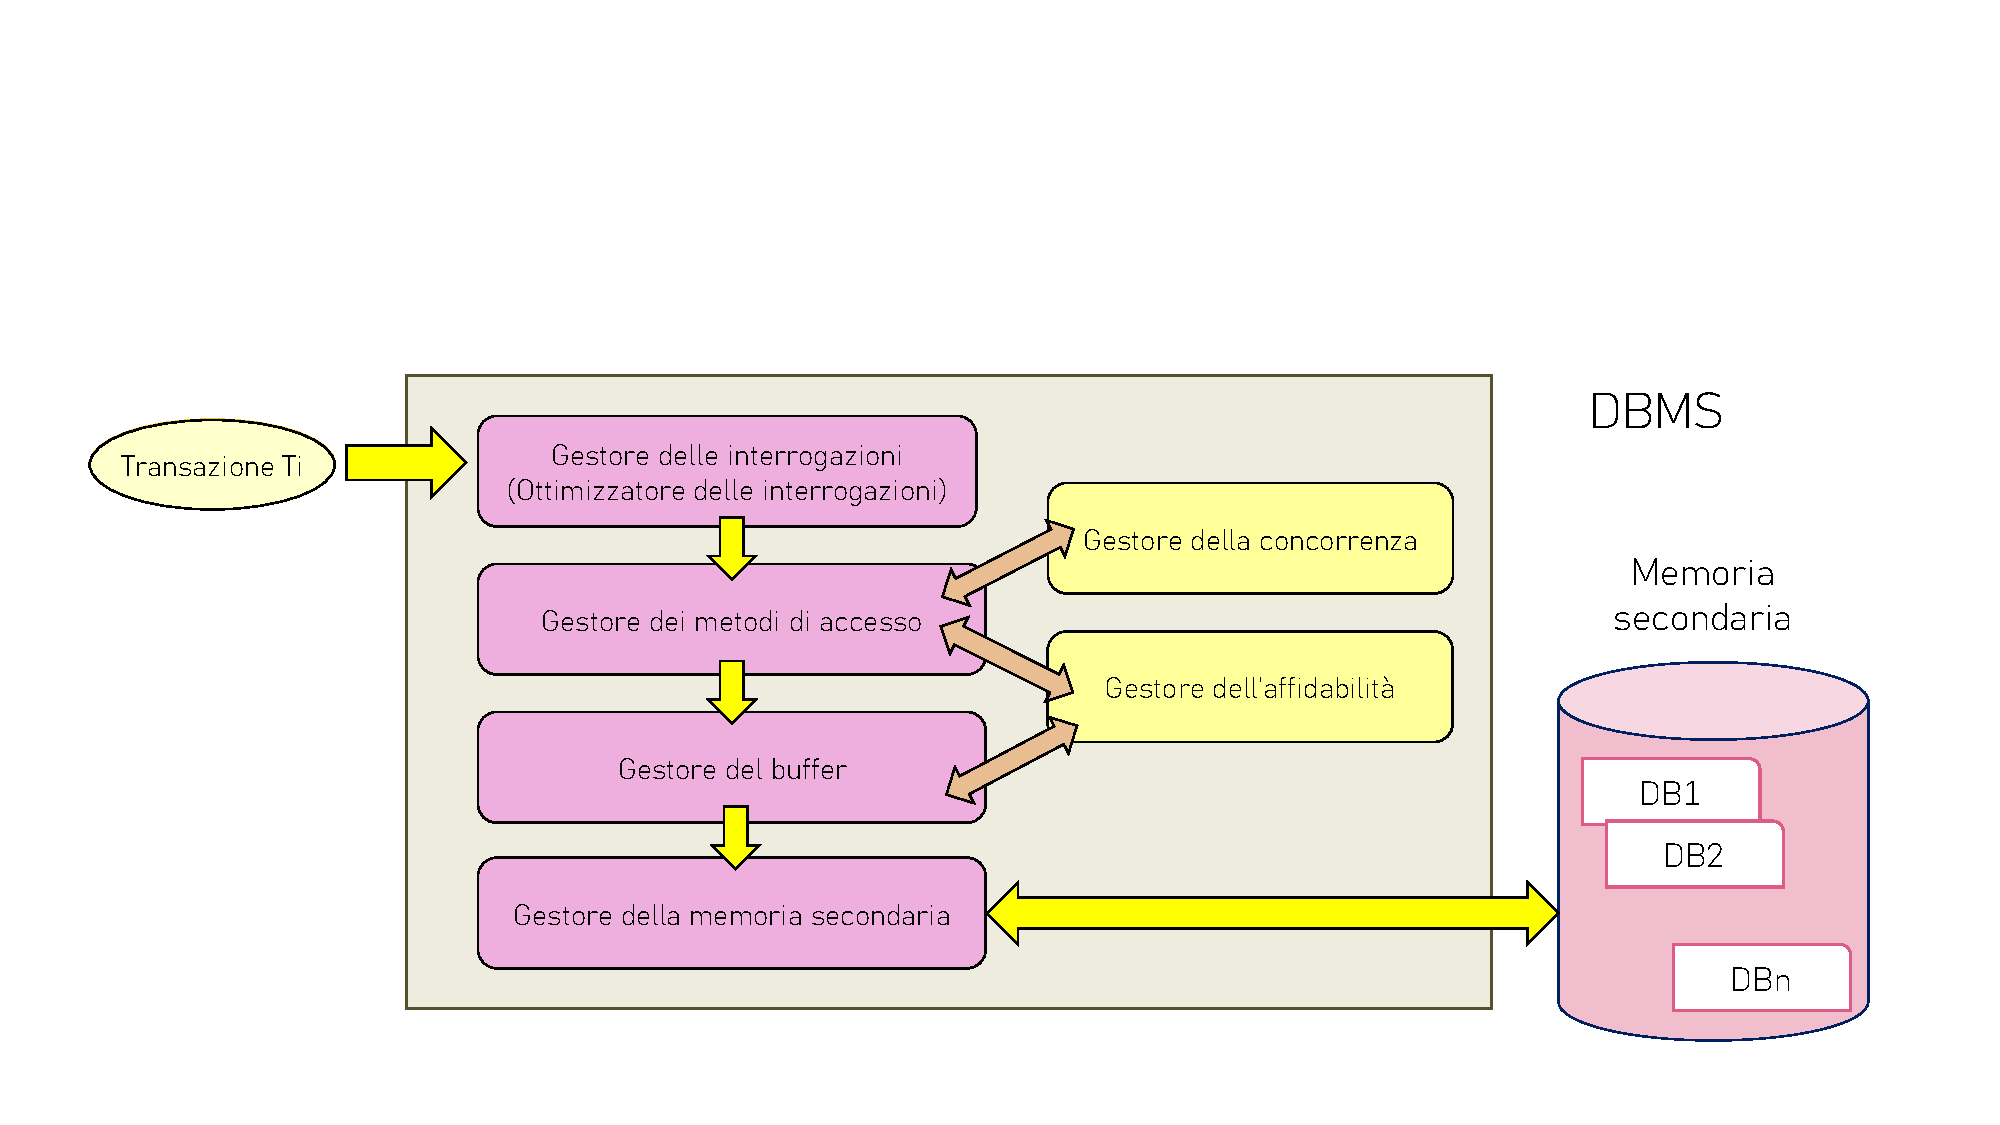
\includegraphics[width=\textwidth]{img/ex/arch-dbms-2.pdf}
		\end{figure}
		
		\noindent
		Il \textbf{modulo di gestione dei guasti}, o \textbf{gestore dell'affidabilità}, garantisce due \textbf{proprietà fondamentali}:
		\begin{itemize}
			\item \textbf{Atomicità}, garantire che le \textbf{transazioni non vengano lasciate incomplete};
			
			\item \textbf{Persistenza}, garantire che gli \textbf{effetti di ciascuna transazione conclusa con un \emph{commit} siano mantenuti in modo permanente}.
		\end{itemize}
		Le \textbf{proprietà} vengono \textbf{garantite grazie ai log}, ovvero un \textbf{archivio persistente su cui vengono registrate le varie azioni svolte dal DBMS}.
		
		Il gestore dell'affidabilità utilizza delle primitive (\textsf{force, fix, unfix, setDirty}) per comunicare con il gestore del buffer. Questo perché esso invia \textbf{richieste di accessi a pagine in lettura/scrittura al \emph{buffer manager}}, e genera \textbf{ulteriori richieste di lettura/scrittura necessarie a garantire la robustezza e resistenza ai guasti}.
		
		Infine, date le proprietà che deve garantire, questo \textbf{componente necessita di una memoria stabile}, \textbf{ovvero di una memoria resistente ai guasti}.
		
		\begin{figure}[!htp]
			\centering
			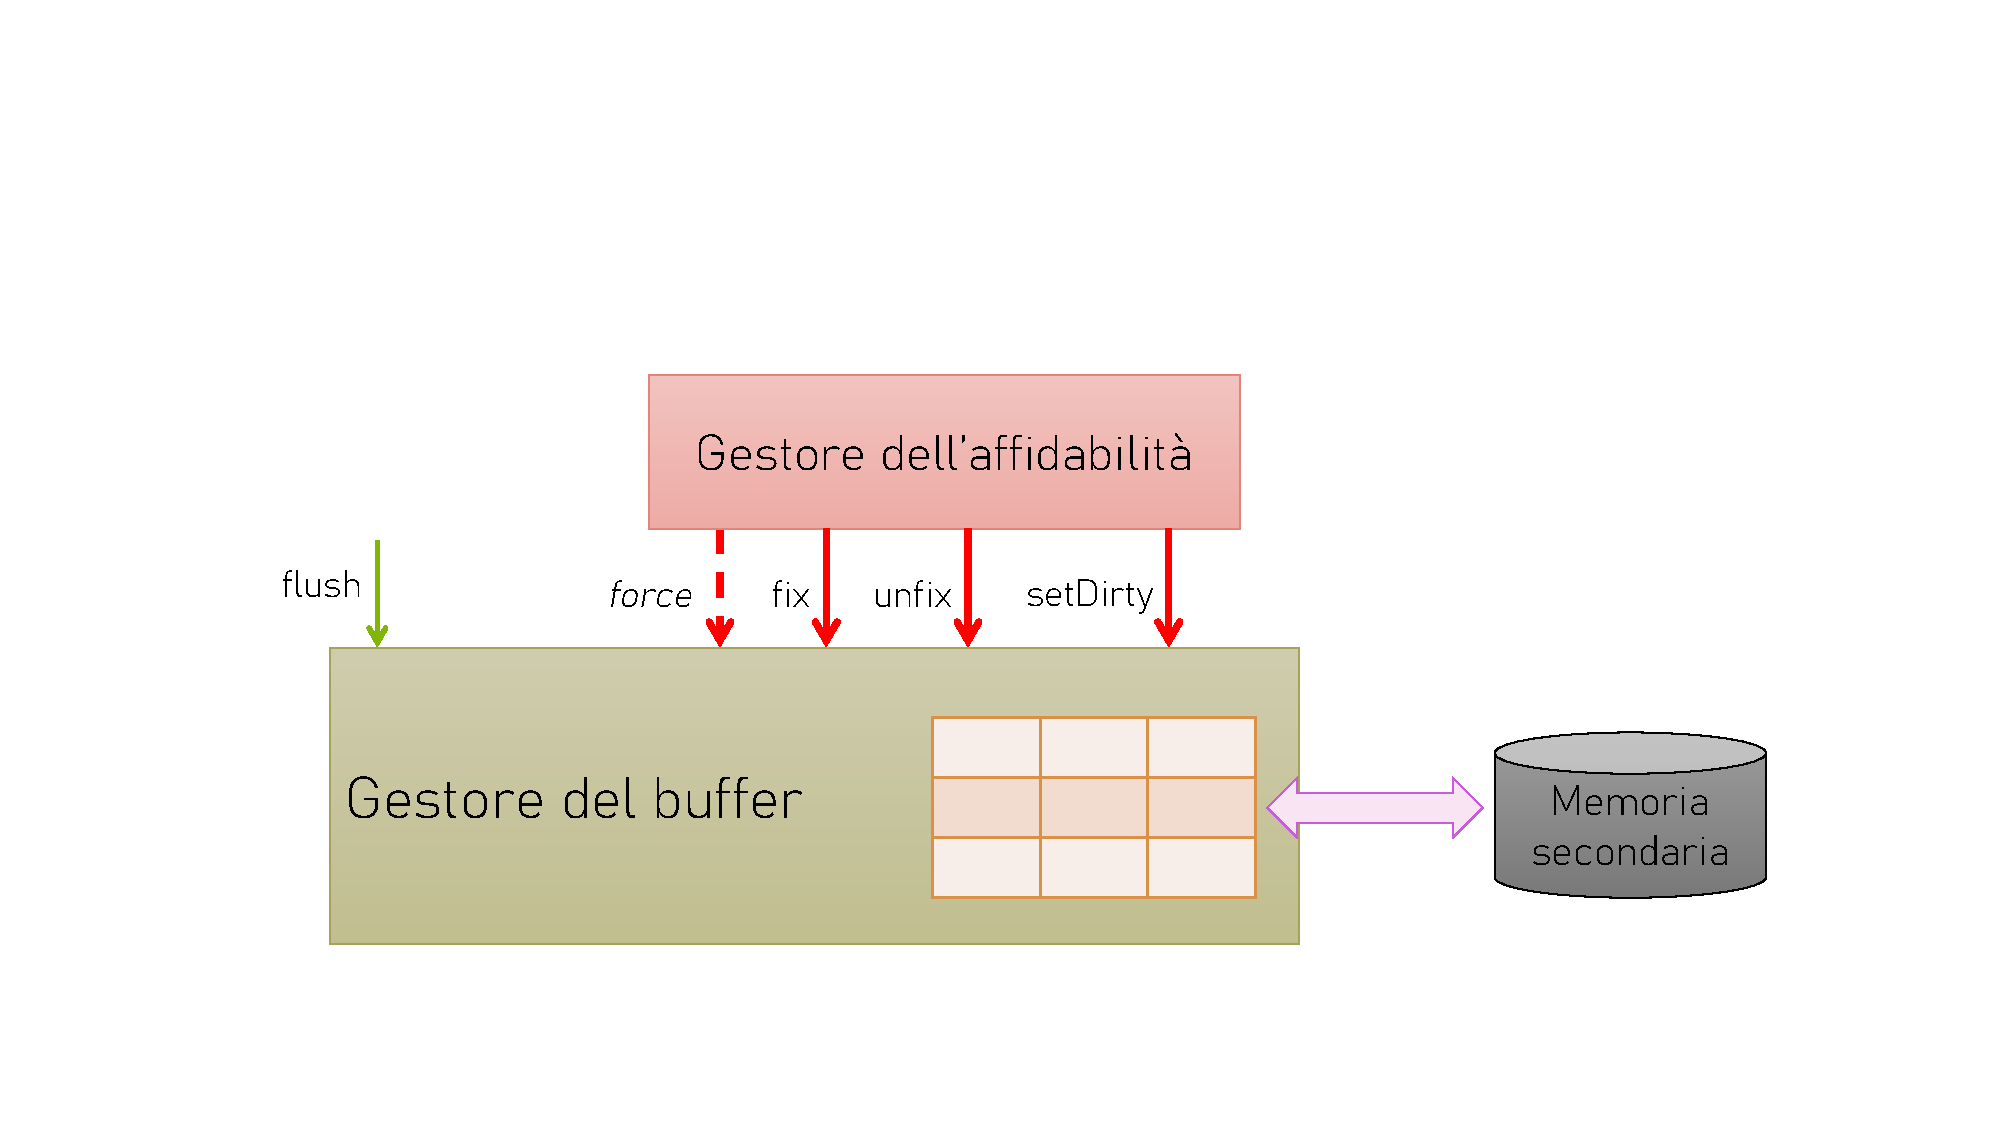
\includegraphics[width=\textwidth]{img/ex/gestore-dei-guasti-1.pdf}
		\end{figure}\newpage
		
		\begin{table}[!htp]
			\centering
			\begin{tabular}{@{} l p{23em} @{}}
				\toprule
				Concetto & Definizione \\
				\midrule
				Architettura DBMS & L'architettura DBMS è strutturata su \textbf{3 livelli}: schema \textbf{esterno}, \textbf{logico} e \textbf{interno}. Lo schema \textbf{logico}, \textbf{il più importante}, ha al suo interno una serie di \textbf{moduli} (gestori) importanti: delle \textbf{interrogazioni}, dell'\textbf{esecuzione concorrente}, dei \textbf{metodi d'accesso}, dell'\textbf{affidabilità}, del \textbf{buffer}, della \textbf{memoria secondaria}. \\ [.7em]
				%
				Proprietà garantite & A sinistra le proprietà e a destra i moduli che le garantiscono:
				\begin{equation*}
					\begin{array}{lll}
						\textbf{Atomicità}	&\rightarrow& \text{Gestore esecuzione concorrente,} \\
						&			& \text{Gestore dell'affidabilità} \\ [.5em]
						\textbf{Consistenza}&\rightarrow& \text{Gestore dei metodi d'accesso} \\ [.5em]
						\textbf{Isolamento}	&\rightarrow& \text{Gestore esecuzione concorrente} \\ [.5em]
						\textbf{Persistenza}&\rightarrow& \text{Gestore dell'affidabilità}
					\end{array}
				\end{equation*} \\ [.7em]
				%
				Approfondimento proprietà & L'\textbf{\underline{atomicità}} garantisce che le transazioni non vengano lasciate incomplete. Invece, la \textbf{\underline{persistenza}} garantisce che gli effetti di ciascuna transazione conclusa con un commit siano mantenuti in modo permanente. Queste \textbf{proprietà} sono \textbf{garantite dal modulo di gestione dei guasti} grazie al \underline{log}, ovvero un \textbf{archivio persistente} su cui vengono \textbf{registrate} le varie \textbf{azioni svolte dal DBMS}. \\ [.7em]
				%
				Compito eseguito & Il modulo di gestione dei guasti invia \textbf{richieste di accessi a pagine in lettura/scrittura al buffer}.\newline
				Inoltre, genera \textbf{ulteriori richieste di lettura/scrittura necessarie a garantire la robustezza e resistenza ai guasti}. \\
				\bottomrule
			\end{tabular}
			\caption{Riepilogo dei concetti della domanda sull'indice denso.}
		\end{table}\newpage
		
		\item \textbf{(\emph{3 punti})} \textcolor{Green4}{\textbf{\emph{Si presenti in dettaglio la \underline{politica di concessione dei lock} applicata dal gestore dell'esecuzione concorrente secondo la tecnica detta \dquotes{Locking a due fasi}.}}}\label{dom: politica di concessione dei lock - locking a due fasi}
		
		Il \emph{\textbf{locking}} è una tecnica in cui \textbf{tutte le operazioni di lettura/scrittura devono essere protette tramite l'esecuzione di opportune primitive} (\textsf{r\_lock}, \textsf{w\_lock}, \textsf{unlock}). Quindi, lo \textbf{scheduler riceve una sequenza di richieste di esecuzione di queste primitive da parte delle transazioni, e ne determina la correttezza con una semplice ispezione di una struttura dati}.
		
		Il \textbf{gestore della concorrenza mantiene per ogni risorsa}: il suo \underline{\textbf{stato}} (identificato tramite le tre primitive), le transazioni in \textsf{r\_lock}, ovvero tutte le transazioni che hanno un \textsf{r\_lock} sulla risorsa x. Inoltre, viene salvata una \textbf{tabella dei conflitti} in cui:
		\begin{itemize}
			\item Le \textbf{righe} identificano le \textbf{richieste};
			
			\item Le \textbf{colonne} identificano lo \textbf{stato della risorsa richiesta};
			
			\item In ogni \textbf{cella}:
			\begin{itemize}
				\item Valore di \textbf{sinistra} identifica l'\textbf{esito della richiesta};
				
				\item Valore di \textbf{destra} identifica lo \textbf{stato} che verrà assunto dalla \textbf{risorsa dopo l'esecuzione della primitiva}.
			\end{itemize}
		\end{itemize}
		
		Grazie a questa tabella, il lock manager ha la possibilità di scegliere quando concedere o non concedere una risorsa in lettura/scrittura:
		\begin{itemize}
			\item \textbf{Oggetto} bloccato in \textbf{lettura}, allora è possibile \textbf{concedere un'altra richiesta di lock in lettura} (\emph{lock condiviso});
			
			\item Nel caso di \textsf{unlock} di una \textbf{risorsa bloccata} in modo condiviso (lettura), la \textbf{risorsa ritorna libera quando non ci sono altre transazioni in lettura che operano su di essa}.
		\end{itemize}\newpage
		
		\begin{table}[!htp]
			\centering
			\begin{tabular}{@{} l p{21em} @{}}
				\toprule
				Concetto & Definizione \\
				\midrule
				Definizione locking & Il \emph{\textbf{locking}} è una tecnica in cui \textbf{tutte le operazioni di lettura/scrittura devono essere protette tramite l'esecuzione di opportune primitive} (\textsf{r\_lock}, \textsf{w\_lock}, \textsf{unlock}). \\ [.7em]
				%
				Politica di concessione & Il \textbf{gestore della concorrenza mantiene per ogni risorsa}: il suo \underline{\textbf{stato}} (identificato tramite le tre primitive), le transazioni in \textsf{r\_lock}, ovvero \textbf{tutte le transazioni che hanno un \textsf{r\_lock} sulla risorsa x}. \\ [.7em]
				%
				Tabella dei conflitti & Salvata una \textbf{tabella dei conflitti} in cui:
				\begin{itemize}
					\item Le \textbf{righe} identificano le \textbf{richieste};
					
					\item Le \textbf{colonne} identificano lo \textbf{stato della risorsa richiesta};
					
					\item In ogni \textbf{cella}:
					\begin{itemize}
						\item Valore di \textbf{sinistra} identifica l'\textbf{esito della richiesta};
						
						\item Valore di \textbf{destra} identifica lo \textbf{stato} che verrà assunto dalla \textbf{risorsa dopo l'esecuzione della primitiva}.
					\end{itemize}
				\end{itemize} \\ [.7em]
				%
				Concessione risorse & È possibile \textbf{scegliere quando concedere o non concedere una risorsa} in lettura/scrittura:
				\begin{itemize}
					\item \textbf{Oggetto} bloccato in \textbf{lettura}, allora è possibile \textbf{concedere un'altra richiesta di lock in lettura} (\emph{lock condiviso});
					
					\item Nel caso di \textsf{unlock} di una \textbf{risorsa bloccata} in modo condiviso (lettura), la \textbf{risorsa ritorna libera quando non ci sono altre transazioni in lettura che operano su di essa}.
				\end{itemize} \\
				\bottomrule
			\end{tabular}
			\caption{Riepilogo dei concetti della domanda sulla politica di concessione dei lock.}
		\end{table}\newpage
		
		\item \textbf{(\emph{2 punti})} \textcolor{Green4}{\textbf{\emph{Lo studente illustri la struttura di accesso ai dati denominata indice primario sparso, si descrivano in particolare i seguenti punti: (i) le caratteristiche della struttura di accesso, (ii) l'algoritmo di ricerca di una tupla con chiave K usando l'indice.}}}\label{dom: indice primario sparso}
		
		Un indice primario utilizza una chiave di ricerca che coincide con la chiave di ordinamento del file sequenziale. Esistono due varianti dell'indice primario, una di queste è l'\textbf{indice sparso}: \textbf{solo per alcune occorrenze della chiave presenti nel file esiste un corrispondente record nell'indice, tipicamente una per blocco}.
		\begin{figure}[!htp]
			\centering
			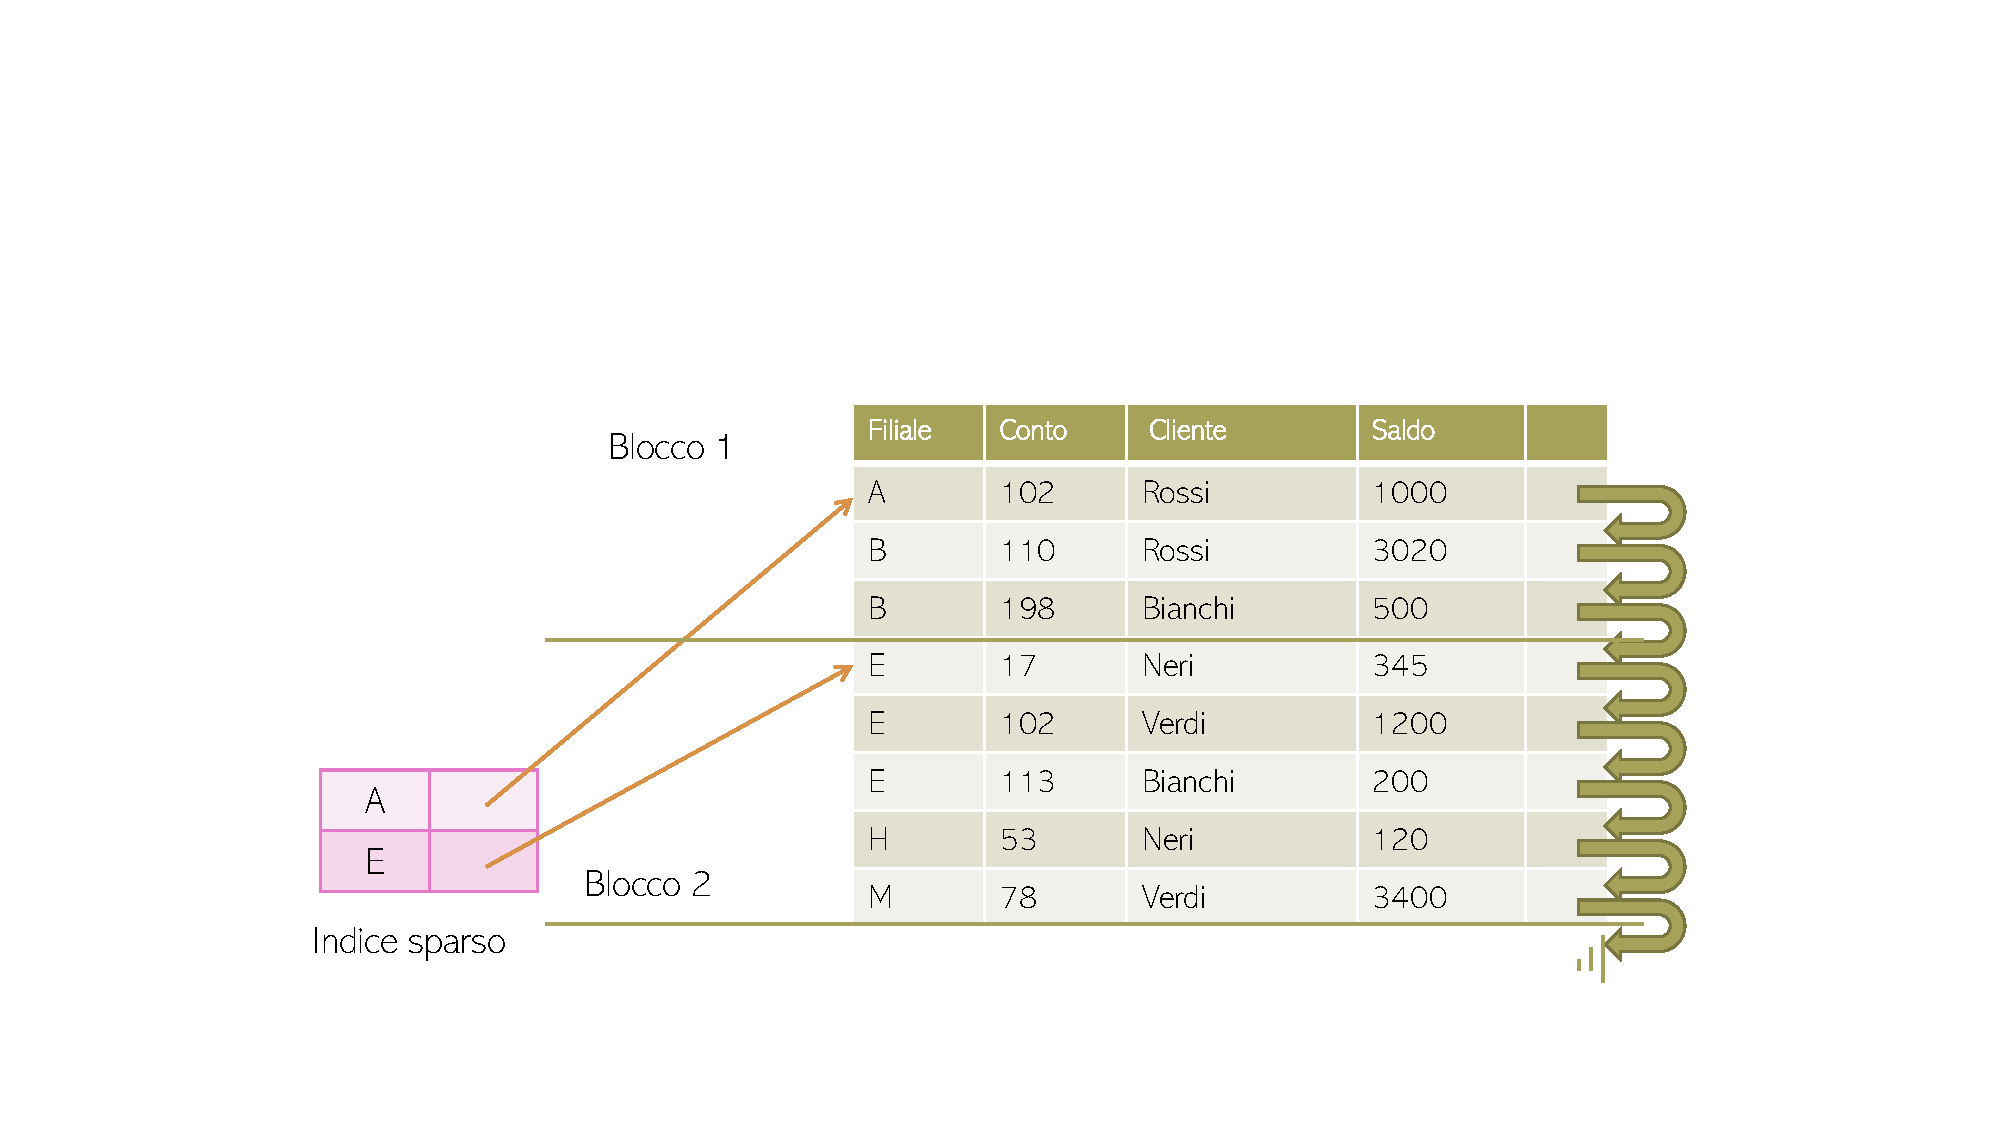
\includegraphics[width=\textwidth]{img/ex/indice-sparso-1.pdf}
		\end{figure}
		
		\noindent
		\textbf{Operazione di ricerca} con una chiave K:
		\begin{enumerate}
			\item Eseguita una \textbf{scansione sequenziale dell'indice}. La scansione termina quando viene trovato un \textbf{record che ha come chiave il valore più grande}, ma che è comunque \textbf{minore o uguale alla chiave di ricerca} K;
			
			\item Eseguito l'\textbf{accesso al file attraverso il puntatore all'interno del record}, ed eseguita la \textbf{scansione del file} (blocco corrente) \textbf{per trovare le tuple con chiave} K.
		\end{enumerate}
		\textbf{N.B.:} si cerca il valore di chiave più grande $\ge$ K, poiché data la struttura dell'indice sparso, la chiave K potrebbe non essere presente nell'indice.
		\begin{equation*}
			\text{Costo totale} = 1 \text{ accesso indice } + 1 \text{ accesso blocco dati }
		\end{equation*}\newpage
		s
		\begin{figure}[!htp]
			\centering
			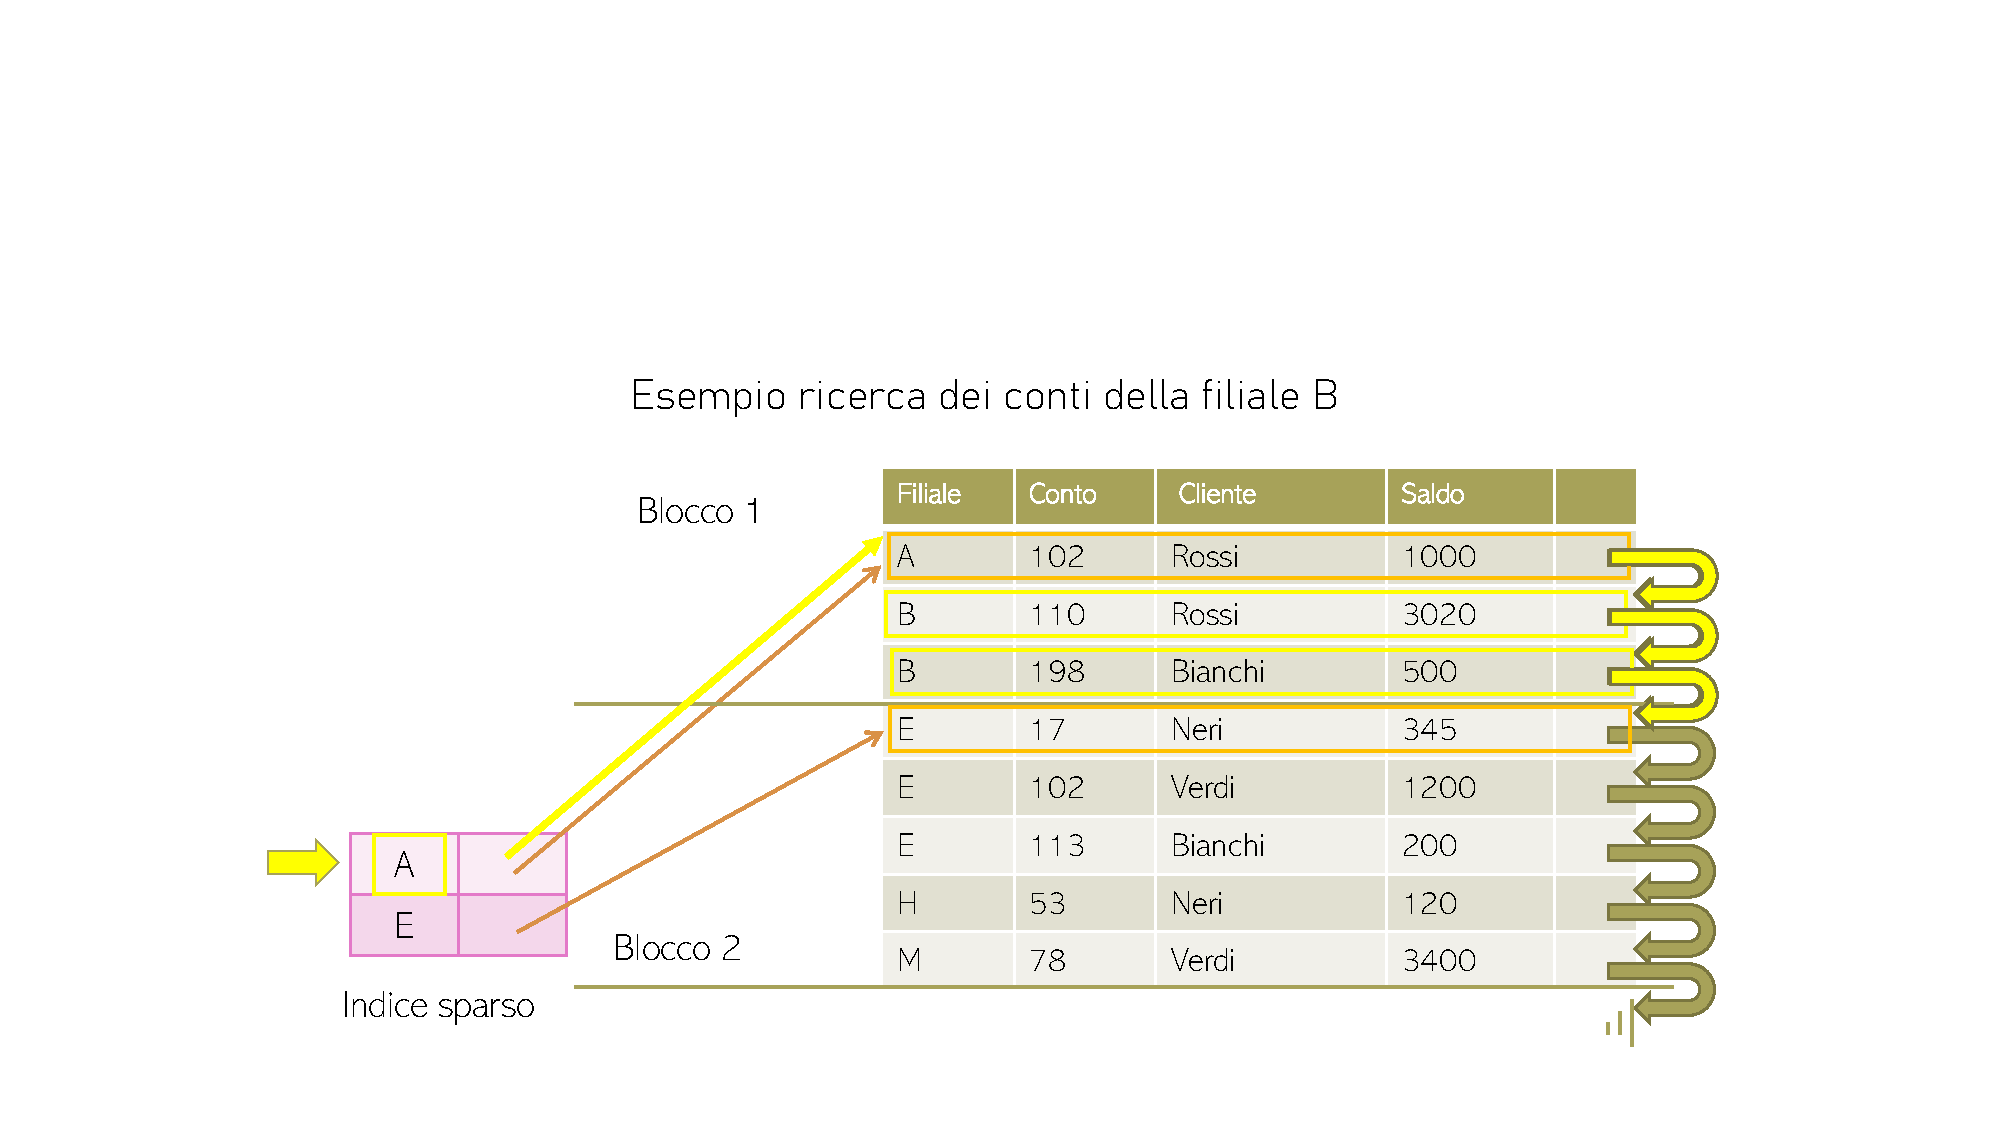
\includegraphics[width=\textwidth]{img/ex/indice-sparso-2.pdf}
		\end{figure}
		
		\begin{table}[!htp]
			\centering
			\begin{tabular}{@{} l p{24em} @{}}
				\toprule
				Concetto & Definizione \\
				\midrule
				Definizione & Un \textbf{indice primario} utilizza una \textbf{chiave di ricerca che coincide con la chiave di ordinamento} del file sequenziale. Una \textbf{variante} dell'indice primario è l'\underline{indice primario sparso}: \textbf{solo per alcune occorrenze delle chiavi presenti nel file esiste un corrispondente record nell'indice, tipicamente una per blocco}. \\ [.7em]
				%
				Op. ricerca & La ricerca si divide in due fasi:
				\begin{enumerate}
					\item Esecuzione di una \textbf{scansione sequenziale dell'indice}. La scansione termina quando viene trovato un \textbf{record che ha come chiave il valore più grande}, ma che è comunque \textbf{minore o uguale alla chiave di ricerca} K;
					
					\item \textbf{Accesso al file attraverso il puntatore all'interno del record}, e \textbf{scansione del file} (blocco corrente) \textbf{per trovare le tuple con chiave} K.
				\end{enumerate} \\
				\bottomrule
			\end{tabular}
			\caption{Riepilogo dei concetti della domanda sull'indice sparso.}
		\end{table}\newpage
		
		\item \textbf{(\emph{2 punti})} \textcolor{Green4}{\textbf{\emph{Lo studente illustri le differenze tra i costrutti \textbf{elemento} e \textbf{attributo} del linguaggio XML, mostrando un esempio di documento XML dove vengono utilizzati entrambi.}}}\label{dom: elemento e attributo in XML}
		
		Un \textbf{elemento} è tutto ciò che viene compreso tra il tag di inizio e il tag di fine e la keyword \textsf{element} li identifica in uno schema XML. Esistono varie modalità per dichiarare un elemento e inoltre possono essere eseguite dichiarazioni annidate.
		
		Un \textbf{attributo} è un valore \underline{opzionale} che aggiunge informazioni ad un elemento. Solitamente viene utilizzato per rappresentare dei valori unici come gli ID.
		
		Date le due definizioni, le \textbf{maggiori differenze} sono:
		\begin{itemize}
			\item La \textbf{dichiarazione di attributi deve avvenire sempre dopo la dichiarazione di elementi} (\underline{non viceversa}).
			
			\item Un \textbf{attributo} può contenere \textbf{solo un valore}, mentre gli \textbf{elementi possono avere figli}.
		\end{itemize}
		Un esempio di codice XML:
		\begin{lstlisting}[language=XML]
<xsd:element name="Book">
	<xsd:complexType>
		<xsd:element name="Title" type="xsd:string"/>
		<xsd:element name="Author" type="xsd:string">
			<xsd:complexType>
				<xsd:attribute 	name="author_id" type="xsd:ID" use="required"/>
			</xsd:complexType>
		</xsd:element>
		<xsd:element name="Date" type="xsd:gYear"/>
	</xsd:complexType>
</xsd:element>\end{lstlisting}
	\end{enumerate}
	
	\noindent
	\begin{table}[!htp]
		\centering
		\begin{tabular}{@{} l p{22em} @{}}
			\toprule
			Concetto & Definizione \\
			\midrule
			Breve def. elemento		& Un \textbf{elemento} è tutto ciò che viene compreso tra il tag di inizio e il tag di fine. Viene identificato dalla keyword \textsf{element} nel XML schema. \\ [.5em]
			%
			Breve def. attributo	& Un \textbf{attributo} è un valore \underline{opzionale} che aggiunge informazioni ad un elemento. Utilizzato per rappresentare gli ID di solito. \\ [.5em]
			%
			Differenze				& Due differenze sostanziali: (1) la \textbf{dichiarazione di attributi deve avvenire sempre dopo la dichiarazione di elementi} (\underline{non viceversa}); (2) un \textbf{attributo} può contenere \textbf{solo un valore}, mentre gli \textbf{elementi possono avere figli}.\\ [.5em]
			%
			Esempio					& Si veda il codice sopra. \\
			\bottomrule
		\end{tabular}
		\caption{Riepilogo dei concetti della domanda sull'elemento e l'attributo in XML.}
	\end{table}\newpage
	
	Domande di teoria tratte dalla terza prova intermedia dell'esame 21/04/2022.
	\begin{enumerate}
		\item \textbf{(\emph{3 punti})} \textcolor{Green4}{\textbf{\emph{Illustrare l'architettura di un DBMS descrivendo in particolare il modulo di gestione dei buffer; si indichi inoltre quali moduli garantiscono le proprietà di persistenza e consistenza delle transazioni.}}}
		
		Risposta a pagina \pageref{dom: gestione del buffer}.
		
		\item \textbf{(\emph{2 punti})} \textcolor{Green4}{\textbf{\emph{Si presenti in dettaglio la \underline{definizione di conflict-equivalenza} tra due schedule.}}}\label{dom: conflict-equivalenza}
		
		Prima della definizione di conflict-equivalenza, è necessario dire cosa è un conflitto.
		
		Date due azioni eseguite da transazioni diverse, si dice che un'azione è in \textbf{conflitto} con un'altra, se \textbf{operano sullo stesso oggetto} e almeno \textbf{una di esse è in scrittura}. I conflitti che si possono creare quindi sono: lettura-scrittura, scrittura-lettura, scrittura-scrittura.
		
		Uno schedule è definito \textbf{conflict-equivalente} ad un altro schedule, se \textbf{entrambi presentano le stesse operazioni} e ogni \textbf{coppia di operazioni in conflitto è nello stesso ordine} in entrambi gli schedule.
		
		\begin{table}[!htp]
			\centering
			\begin{tabular}{@{} l p{20em} @{}}
				\toprule
				Concetto & Descrizione \\
				\midrule
				Def. conflitto				& \textbf{Due azioni} di \textbf{due transazioni} \underline{diverse} sono in \textbf{conflitto} se operano sullo \textbf{stesso oggetto} e almeno una di esse è \textbf{una scrittura}. \\ [.7em]
				Def. conflict-equivalenza 	& \textbf{Due schedule} sono \textbf{conflict-equivalenti} se:
				\begin{itemize}
					\item Hanno le \textbf{stesse operazioni}
					
					\item Ogni coppia di \textbf{operazioni in conflitto} è nello \textbf{stesso ordine} nei due schedule
				\end{itemize}\\
				\bottomrule
			\end{tabular}
			\caption{Riepilogo dei concetti della domanda sulla conflict-equivalenza.}
		\end{table}\newpage
		
		\item \textbf{(\emph{2 punti})} \textcolor{Green4}{\textbf{\emph{Lo studente illustri la struttura di accesso ai dati denominata struttura ad accesso calcolato (hashing), si descrivano in particolare i seguenti punti: (i) le caratteristiche della struttura di accesso, (ii) l'algoritmo di ricerca di una tupla con chiave K usando l'indice.}}}\label{dom: struttura ad accesso calcolato - hashing}
		
		Le \textbf{strutture ad accesso calcolato} (hashing), si basano su una \textbf{funzione di hash che esegue un \emph{mapping}} dei \textbf{valori chiave di ricerca} sugli \textbf{indirizzi di memorizzazione delle tuple} nelle pagine della memoria secondaria.
		
		Un \textbf{utilizzo efficiente} della funzione di hash prevede la \textbf{distribuzione dei valori delle chiavi} in maniera \underline{uniforme}, \underline{casuale} e all'\underline{interno dei \emph{bucket}}.
		
		Operazione di \textbf{ricerca}:
		\begin{enumerate}
			\item (nessun costo) \textbf{Calcolo la funzione di hash}
			
			\item (1 per ogni pagina) \textbf{Accedo al bucket} ottenuto dalla funzione hash del punto precedente
			
			\item (costo uguale agli accessi per pagina) \textbf{Accedo alle tuple attraverso i puntatori del bucket}
		\end{enumerate}
		
		\begin{table}[!htp]
			\centering
			\begin{tabular}{@{} l p{27em} @{}}
				\toprule
				Concetto & Descrizione \\
				\midrule
				Definizione & Le \textbf{strutture di accesso calcolato} si basano su una \textbf{funzione di hash} che ha l'obbiettivo di \textbf{eseguire un mapping} tra:
				\begin{equation*}
					\text{Chiavi di ricerca} \longrightarrow \text{Indirizzi di memorizzazione delle tuple}
				\end{equation*} \\ 
				%
				Struttura	& La \textbf{distribuzione delle chiavi} deve essere eseguita in modo:
				\begin{itemize}
					\item \textbf{Uniforme}
					\item \textbf{Casuale}
					\item All'\textbf{interno dei \emph{bucket}}
				\end{itemize}
				In questo modo vi è un utilizzo efficiente. \\ [1em]
				%
				Op. ricerca	& L'operazione di ricerca si divide in 3 punti:
				\begin{enumerate}
					\item \textbf{Calcolo della funzione hash}
					
					\item \textbf{Accesso al \emph{bucket}} con il risultato del punto 1
					
					\item \textbf{Accesso alle tuple} attraverso i puntatori del \emph{bucket}
				\end{enumerate} \\
				\bottomrule
			\end{tabular}
			\caption{Riepilogo dei concetti della domanda sulla struttura ad accesso calcolato (hashing).}
		\end{table}\newpage
		
		\item \textbf{(\emph{2 punti})} \textcolor{Green4}{\textbf{\emph{Lo studente illustri l'algoritmo di \underline{ripresa a caldo}.}}}\label{dom: ripresa a caldo}
		
		L'\textbf{algoritmo} è il seguente:
		\begin{enumerate}
			\item Eseguito l'accesso all'ultimo log, ovvero quello al momento del guasto;
			
			\item Si ripercorre l'intero log all'indietro finché non viene trovato l'ultimo checkpoint;
			
			\item Creazione di due insiemi:
			\begin{itemize}
				\item UNDO (rifare) inizializzato con le transazioni attive al checkpoint
				
				\item REDO (disfare) inizializzato con l'insieme vuoto
			\end{itemize}
			
			\item Si ripercorre il file log in avanti, aggiungendo a:
			\begin{itemize}
				\item UNDO le transazioni di cui è presente un record di \textsf{begin}
				
				\item REDO gli identificativi delle transazioni di cui è presente il record di \textsf{commit}
			\end{itemize}
			Giunti alla fine, UNDO avrà gli identificativi delle transazioni da disfare e REDO da rifare.
			
			\item Si ripercorre, di nuovo, il log all'indietro disfacendo le azioni presenti nell'insieme UNDO. La salita termina quando viene trovata la prima azione della transazione più \dquotes{vecchia} nei due insiemi (UNDO e REDO).
			
			\item Si ripercorre, di nuovo, il log in avanti rifacendo le azioni presenti nell'insieme REDO.
		\end{enumerate}
	\end{enumerate}\newpage
	
	Domande di teoria tratte dalla terza prova intermedia dell'esame 22/04/2022.
	\begin{enumerate}
		\item \textbf{(\emph{3 punti})} \textcolor{Green4}{\textbf{Illustrare le proprietà delle transazioni; si indichi inoltre quali moduli di un DBMS garantiscono ciascuna di tali proprietà.}}\label{dom: proprietà delle transazioni}
		
		L'\textbf{\underline{atomicità}} afferma che una \textbf{transazione è un'unità indivisibile di esecuzione}. Quindi, devono essere resi visibili tutti gli effetti di una transazione (tutto), altrimenti la transazione non deve avere nessun effetto sulla base di dati (o niente). Le implicazioni nel caso in cui la proprietà venisse applicata:
		\begin{itemize}
			\item \textbf{Transazione interrotta \underline{prima} del commit}, il sistema deve essere in grado di \textbf{ricostruire la situazione esistente prima dell'esecuzione della transazione eliminando il lavoro eseguito fino a quel momento}.
			
			\item \textbf{Transazione interrotta \underline{dopo} il commit}, il sistema deve essere in grado di \textbf{assicurare che la transazione lasci la base di dati nel suo stato finale}.
		\end{itemize}
		L'atomicità è garantita dal gestore dell'esecuzione concorrente e dal gestore dell'affidabilità.\newline
		
		La \textbf{\underline{consistenza}} afferma che l'\textbf{esecuzione della transazione non deve violare i vincoli di integrità della base di dati}. In \textbf{caso di violazioni}, il sistema \textbf{annulla o corregge la transazione}. Il controllo può essere di due tipi:
		\begin{itemize}
			\item \textbf{Controllo della violazione \underline{immediata}}. I controlli vengono eseguiti durante l'esecuzione della transazione.
			
			\item \textbf{Controllo della violazione \underline{differita}}. I controlli vengono eseguiti al termine dell'esecuzione della transazione, cioè dopo il \textsf{commit}.
		\end{itemize}
		La seconda causa un \textsf{abort} dell'intera transazione, mentre la prima no e risulta essere più efficiente. La consistenza è garantita dal gestore dei metodi d'accesso.\newline
		
		L'\textbf{\underline{isolamento}} afferma che l'\textbf{esecuzione di una transazione deve essere indipendente dalla contemporanea esecuzione di altre transazioni}. Le implicazioni in questo caso sono:
		\begin{itemize}
			\item \textbf{Esecuzione concorrente} di un insieme di transazioni deve essere analogo al risultato che le stesse transazioni otterrebbero qualora ciascuna di esse fosse eseguita da sola.
			
			\item \textbf{Esecuzione indipendente} evita che un eventuale \textsf{rollback} provochi un effetto dominio generando un \textsf{rollback} anche nelle altre.
		\end{itemize}
		L'isolamento è garantita dal gestore dell'esecuzione concorrente.\newline
		
		La \textbf{\underline{persistenza}} afferma che l'\textbf{esecuzione di una transazione che ha eseguito il \textsf{commit} correttamente non venga più perso}. Quindi, questa proprietà garantisce gli effetti delle transazioni. La persistenza è garantita dal gestore dell'affidabilità.
		
		\begin{table}[!htp]
			\centering
			\begin{tabular}{@{} l p{23em} @{}}
				\toprule
				Concetto & Descrizione \\
				\midrule
				Atomicità & Una transazione è un'\textbf{unità indivisibile di esecuzione}. Quindi o vengono resi visibili tutti gli effetti di una transazione oppure non viene fatto niente.
				
				Le implicazioni sono:
				\begin{itemize}
					\item \textbf{Transazione interrotta prima del commit}, il sistema deve essere in grado di ricostruire la situazione iniziale pre-transazione eliminando quanto fatto fino a quel momento
					
					\item \textbf{Transazione interrotta dopo il commit}, il sistema deve assicurare che la transazione alsci la base di dati nel suo stato finale
				\end{itemize}
				Atomicità garantita dal \textbf{gestore}: dell'\textbf{esecuzione concorrente} e dell'\textbf{affidabilità}. \\ [.7em]
				%
				Consistenza & L'\textbf{esecuzione della transazione non deve violare i vincoli di integrità della base di dati}. Nel caso di una violazione, il sistema \textbf{annulla/corregge} la transazione. 
				
				Due tipi di controllo:
				\begin{itemize}
					\item \textbf{Controllo della violazione immediata}. Controlli eseguiti \textbf{durante l'esecuzione} della transazione
					
					\item \textbf{Controllo della violazione differita}. Controlli eseguiti \textbf{al termine dell'esecuzione} della transazione (post-\textsf{commit}).
				\end{itemize}
				Consistenza garantita dal \textbf{gestore dei metodi d'accesso}. \\ [.7em]
				%
				Isolamento & L'\textbf{esecuzione di una transazione deve essere indipendente dalla contemporanea esecuzione di altre transazioni}.
				
				Le implicazioni sono:
				\begin{itemize}
					\item \textbf{Esecuzione concorrente} di un insieme di transazioni deve essere analogo al risultato prodotto nel caso in cui le transazioni fossero eseguite indipendentemente.
					
					\item \textbf{Esecuzione indipendente} evita che eventuali \textsf{rollback} provochino effetti domino.
				\end{itemize}
				Isolamento garantita dal \textbf{gestore dell'esecuzione concorrente}. \\ [.7em]
				%
				Persistenza & L'\textbf{esecuzione di una transazione che ha eseguito il \textsf{commit} correttamente non deve essere più perso}.
				
				Persistenza garantita dal \textbf{gestore dell'affidabilità}. \\
				\bottomrule
			\end{tabular}
			\caption{Riepilogo dei concetti della domanda sulle proprietà delle transazioni.}
		\end{table}\newpage
		
		\item \textbf{(\emph{2 punti})} \textcolor{Green4}{\textbf{\emph{Si presenti in dettaglio la \underline{definizione di view-equivalenza} tra due schedule.}}}\label{dom: view-equivalenza}
		
		Prima di dare la definizione di view-equivalenza, si forniscono altre due definizioni necessarie.
		
		Un'operazione di \textbf{lettura} $r_{i}\left(x\right)$ viene definita \dquotes{\underline{\textbf{legge da}}} quando una \textbf{scrittura} $w_{j}\left(x\right)$, \textbf{precede tale lettura} $r_{i}\left(x\right)$. Inoltre, non ci deve essere \textbf{nessun'altra scrittura sulla stessa risorsa da parte di un'altra transazione diversa} $w_{k}\left(x\right)$, tra le due operazioni citate.
		
		Un'operazione di \textbf{scrittura} $w_{i}\left(x\right)$ viene definita \dquotes{\textbf{\underline{scrittura finale}}} se è l'\textbf{ultima scrittura dell'oggetto} $x$ \textbf{che appare nello schedule}.
		
		\textbf{Due schedule} vengono detti \textbf{view-equivalenti} se possiedono la \textbf{stessa relazione \dquotes{legge da}} e le \textbf{stesse \dquotes{scritture finali}}.
		
		\begin{table}[!htp]
			\centering
			\begin{tabular}{@{} l p{21em} @{}}
				\toprule
				Concetto & Descrizione \\
				\midrule
				Def. legge da			& Quando, data una risorsa, una \textbf{scrittura di un'altra transizione precede una lettura di un'altra transazione sulla stessa risorsa}. Inoltre, \textbf{non ci deve essere una scrittura da parte di un'altra transizione}, su tale risorsa, tra le due operazioni citate. \\ [.7em]
				%
				Def. scrittura finale	& Quando è l'\textbf{ultima scrittura dell'oggetto $x$ che appare nello schedule}. \\ [.7em]
				%
				Def. view-equivalenza	& Se \textbf{due schedule hanno la stessa relazione legge da e le stesse scritture finali}. \\
				\bottomrule
			\end{tabular}
			\caption{Riepilogo dei concetti della domanda sulla view-equivalenza.}
		\end{table}\newpage
		
		\item \textbf{(\emph{2 punti})} \textcolor{Green4}{\textbf{\emph{Lo studente illustri la struttura di accesso ai dati denominata B+-tree, si descrivano in particolare i seguenti punti: (i) le caratteristiche della struttura di accesso, (ii) l'algoritmo di ricerca di una tupla con chiave K usando l'indice.}}}\label{dom: B+-tree}
		
		Un albero B+-tree è una struttura ad albero formata da una serie di \textbf{nodi} che \textbf{identificano le pagine della memoria secondaria}. I nodi sono \textbf{collegati} tramite \textbf{legami}, i quali rappresentano i \textbf{puntatori ad ogni pagina}. Un nodo può avere molte foglie, cioè figli, e per questo motivo gli albero spesso hanno molti nodi ma pochi livelli.
		
		Un albero è \textbf{bilanciato} se la lunghezza dei percorsi che collegano la radice ai nodi foglia è costante.
		
		\begin{figure}[!htp]
			\centering
			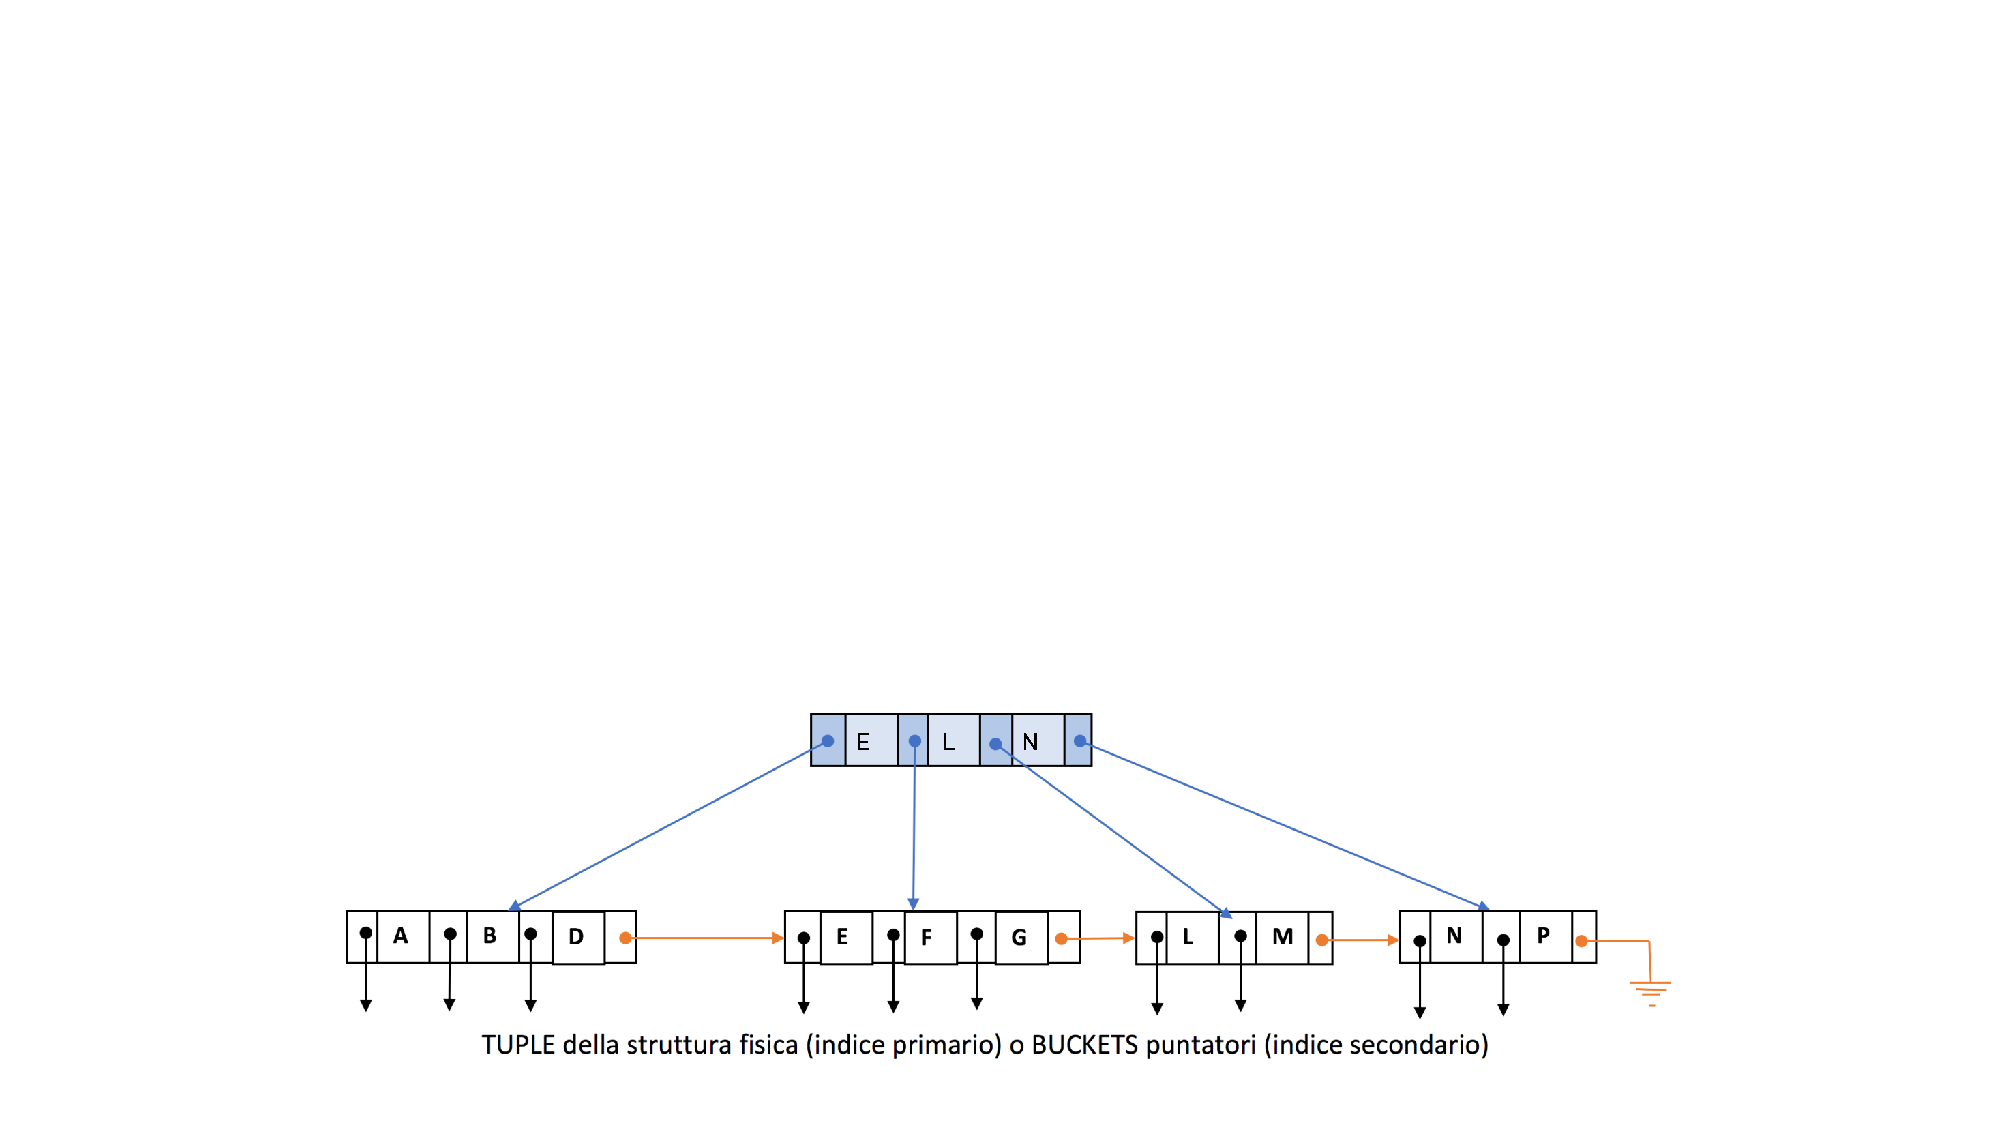
\includegraphics[width=\textwidth]{img/ex/b+-tree-1.pdf}
			\caption*{Esempio di albero B+-tree.}
		\end{figure}
		
		\noindent
		Operazione di \textbf{ricerca}:
		\begin{enumerate}
			\item Si \textbf{cerca} nel nodo radice il \textbf{più piccolo valore di chiave maggiore del valore di chiave di ricerca} K:
			\begin{itemize}
				\item Se esiste, allora si segue il puntatore relativo;
				
				\item Se non esiste, viene seguito l'ultimo puntatore presente nel nodo.
			\end{itemize}
			
			\item Una volta \textbf{raggiunto il nodo foglia}, viene \textbf{cercato} il valore K (\textbf{chiave di ricerca}) nel nodo:
			\begin{itemize}
				\item Se viene trovato il valore, si prosegue la strada verso le tuple;
				
				\item Se non esiste, si ritorna al passo 1.
			\end{itemize}
		\end{enumerate}\newpage
		
		\begin{table}[!htp]
			\centering
			\begin{tabular}{@{} l p{23em} @{}}
				\toprule
				Concetto & Definizione \\
				\midrule
				Struttura 	& Un albero B+-tree è una struttura ad albero composta da nodi e legami:
				\begin{itemize}
					\item \textbf{Nodi}, identificano le \textbf{pagine della memoria secondaria};
					
					\item \textbf{Legami}, collegano i nodi e rappresentano i \textbf{puntatori ad ogni pagina}.
				\end{itemize} \\ 
				%
				Op. ricerca	& L'operazione di ricerca si divide in \textbf{due fasi}:
				\begin{enumerate}
					\item \textbf{Cercare} nel nodo radice il \textbf{più piccolo valore di chiave maggiore del valore di chiave di ricerca}. Se trovato, si \textbf{segue} il relativo \textbf{puntatore}, altrimenti viene \textbf{seguito l'ultimo puntatore presente nel nodo};
					
					\item Raggiunto il \textbf{nodo foglia}, viene \textbf{cercato il valore della chiave di ricerca}. Se trovato, si segue la \textbf{strada verso la tupla}, altrimenti si \textbf{torna al punto 1}.
				\end{enumerate} \\
				\bottomrule
			\end{tabular}
			\caption{Riepilogo dei concetti della domanda sugli alberi B+-tree.}
		\end{table}\newpage
		
		\item \textbf{(\emph{2 punti})} \textcolor{Green4}{\textbf{\emph{Illustrare il meccanismo di 2PL stretto.}}}\label{dom: 2PL stretto}
		
		Il locking a due fasi stretto (2PL stretto) è un principio che afferma: \textbf{i lock di una transazione possono essere rilasciati solo dopo aver correttamente effettuato le operazioni di commit/abort}.
		
		La conseguenza di questo metodo è che i lock vengono rilasciati solo al termine della transazione, ovvero una volta raggiunto lo stato finale.
		
		Il \textbf{vantaggio principale} riguarda l'\textbf{impossibilità} di verificarsi del fenomeno di \textbf{letture sporche}. Questo \textbf{perché viene impedito l'accesso, da parte di altre transazioni, ai dati scritti da transazioni che ancora non hanno effettuato il \textsf{commit}}.
		
		\begin{table}[!htp]
			\centering
			\begin{tabular}{@{} l p{25em} @{}}
				\toprule
				Concetto & Descrizione \\
				\midrule
				Definizione & Il 2PL stretto afferma che i \textbf{lock di una transazione possono essere rilasciati solo dopo aver correttamente effettuato le operazioni di \textsf{commit}/\text{abort}}. \\ [.7em]
				%
				Conseguenza & I lock vengono rilasciati solo al termine della transazione, ovvero al raggiungimento dello stato finale. \\ [.7em]
				%
				Vantaggio	& Il fenomeno di \textbf{\dquotes{lettura sporca} non può verificarsi poiché viene impedito l'accesso, da parte di altre transazioni, ai dati scritti da transazioni che ancora non hanno effettuato il \textsf{commit}}. \\ 
				\bottomrule
			\end{tabular}
			\caption{Riepilogo dei concetti della domanda sul 2PL stretto.}
		\end{table}
	\end{enumerate}\newpage
	
	Domande di teoria tratte dalla terza prova intermedia dell'esame 10/06/2022.
	\begin{enumerate}
		\item \textbf{(\emph{2 punti})} \textcolor{Green4}{\textbf{\emph{Illustrare le proprietà delle transazioni ed indicare da quali moduli del DBMS vengono garantite.}}}
		
		Risposta a pagina \pageref{dom: proprietà delle transazioni}.		
		
		\item \textbf{(\emph{3 punti})} \textcolor{Green4}{\textbf{\emph{Si presenti la definizione di View-serializzabilità e la relazione tra l'insieme degli schedule VSR e l'insieme degli schedule CSR. Presentare la dimostrazione formale di tale relazione.}}}\label{dom: view-serializzabilità, relazione VSR e CSR + dimostrazione}
		
		Prima di dare la dimostrazione di view-serializzabile, è necessario dare tre definizioni:
		\begin{enumerate}
			\item Un'operazione di lettura $r_{i}\left(x\right)$ si definisce \dquotes{\textbf{legge da}} quando una scrittura $w_{j}\left(x\right)$ di un'altra transazione sulla stessa risorsa precede la lettura $r_{i}\left(x\right)$ sulla stessa risorsa. Inoltre, non ci deve essere alcuna scrittura $w_{k}\left(x\right)$ appartenente ad un'altra transazione tra le due operazioni ($r_{i}\left(x\right)$ e $w_{j}\left(x\right)$).
			
			\item Un'operazione di scrittura $w_{i}\left(x\right)$ viene definita \dquotes{\textbf{scrittura finale}} se è l'ultima scrittura dell'oggetto $x$ che appare nello schedule.
			
			\item \textbf{Due schedule} vengono definiti \textbf{view-equivalenti} se posseggono la \textbf{stessa relazione \dquotes{legge da} e le stesse \dquotes{scritture finali}}.
		\end{enumerate}
		\textbf{Uno schedule viene detto view-serializzabile se esiste uno schedule seriale view-equivalente ad esso}. L'insieme degli schedule seriali view-equivalenti ad esso si chiama VSR.
		
		Inoltre, esiste una \textbf{relazione tra l'insieme VSR e l'insieme dei conflict-serializzabili (CSR)}:
		\begin{equation*}
			CSR \subset VSR
		\end{equation*}
		Ovvero, se uno \textbf{schedule è CSR, allora è anche VSR allo stesso tempo, ma non viceversa!}\newpage
		
		\noindent
		\begin{proof}[\textbf{Dimostrazione} $CSR \Longrightarrow VSR$]
			Si supponga che lo schedule $S_{1}$ abbia uno schedule seriale conflict-equivalente a $S_{2}$. Allora si dimostra che lo schedule $S_{1}$ ha come schedule seriale view-equivalente $S_{2}$.\newline
			
			\noindent
			Dato che $S_{2}$ è uno schedule seriale conflict-equivalente a $S_{1}$, allora:
			\begin{itemize}
				\item L'insieme delle scritture finali di $S_{1}$ è uguale all'insieme delle scritture finali di $S_{2}$:
				\begin{equation*}
					\text{Scritture finali } S_{1} = \text{Scritture finali } S_{2}
				\end{equation*}
				Ipotizzando per assurdo il contrario, allora esisterebbero due scritture sulla stessa risorsa in ordine diverso. Tuttavia, dato che le due scritture sarebbero in conflitto, i due schedule non sarebbero conflict-equivalenti.
				
				\item L'insieme dei \dquotes{legge da} di $S_{1}$ è uguale all'insieme dei \dquotes{legge da} di $S_{2}$:
				\begin{equation*}
					\text{Legge da } S_{1} = \text{Legge da } S_{2}
				\end{equation*}
				Ipotizzando per assurdo il contrario, allora esisterebbero due scritture in ordine diverso o coppie lettura-scrittura in ordine diverso. Tuttavia, come sopra, dato che le due scritture sarebbero in conflitto, i due schedule non sarebbero conflict-equivalenti.
			\end{itemize}
		\end{proof}
		
		\begin{table}[!htp]
			\centering
			\begin{tabular}{@{} l p{21em} @{}}
				\toprule
				Concetto & Definizione \\
				\midrule
				Def. legge da 						& Quando, data una risorsa, una \textbf{scrittura di un'altra transizione precede una lettura di un'altra transazione sulla stessa risorsa}. Inoltre, \textbf{non ci deve essere una scrittura da parte di un'altra transizione}, su tale risorsa, tra le due operazioni citate. \\ [.7em]
				Def. scrittura finale 				& Quando è l'\textbf{ultima scrittura dell'oggetto $x$ che appare nello schedule}. \\ [.7em]
				Def. view-equivalenza				& Se \textbf{due schedule hanno la stessa relazione legge da e le stesse scritture finali}. \\ [.7em]
				Dimostrazione $CSR \Rightarrow VSR$	& Vedere sopra. \\
				\bottomrule
			\end{tabular}
			\caption{Riepilogo dei concetti della domanda sulla view-serializzabilità e la relazione tra VSR e CSR.}
		\end{table}\newpage
		
		\item \textbf{(\emph{2 punti})} \textcolor{Green4}{\textbf{\emph{Lo studente illustri la struttura di accesso ai dati denominata indice secondario, si descrivano in particolare i seguenti punti: (i) le caratteristiche della struttura di accesso, (ii) l'algoritmo di ricerca di una tupla con chiave K usando l'indice.}}}\label{dom: indice secondario}
		
		L'\textbf{indice secondari}o utilizza una \textbf{chiave di ricerca} che \textbf{\underline{non} coincide con la chiave di ordinamento del file sequenziale}.
		
		\textbf{Ogni record} possiede:
		\begin{itemize}
			\item Un \textbf{valore} della \textbf{chiave di ricerca}
			
			\item \textbf{Puntatore al bucket di puntatori che individuano nel file sequenziale tutte le tuple con valore di chiave uguale al valore della chiave di ricerca}
		\end{itemize}
		Inoltre, gli indici secondari \textbf{sono sempre densi}.
		
		\begin{figure}[!htp]
			\centering
			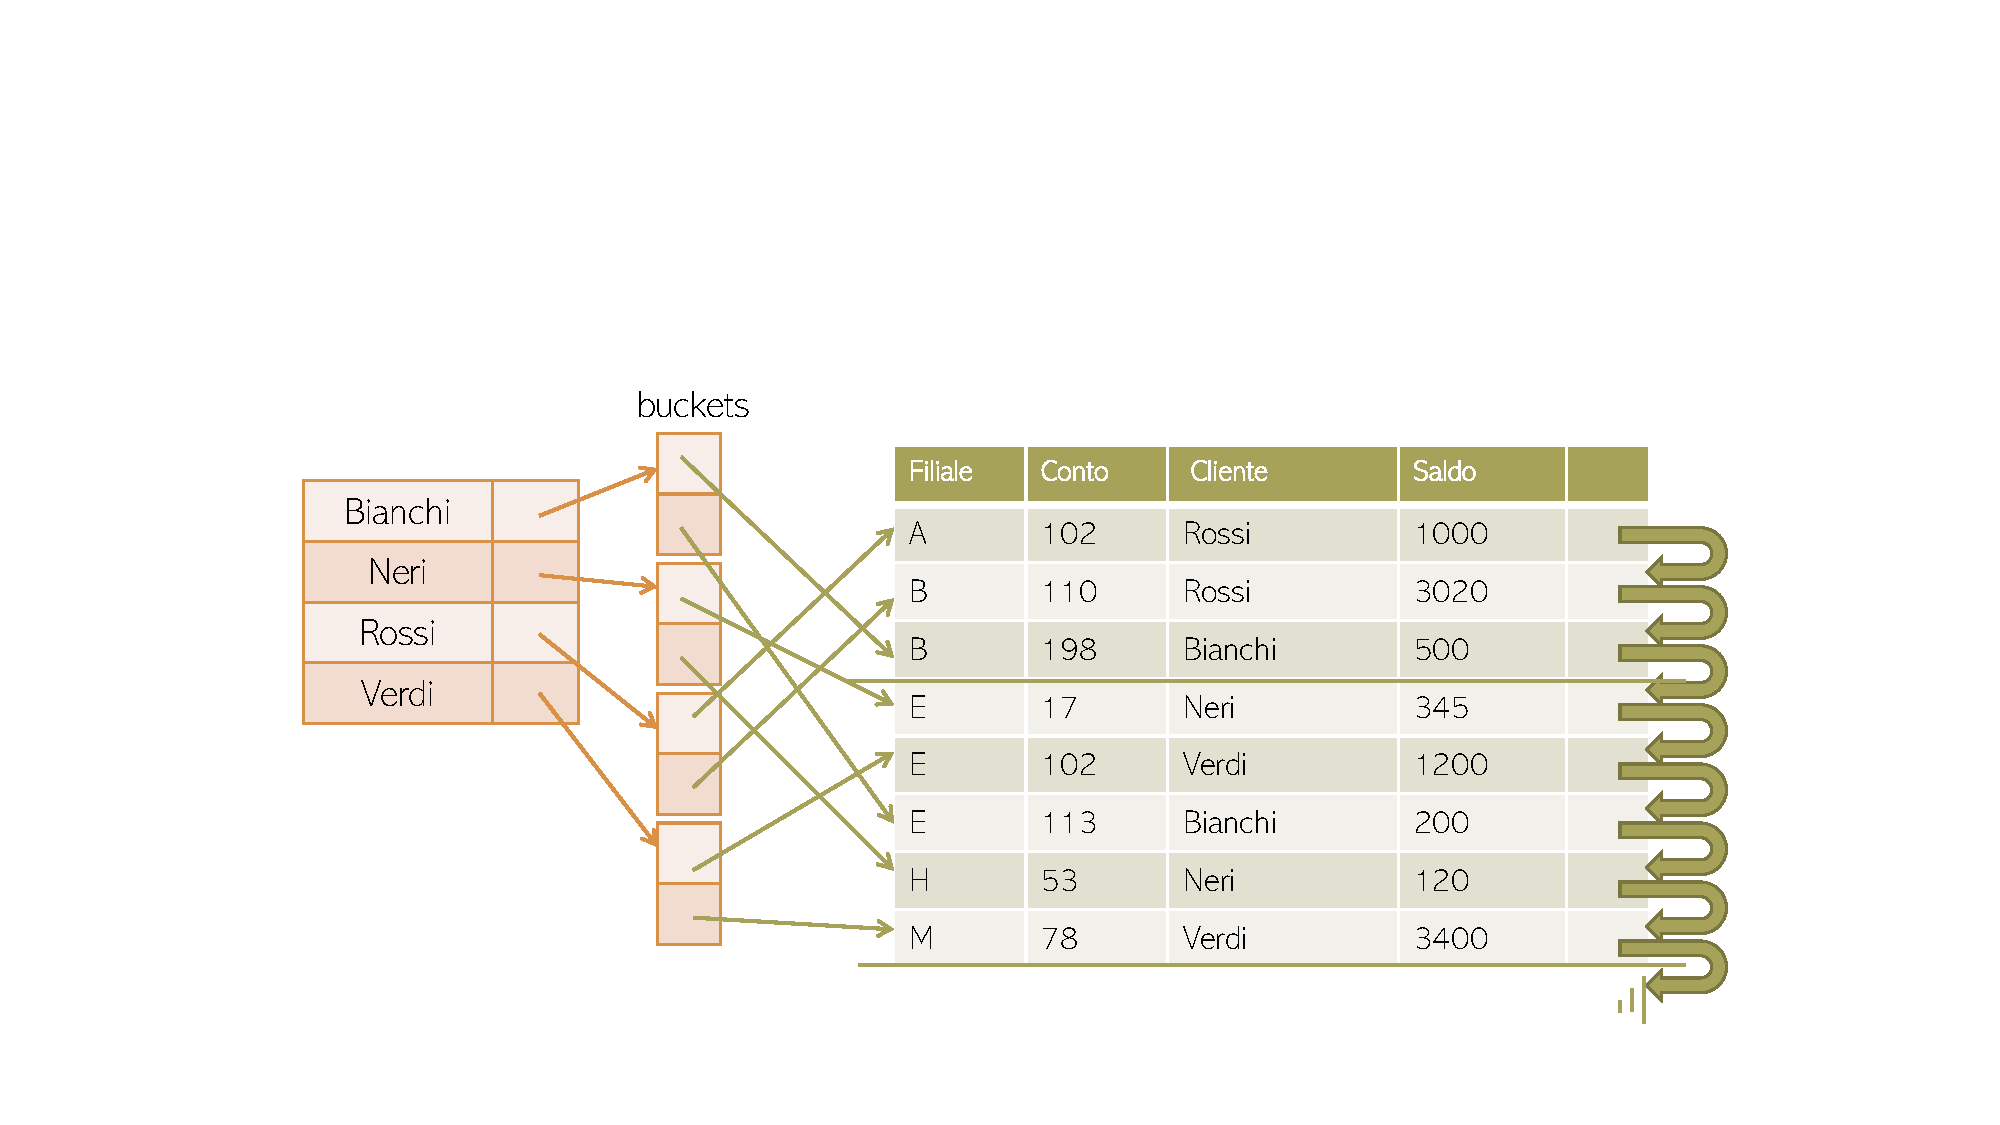
\includegraphics[width=\textwidth]{img/ex/indice-secondario-1.pdf}
		\end{figure}
		
		\noindent
		Operazione di \textbf{ricerca}:
		\begin{enumerate}
			\item \textbf{Scansione sequenziale dell'indice} per trovare il record
			
			\item \textbf{Accesso al bucket di puntatori} attraverso il puntatore presente dentro il record trovato
			
			\item \textbf{Accesso al file attraverso i puntatori del bucket} al quale è stato fatto l'accesso al punto precedente.
		\end{enumerate}
		\begin{equation*}
			\text{Costo} = 1 \text{ accesso indice } + 1 \text{ accesso al bucket } + n \text{ accessi pagine dati}
		\end{equation*}\newpage
		
		\begin{figure}[!htp]
			\centering
			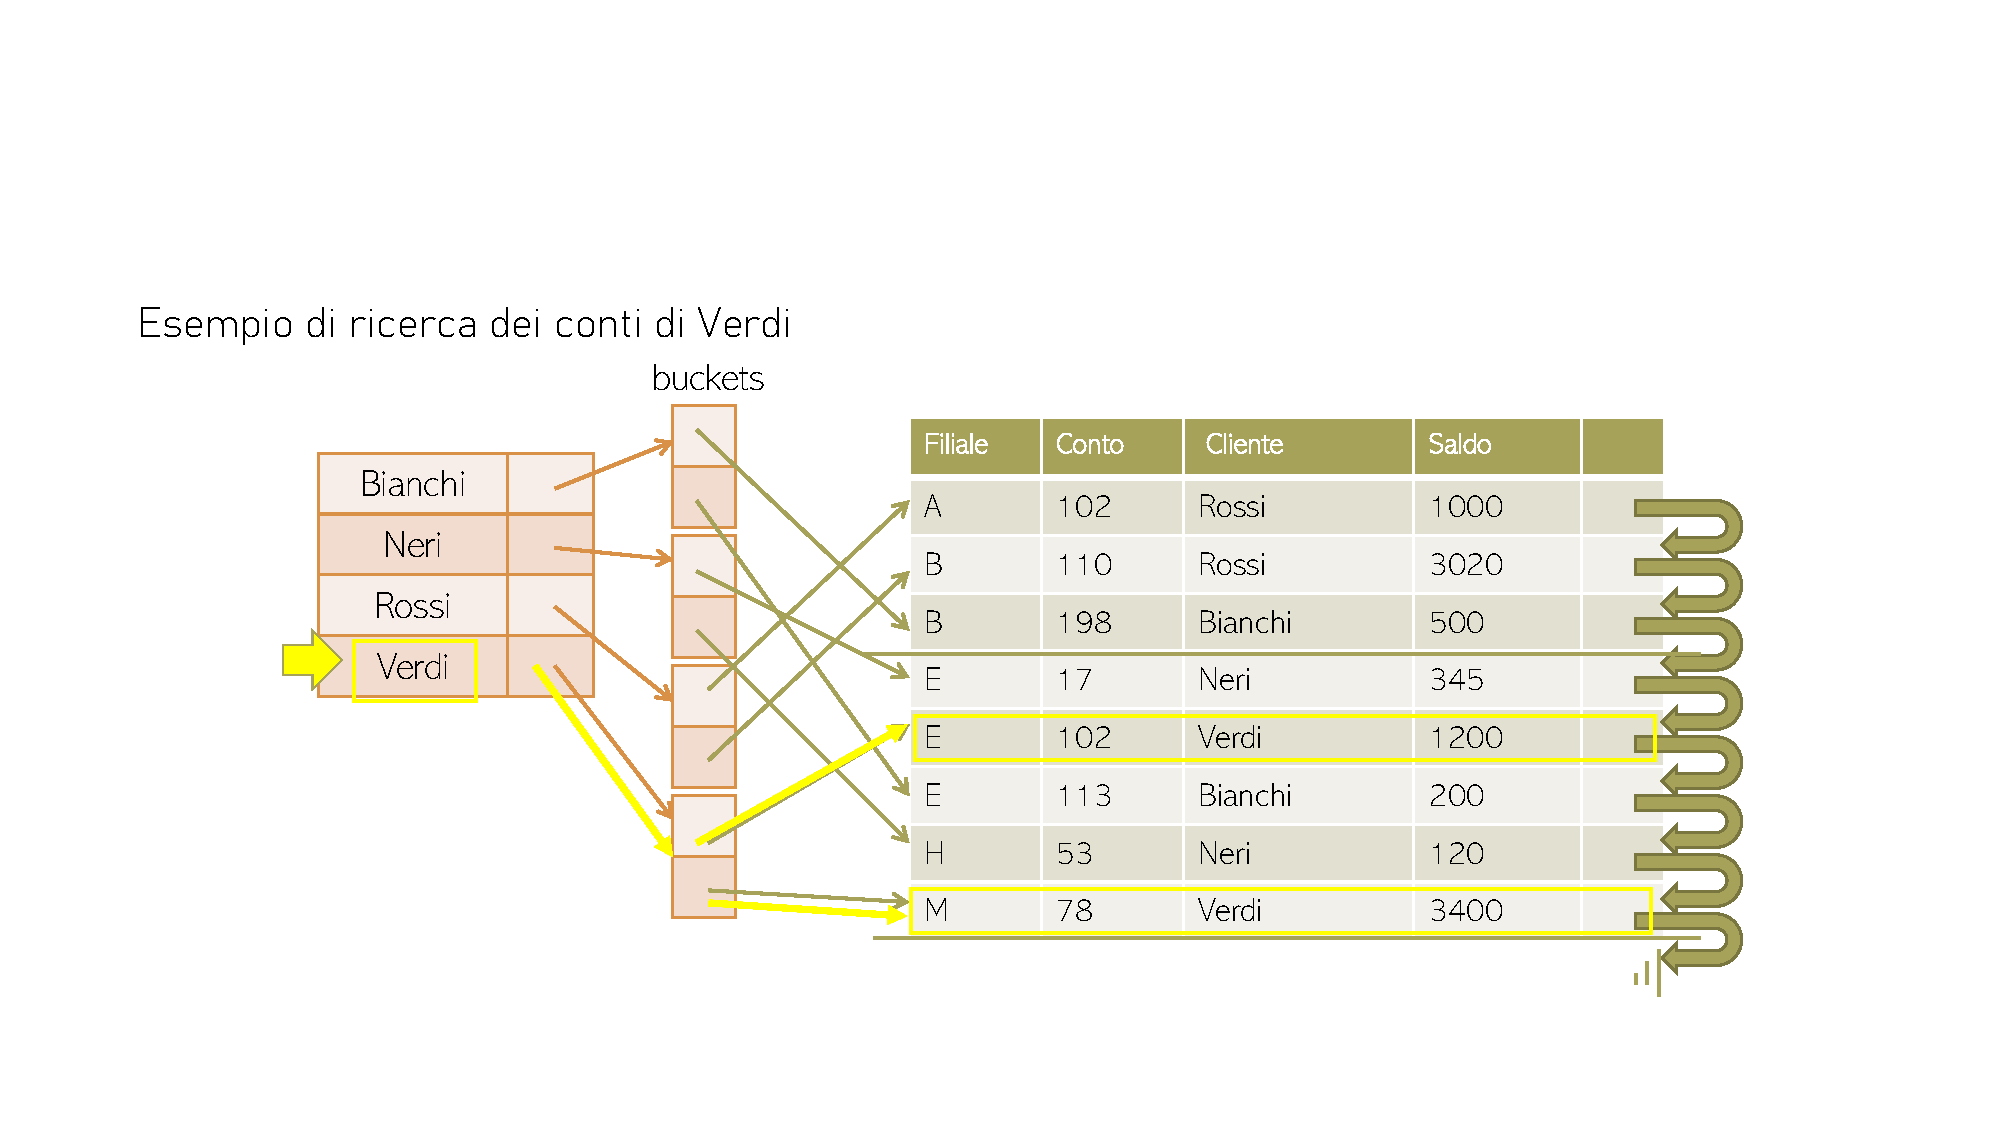
\includegraphics[width=\textwidth]{img/ex/indice-secondario-2.pdf}
		\end{figure}
		
		\begin{table}[!htp]
			\centering
			\begin{tabular}{@{} l p{23em} @{}}
				\toprule
				Concetto & Descrizione \\
				\midrule
				Definizione & Indice secondario usa una \textbf{chiave di ricerca che non coincide con la chiave di ordinamento del file sequenziale}. \\ [.7em]
				%
				Valori nel record & Ogni record ha due valori:
				\begin{enumerate}
					\item \textbf{Valore chiave di ricerca}
					
					\item \textbf{Puntatore al bucket di puntatori}, i quali individuano nel file sequenziale tutte le tuple con valore di chiave uguale al valore della chiave di ricerca.
				\end{enumerate} \\ [.7em]
				%
				Op. ricerca & La ricerca si divide in tre passi:
				\begin{enumerate}
					\item \textbf{Scansione sequenziale dell'indice} finché non viene trovato il record
					
					\item \textbf{Accesso al bucket dei puntatori} grazie al puntatore trovato nel record
					
					\item \textbf{Accesso al file sequenziale} grazie ai puntatori del bucket
				\end{enumerate}\\
				\bottomrule
			\end{tabular}
		\end{table}
		
		\item \textbf{(\emph{2 punti})} \textcolor{Green4}{\textbf{\emph{Lo studente illustri l'algoritmo di \underline{ripresa a caldo}.}}}
		
		Risposta a pagina \pageref{dom: ripresa a caldo}.
	\end{enumerate}\newpage
	
	% \section{Esami terzo parziale}
	
	% \subsection{Terzo parziale - 06/2015}
	
	% \subsection{Terzo parziale - 07/06/2016}
	
	% \subsection{Terzo parziale - 21/04/2022}
	
	% \subsection{Terzo parziale - 22/04/2022}
	
	% \subsection{Terzo parziale - 10/06/2022}\newpage
	
	\section{Indice delle domande}
	
	\subsection{Terzo parziale}
	
	\subsubsection{Domande teoriche}
	
	\begin{itemize}
		\item Illustrare l'architettura di un DBMS descrivendo in particolare il modulo di \textbf{gestione dei buffer}; si indichi inoltre, per ogni modulo dell'architettura, quali sono le proprietà delle transazioni che contribuisce a garantire.
		
		\emph{Risposta:} pagina \pageref{dom: gestione del buffer}
		
		\item Illustrare l'architettura di un DBMS descrivendo in particolare il modulo di \textbf{gestione dei guasti} (o gestore dell'affidabilità); si indichi inoltre, per ogni modulo dell'architettura, quali sono le proprietà delle transazioni che contribuisce a garantire.
		
		\emph{Risposta:} pagina \pageref{dom: gestione dei guasti}
		
		\item Illustrare le \textbf{proprietà delle transazioni}; si indichi inoltre quali moduli di un DBMS garantiscono ciascuna di tali proprietà.
		
		\emph{Risposta:} pagina \pageref{dom: proprietà delle transazioni}
		
		\item Illustrare il meccanismo di \textbf{2PL stretto}.
		
		\emph{Risposta:} pagina \pageref{dom: 2PL stretto}
		
		%%%%%%%%%%%%%%%%%%%%%%%%%%%%%%%%%%%%%%%%%%%%%%%%%%%%%%%%%%%%%%%%%%
		\longline
		%%%%%%%%%%%%%%%%%%%%%%%%%%%%%%%%%%%%%%%%%%%%%%%%%%%%%%%%%%%%%%%%%%
		
		\item Si presenti in dettaglio la definizione di \textbf{Conflict-Serializzabilità (CSR)}.
		
		\emph{Risposta:} pagina \pageref{dom: CSR - Conflict-Serializzabilità}
		
		\item Si presenti in dettaglio la \textbf{politica di concessione dei lock} applicata dal gestore dell'esecuzione concorrente secondo la tecnica detta \dquotes{Locking a due fasi}.
		
		\emph{Risposta:} pagina \pageref{dom: politica di concessione dei lock - locking a due fasi}
		
		\item Si presenti in dettaglio la \textbf{definizione di conflict-equivalenza} tra due schedule.
		
		\emph{Risposta:} pagina \pageref{dom: conflict-equivalenza}
		
		\item Si presenti in dettaglio la \textbf{definizione di view-equivalenza} tra due schedule.
		
		\emph{Risposta:} pagina \pageref{dom: view-equivalenza}
		
		\item Si presenti la definizione di \textbf{View-Serializzabilità (VSR)} e la \textbf{relazione} tra l'insieme degli schedule \textbf{VSR} e l'insieme degli schedule \textbf{CSR}. Presentare la dimostrazione formale di tale relazione.
		
		\emph{Risposta:} pagina \pageref{dom: view-serializzabilità, relazione VSR e CSR + dimostrazione}
		
		%%%%%%%%%%%%%%%%%%%%%%%%%%%%%%%%%%%%%%%%%%%%%%%%%%%%%%%%%%%%%%%%%%
		\longline
		%%%%%%%%%%%%%%%%%%%%%%%%%%%%%%%%%%%%%%%%%%%%%%%%%%%%%%%%%%%%%%%%%%
		
		\item Lo studente illustri la struttura di accesso ai dati denominata \textbf{indice primario denso}: caratteristiche della struttura, ricerca, inserimento e cancellazione di entry dall'indice.
		
		\emph{Risposta:} pagina \pageref{dom: indice primario denso}
		
		\item Lo studente illustri la struttura di accesso ai dati denominata \textbf{indice primario sparso}, si descrivano in particolare i seguenti punti: (i) le caratteristiche della struttura di accesso, (ii) l'algoritmo di ricerca di una tupla con chiave K usando l'indice.
		
		\emph{Risposta:} pagina \pageref{dom: indice primario sparso}
		
		\item Lo studente illustri la struttura di accesso ai dati denominata \textbf{struttura ad accesso calcolato (hashing)}, si descrivano in particolare i seguenti punti: (i) le caratteristiche della struttura di accesso, (ii) l'algoritmo di ricerca di una tupla con chiave K usando l'indice.
		
		\emph{Risposta:} pagina \pageref{dom: struttura ad accesso calcolato - hashing}
		
		\item Lo studente illustri la struttura di accesso ai dati denominata \textbf{B+-tree}, si descrivano in particolare i seguenti punti: (i) le caratteristiche della struttura di accesso, (ii) l'algoritmo di ricerca di una tupla con chiave K usando l'indice.
		
		\emph{Risposta:} pagina \pageref{dom: B+-tree}
		
		\item Lo studente illustri la struttura di accesso ai dati denominata \textbf{indice secondario}, si descrivano in particolare i seguenti punti: (i) le caratteristiche della struttura di accesso, (ii) l'algoritmo di ricerca di una tupla con chiave K usando l'indice.
		
		\emph{Risposta:} pagina \pageref{dom: indice secondario}
		
		\item Lo studente illustri le differenze tra i costrutti \textbf{elemento} e \textbf{attributo} del linguaggio XML, mostrando un esempio di documento XML dove vengono utilizzati entrambi.
		
		\emph{Risposta:} pagina \pageref{dom: elemento e attributo in XML}
		
		\item Lo studente illustri l'algoritmo di \textbf{ripresa a caldo}.
		
		\emph{Risposta:} pagina \pageref{dom: ripresa a caldo}
	\end{itemize}\newpage
	
	\section{Terzo parziale - Temi d'esame}
	
	\subsection{Esame del 07/06/2016}
	
	\subsubsection{Domande di teoria}
	
	Le domande di teoria sono disponibili da pagina \pageref{dom: gestione dei guasti}.
	
	\longline
	
	\subsubsection{Esercizio 1 - Esecuzione concorrente}
	
	Dato il seguente schedule S:
	\begin{itemize}
		\item (2) indicare se è conflict-SR oppure no (calcolare l'insieme dei conflitti),
		
		\item (4) se non è CSR verificare se è view-SR oppure non-SR (giustificare dettagliatamente la risposta).
		\begin{equation*}
			S: r_{4}\left(t\right), \: w_{2}\left(t\right), \: r_{1}\left(t\right), \: r_{4}\left(y\right), \: r_{3}\left(y\right), \: w_{4}\left(y\right), \: w_{4}\left(z\right), \: w_{3}\left(z\right), \: w_{1}\left(t\right), \: w_{2}\left(x\right), \: w_{1}\left(z\right)
		\end{equation*}
	\end{itemize}
	
	\noindent
	\textcolor{Green4}{\textbf{\emph{\underline{Soluzione}}}}\newline
	
	\noindent
	Verifico se è CSR.\newline

	\noindent
	Le transazioni sono:
	\begin{equation*}
		\begin{array}{lll}
			T_{1} &:& r_{1}\left(t\right), \: w_{1}\left(t\right), \: w_{1}\left(z\right) \\
			T_{2} &:& w_{2}\left(t\right), \: w_{2}\left(x\right) \\
			T_{3} &:& r_{3}\left(y\right), \: w_{3}\left(z\right) \\
			T_{4} &:& r_{4}\left(t\right), \: r_{4}\left(y\right), \: w_{4}\left(y\right), \: w_{4}\left(z\right) 
		\end{array}
	\end{equation*}
	Calcolo l'insieme dei conflitti:
	\begin{itemize}
		\item $\textcolor{Red3}{r_{4}\left(t\right)}, \: \textcolor{Red3}{w_{2}\left(t\right)}, \: r_{1}\left(t\right), \: r_{4}\left(y\right), \: r_{3}\left(y\right), \: w_{4}\left(y\right), \: w_{4}\left(z\right), \: w_{3}\left(z\right), \: w_{1}\left(t\right), \: w_{2}\left(x\right), \: w_{1}\left(z\right)$
		
		\item $\textcolor{Red3}{r_{4}\left(t\right)}, \: w_{2}\left(t\right), \: r_{1}\left(t\right), \: r_{4}\left(y\right), \: r_{3}\left(y\right), \: w_{4}\left(y\right), \: w_{4}\left(z\right), \: w_{3}\left(z\right), \: \textcolor{Red3}{w_{1}\left(t\right)}, \: w_{2}\left(x\right), \: w_{1}\left(z\right)$
		
		\item $r_{4}\left(t\right), \: \textcolor{Red3}{w_{2}\left(t\right)}, \: \textcolor{Red3}{r_{1}\left(t\right)}, \: r_{4}\left(y\right), \: r_{3}\left(y\right), \: w_{4}\left(y\right), \: w_{4}\left(z\right), \: w_{3}\left(z\right), \: w_{1}\left(t\right), \: w_{2}\left(x\right), \: w_{1}\left(z\right)$
		
		\item $r_{4}\left(t\right), \: \textcolor{Red3}{w_{2}\left(t\right)}, \: r_{1}\left(t\right), \: r_{4}\left(y\right), \: r_{3}\left(y\right), \: w_{4}\left(y\right), \: w_{4}\left(z\right), \: w_{3}\left(z\right), \: \textcolor{Red3}{w_{1}\left(t\right)}, \: w_{2}\left(x\right), \: w_{1}\left(z\right)$
		
		\item $r_{4}\left(t\right), \: w_{2}\left(t\right), \: r_{1}\left(t\right), \: r_{4}\left(y\right), \: \textcolor{Red3}{r_{3}\left(y\right)}, \: \textcolor{Red3}{w_{4}\left(y\right)}, \: w_{4}\left(z\right), \: w_{3}\left(z\right), \: w_{1}\left(t\right), \: w_{2}\left(x\right), \: w_{1}\left(z\right)$
		
		\item $r_{4}\left(t\right), \: w_{2}\left(t\right), \: r_{1}\left(t\right), \: r_{4}\left(y\right), \: r_{3}\left(y\right), \: w_{4}\left(y\right), \: \textcolor{Red3}{w_{4}\left(z\right)}, \: \textcolor{Red3}{w_{3}\left(z\right)}, \: w_{1}\left(t\right), \: w_{2}\left(x\right), \: w_{1}\left(z\right)$
		
		\item $r_{4}\left(t\right), \: w_{2}\left(t\right), \: r_{1}\left(t\right), \: r_{4}\left(y\right), \: r_{3}\left(y\right), \: w_{4}\left(y\right), \: \textcolor{Red3}{w_{4}\left(z\right)}, \: w_{3}\left(z\right), \: w_{1}\left(t\right), \: w_{2}\left(x\right), \: \textcolor{Red3}{w_{1}\left(z\right)}$
		
		\item $r_{4}\left(t\right), \: w_{2}\left(t\right), \: r_{1}\left(t\right), \: r_{4}\left(y\right), \: r_{3}\left(y\right), \: w_{4}\left(y\right), \: w_{4}\left(z\right), \: \textcolor{Red3}{w_{3}\left(z\right)}, \: w_{1}\left(t\right), \: w_{2}\left(x\right), \: \textcolor{Red3}{w_{1}\left(z\right)}$
	\end{itemize}
	Quindi l'insieme dei conflitti è:
	\begin{equation*}
		\begin{array}{lll}
			\text{Conflitti}\left(S\right) = \{ & \left(r_{4}\left(t\right) \: w_{2}\left(t\right)\right), \left(r_{4}\left(t\right) \: w_{1}\left(t\right)\right), & \\
												& \left(w_{2}\left(t\right) \: r_{1}\left(t\right)\right), \left(w_{2}\left(t\right) \: w_{1}\left(t\right)\right), & \\
												& \left(r_{3}\left(y\right) \: w_{4}\left(y\right)\right),  														& \\
												& \left(w_{4}\left(z\right) \: w_{3}\left(z\right)\right), \left(w_{4}\left(z\right) \: w_{1}\left(z\right)\right), & \\
												& \left(w_{3}\left(z\right) \: w_{1}\left(z\right)\right) &	\}
		\end{array}
	\end{equation*}\newpage

	\noindent
	Adesso si costruisce il grafo:
	\begin{figure}[!htp]
		\centering
		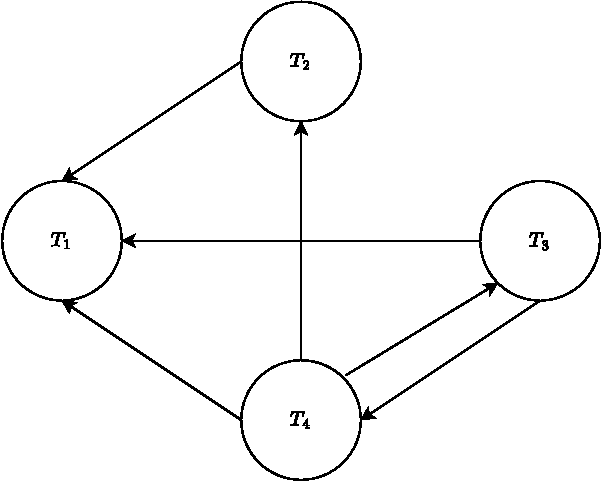
\includegraphics[width=.7\textwidth]{img/CSR-4.pdf}
	\end{figure}

	\noindent
	Il grafo non è aciclico, quindi non è CSR. Si verifica se è VSR.\newline

	\noindent
	Si costruisce l'insieme LeggeDa e ScrittureFinali:
	\begin{equation*}
		\begin{array}{lll}
			\text{LeggeDa}\left(S\right) 			&=& \left\{\left(r_{1}\left(t\right) \: w_{2}\left(t\right)\right)\right\} \\
			\text{ScrittureFinali}\left(S\right)	&=& \left\{w_{4}\left(y\right), w_{1}\left(t\right), w_{2}\left(x\right), w_{1}\left(z\right)\right\}
		\end{array}
	\end{equation*}
	Si cerca una combinazione tale per cui sia VSR. Dal grafo si deduce che $T_{1}$ deve essere l'ultimo valore poiché non ha grafi orientati in uscita:
	\begin{equation*}
		\cdots T_{1}
	\end{equation*}
	La transazione $T_{2}$ ha l'unico grafo in entrata proveniente da $T_{4}$ e l'unico in uscita verso $T_{1}$, quindi:
	\begin{equation*}
		T_{3} \: T_{4} \: T_{2} \: T_{1}
	\end{equation*}
	Quindi $S$ è VSR.\newpage

	\subsubsection{Esercizio 2 - Ottimizzazione}

	Si consideri il seguente schema relazionale contenente le visite svolte in un ospedale:
	\begin{equation*}
		\begin{array}{ll}
			\textsf{PAZIENTE} & \left(\underline{CodiceSSN}, \text{Nome, Cognome, Ntelefono, Indirizzo, Città}\right) \\
			\textsf{VISITA} & \left(\underline{CodiceSSN, CFMedico, Data, OraInizio,} \text{Durata, PressioneArteriosaMin, PressioneArteriosaMax}\right) \\
			\textsf{MEDICO} & \left(\underline{CFMedico}, \text{Cognome, Nome, Specialita}\right)
		\end{array}
	\end{equation*}
	
	\subsubsection{Esercizio 3 - B+-tree}
	
	\subsubsection{Esercizio 4 - XML}
\end{document}